\documentclass[hidelinks,12pt,a4paper,twoside]{article}

\usepackage[utf8]{inputenc}
% Paket für die Anpassung von Layout und Abständen
\usepackage{setspace} 	
\usepackage{array} 
\usepackage{tocloft}

\usepackage[bottom,hang,stable]{footmisc}
\usepackage[font=small]{caption}
\usepackage{subcaption}


\setlength{\cftsubsecnumwidth}{3em}

\makeatletter                               
\renewcommand*\l@table{\@dottedtocline{1}{3em}{5em}}
\renewcommand*\l@figure{\@dottedtocline{1}{1.5em}{4em}}
\makeatother

\usepackage{longtable}

\usepackage{graphicx} % Required for inserting images
\usepackage{fancyhdr}

\usepackage{amssymb}
% Überschriftenabstand anpassen
\usepackage{titlesec}
\usepackage[ngerman]{babel}
\usepackage[document]{ragged2e}
\usepackage[top=3.5cm,left=3cm,right=2cm,bottom=2.5cm,headsep=0.3in,headheight=1in]{geometry}

\usepackage{charter}
\usepackage{adjustbox}
\usepackage{csquotes}
\usepackage[citestyle=authortitle, backend=bibtex]{biblatex}
\usepackage{minted}
\usepackage{picinpar}
\usepackage{wrapfig}
\usepackage{pdfpages} %pdf 
\usepackage{varwidth}
\usepackage{hyperref} % Paket für Hyperlinks
					
					
				
\usepackage{amsmath} 	

\usepackage{listings,xcolor}
\usepackage{listingsutf8} 
\usepackage{float} 
\usepackage{footnote}
\usepackage{enumitem}
\usepackage{longtable}

\usepackage{bold-extra}


% allgemein gültige Formateinstellungen
% -------------------------------------
\renewcommand{\familydefault}{\sfdefault} 	% set Font-Family to a similar font like Arial
\raggedbottom 								% Abschnitte werden nicht auseinander gezogen, um den restlichen Platz auf einer Seite zu füllen
%\raggedright 								% gesamtes Dokument linksbündig (auch Paragraphen) OHNE Silbentrennung

\usepackage{ragged2e}						% gesamtes Dokument linksbündig (auch Paragraphen) MIT Silbentrennung
\RaggedRight

\onehalfspacing 							% 1.5-facher Abstand zwischen den Zeilen

\renewcommand{\arraystretch}{1.05} 			% Vergrößerung des Abstands zwischen den Tabellenzeilen
\newcolumntype{C}[1]{>{\centering\arraybackslash}p{#1}} % erstellen eines Spaltentyps mit zentriertem Inhalt unter der Angabe einer Spaltenbreite
\newcolumntype{L}[1]{>{\raggedright\arraybackslash}p{#1}} % erstellen eines Spaltentyps mit linksbündigem Inhalt unter der Angabe einer Spaltenbreite

\setlength{\footnotemargin}{0.5cm} 			% Abstand zwischen Fußnotennummer und -text
\setlist{nosep} 							% zusätzliche Abstände bei Aufzählungen entfernen
\setlength{\parskip}{1em} 					% Abstand nach einem Absatz

\skip\footins 30pt

% Abstände vor und nach Überschriften auf den verschiedenen Ebenen
\titlespacing\section       {0pt}{0pt plus 0pt minus 1pt}{0pt plus 1pt minus 1pt}
\titlespacing\subsection    {0pt}{0pt plus 0pt minus 1pt}{0pt plus 1pt minus 1pt}
\titlespacing\subsubsection {0pt}{0pt plus 0pt minus 1pt}{0pt plus 1pt minus 1pt}


\newcommand{\nameSH}{Sophia Hagen }
\newcommand{\nameJS}{Julius Scherrer }
\newcommand{\nameSB}{Sebastian Bellai }
\newcommand{\nameCZ}{Constantin Zumtobel }
\newcommand{\supverisor}{Dipl.-Ing. Bischof Gerold}
\newcommand{\klasse}{5AHEL und 5BHEL}
\newcommand{\Thema}{Test Station for CubeSat STS1}
\newcommand{\pjname}{Test Station for CubeSat STS1}
\newcommand{\DADate}{05.04.2024}
\newcommand{\school}{HTL Rankweil}
\newcommand{\raspi}{Raspberry Pi }
\newcommand{\HRule}[1]{\rule{\linewidth}{#1}}
\newcommand*{\quelle}{%
  \autocite{Quelle:}
}
\newcommand{\PrintDate}{05.04.2024} 

\addbibresource{sophisnachschlagwerk}

\fancyhf{} % Löscht alle voreingestellten Kopf- und Fußzeilen

\lhead{\hspace{0.2cm} 
\includegraphics[height=1.04cm]{image/htlr_logo.png}}
\chead{\textbf{HTBLuVA  Rankweil} 
	\\[0.05in]
	\footnotesize{\textit{Höhere Lehranstalt für Elektronik und Technische Informatik}}}
\rhead{
\includegraphics[height=1.04cm]{image/htl_logo.jpg} \hspace{0.2cm}}
\newcommand\SecAuth[1]{\def\@SecAuth{#1}}
\pagestyle{fancy}
%\fancyfoot{}

\begin{document}

%
\title{\textsc{Diplomarbeit}
		\\ 
		
		\textbf{\uppercase{Test Station for CubeSat STS1}}
		\HRule{2pt} \\ 
		\textsc{Abschlussjahrgang 2023/2024}  \vspace*{5\baselineskip}}

\date{}

\author{
		\school\\
        \klasse\\
         \nameSH, \nameJS, \nameCZ, \nameSB\\ 
		}

 schöne Titelseite
%\maketitle schöne Titelseite
%\thispagestyle{empty} schöne titelseite
\begin{center}
	\textbf {\huge {\uppercase {Diplomarbeit}}}
	\par \textbf {\huge {\uppercase {\Thema}}}
	\vspace{0.3cm}
	
    \vspace{10mm}
	
\includegraphics[scale=1.5]{image/logodiplo.png}
\end{center}

\vfill % damit der folgende am Blattende positioniert wird


    \begin{tabular}{lcl}
        \vspace{3mm}
       \textbf{Ausgeführt im Schuljahr 2023/2024 von:}  &  & \textbf{Betreuer}\\
       \vspace{3mm}
        \nameSH & 5BHEL & \supverisor \\ 
        \vspace{3mm}
        \nameJS & 5BHEL &\\
        \vspace{3mm}
        \nameCZ & 5BHEL & \\
        \vspace{3mm}
        \nameSB & 5AHEL& \\
    \end{tabular}
    


\par Rankweil, am \PrintDate \\		

\noindent\rule{\textwidth}{0.4pt}
Abgabevermerk:
\linebreak

\begin{tabular}{p{7cm}C{6cm}}
	\hspace{1cm} DA original, am \PrintDate & ........................................ \\ 
	& Dipl.-Ing. Bischof Gerold \\ [2.5em]
	
	\hspace{1cm} DA digital, am \PrintDate & ........................................ \\ 
	& Dipl.-Ing. Bischof Gerold \\
\end{tabular}
\newpage
\input{eidestattlicherklärung}
\newpage
\tableofcontents
\newpage

\fancyfoot[LE,RO]{\thepage}
	\fancyfoot[LO,RE]{\DADate~\textbar~\pjname~\textbar ~\@SecAuth}
	\renewcommand{\footrulewidth}{0.4pt} % anzeigen Separator-Strich in der Fußzeile 
	\onehalfspacing
\renewcommand{\thepage}{\arabic{page}} % ab hier arabische Fußzeile
\SecAuth{\nameSH}


\section{Diplomarbeit Dokumentation}
\vspace{3mm}
 Verfasser/in:\\
\nameSH, \nameJS, \nameCZ, \nameSB\\ 
\vspace{3mm}
Klassen/Schuljahr: \klasse, Schuljahr 2023/2024\\
\vspace{3mm}
Thema der Diplomarbeit: \Thema\\
\vspace{3mm}
Kooperationspartner: TU Wien Space Team\autocite{TU_Wien_Spaceteam}, Omicron electronics GmbH\autocite{OMICRON_electronics_GmbH}, Bachmann electronic GmbH\autocite{Bachmann_electronic_GmbH}, Hefel Technik GmbH\autocite{Hefel_Technik_GmbH}, Tschabrun Hermann Gesellschaft m.b.H.\autocite{Tschabrun_Hermann_Gesellschaft}, Robotunits GmbH\autocite{robogmbh}, Spectra-Physics \autocite{Spectra} \\
\vspace{3mm}
Aufgabenstellung:\\
Es soll eine Teststation entwickelt werden,die die Zuverlässigkeit des CubeSats testet. Der CubeSat ist ein kleiner Satelitt der vom SpaceTeam der TU-Wien entwickelt wurde.\\    

%\newpage

\section{Zusammenfassung}
{Das Spaceteam der TU-Wien benötigt eine Teststation, um die Zuverlässigkeit des CubeSat zu überprüfen. Dafür soll eine Kammer gebaut werden, in der verschiedene Tests mit dem Satelliten durchgeführt werden können. Die Kammer soll bei einer Temperatur von 0°C bis 30°C betrieben werden können. In der Kammer befinden sich verschiedene Sensoren, um einen Vergleich zwischen den Sensoren auf dem CubeSat und in der Teststation herzustellen. Durch diesen Ist-Soll Vergleich können Fehler auf dem CubeSat erkannt werden und fehlerhafte Bauteile ausgetauscht werden. Um diesen Ist-Soll-Vergleich zu veranschaulichen und um alle Komponenten anzusteuern, soll eine benutzerfreundliche Webapplikation entwickelt werden. Mithilfe eines Gyroskops wird der CubeSat in x-, y- und z-Richtung rotiert. Mit den Sensoren auf dem Satelitt können die Auswirkungen dieser Rotation erfasst werden und mithilfe der Webapplikation dargestellt werden.}
\newpage

{\raggedright
\section{Diploma Thesis Documentation}
\vspace{3mm}
 Author(s):\\
 \nameSH, \nameJS, \nameCZ, \nameSB\\ 
\vspace{3mm}
 Class/ Academic year: 5BHEL and 5AHEL, 2023/2024
\vspace{3mm}
 Diplo Thesis Topic: \Thema\\
\vspace{3mm}
 Cooperation Partners: TU Wien Space Team\autocite{TU_Wien_Spaceteam}, Omicron electronics GmbH\autocite{OMICRON_electronics_GmbH}, Bachmann electronic GmbH\autocite{Bachmann_electronic_GmbH}, Hefel Technik GmbH\autocite{Hefel_Technik_GmbH}, Tschabrun Hermann Gesellschaft m.b.H.\autocite{Tschabrun_Hermann_Gesellschaft}, Robotunits GmbH\autocite{robogmbh}\\
\vspace{3mm}
 Assignment of Tasks:\\
 A test station is to be developed that tests the reliability of the CubeSat. The CubeSat is a small satellite developed by the SpaceTeam at TU Vienna.\\    
}
%\newpage
\section{Abstract}
The TU Vienna space team needs a test station to check the reliability of the CubeSat. For this purpose, a chamber is to be built in which various tests can be carried out with the satellite. The chamber should be able to operate at a temperature of 0°C to 30°C. There are various sensors in the chamber to make a comparison between the sensors on the CubeSat and in the test station. Through this actual-target comparison, errors on the CubeSat can be identified and faulty components can be replaced. In order to illustrate this actual-target comparison and to control all components, a user-friendly web application should be developed. Using a gyroscope, the CubeSat is rotated in the x, y and z directions. The sensors on the satellite can be used to record the effects of this rotation and display them using the web application.


\newpage
\section{Danksagung}
Wir danken all unseren Sponsoren für die Unterstützung, ohne Sie wäre die Umsetzung der Diplomarbeit nicht möglich gewessen. \\
\begin{itemize}
	\item Omicron electronics GmbH\autocite{OMICRON_electronics_GmbH}
	\item Bachmann electronic GmbH\autocite{Bachmann_electronic_GmbH}
	\item Hefel Technik GmbH \autocite{Hefel_Technik_GmbH}
	\item Tschabrun Hermann Gesellschaft m.b.H.\autocite{Tschabrun_Hermann_Gesellschaft}
	\item Robotunits GmbH \autocite{robogmbh} 
	\item Spectra-Physics \autocite{Spectra}
\end{itemize}
Wir möchten auch dem Space Team\autocite{TU_Wien_Spaceteam} der TU-Wien danken, im speziellen bei Herrn Behrle, die uns in all diesen Monaten beraten haben.\\
\vspace{3mm}
Wir möchten unserem Betreueungslehrer DI Bischof Gerold für die Hilfe bei der Umsetzung bedanken.\\
\vspace{3mm}
Ebenfalls möchte sich jedes Teammitglied bei seiner/ihrer Familien für die seelische
Unterstützung bedanken. \\ 
\vspace{20mm}
Herzlichen Dank!
\newpage
\section{Pflichtenheft}\label{sec:pflichtenheft}
\subsection{Einleitung}
\subsubsection{Projektname}
Der Projektname lautet "\Thema". Der Name wurde von der TU-Wien vorgegeben. Für die Diplomarbeit wurde ein Logo erstellt. 
\begin{figure}[H]
    \centering
    
\includegraphics[scale=1.1]{image/logodiplo.png}
    \caption{Logo}
    \label{fig:enter-label}
\end{figure}
\subsection{Motivation}
\subsubsection{Ausgangslage}
Die TU-Wien hat der HTL-Rankweil verschiedenen Ideen für eine Diplomarbeit vorgestellt. Das Space-Team hat ihre Anforderungen aufgelistet. Angelehnt an diese Anforderungen wurde ein Konzept entwickelt. Dieses wurde in einem Zeitraum vom September 2023 bis März 2024 umgesetzt.
\subsubsection{Zielsetzung}
Mit der Teststation soll die Zuverlässigkeit der Payload und des CubeSat getestet werden. Die Teststation soll so gebaut werden, dass Umwelteinflüsse möglichst geringgehalten werden und die Station gut transportierbar ist. In der Teststation sollen Vorrichtungen errichtet werden, um die Zuverlässigkeit des Satelliten testen zu können. Zu diesen Vorrichtungen zählen folgende Dinge:

\newpage
\begin{itemize}
    \item ein Gyroskop, um den Satellit auf der x-Achse, y-Achse und z-Achse zu rotieren.
    \item eine UV-Lampe, um die Auswirkungen von UV-Strahlen darzustellen 
    \item ein Kühlgerät, um die Teststation im Bereich von 0°C bis 30°C zu betreiben. 
    \item ein Temperatursensor, um die Temperatur in der Teststation zu messen.
    \item eine Vakuum-Ejektor, um den Satellit in einem Vakuum zu betreiben.
    \item ein Dauermagnet, um ein Magnetfeld zu erzeugen.
    \item eine Rüttelplatte.
\end{itemize}
\begin{figure}[H]
	\centering
	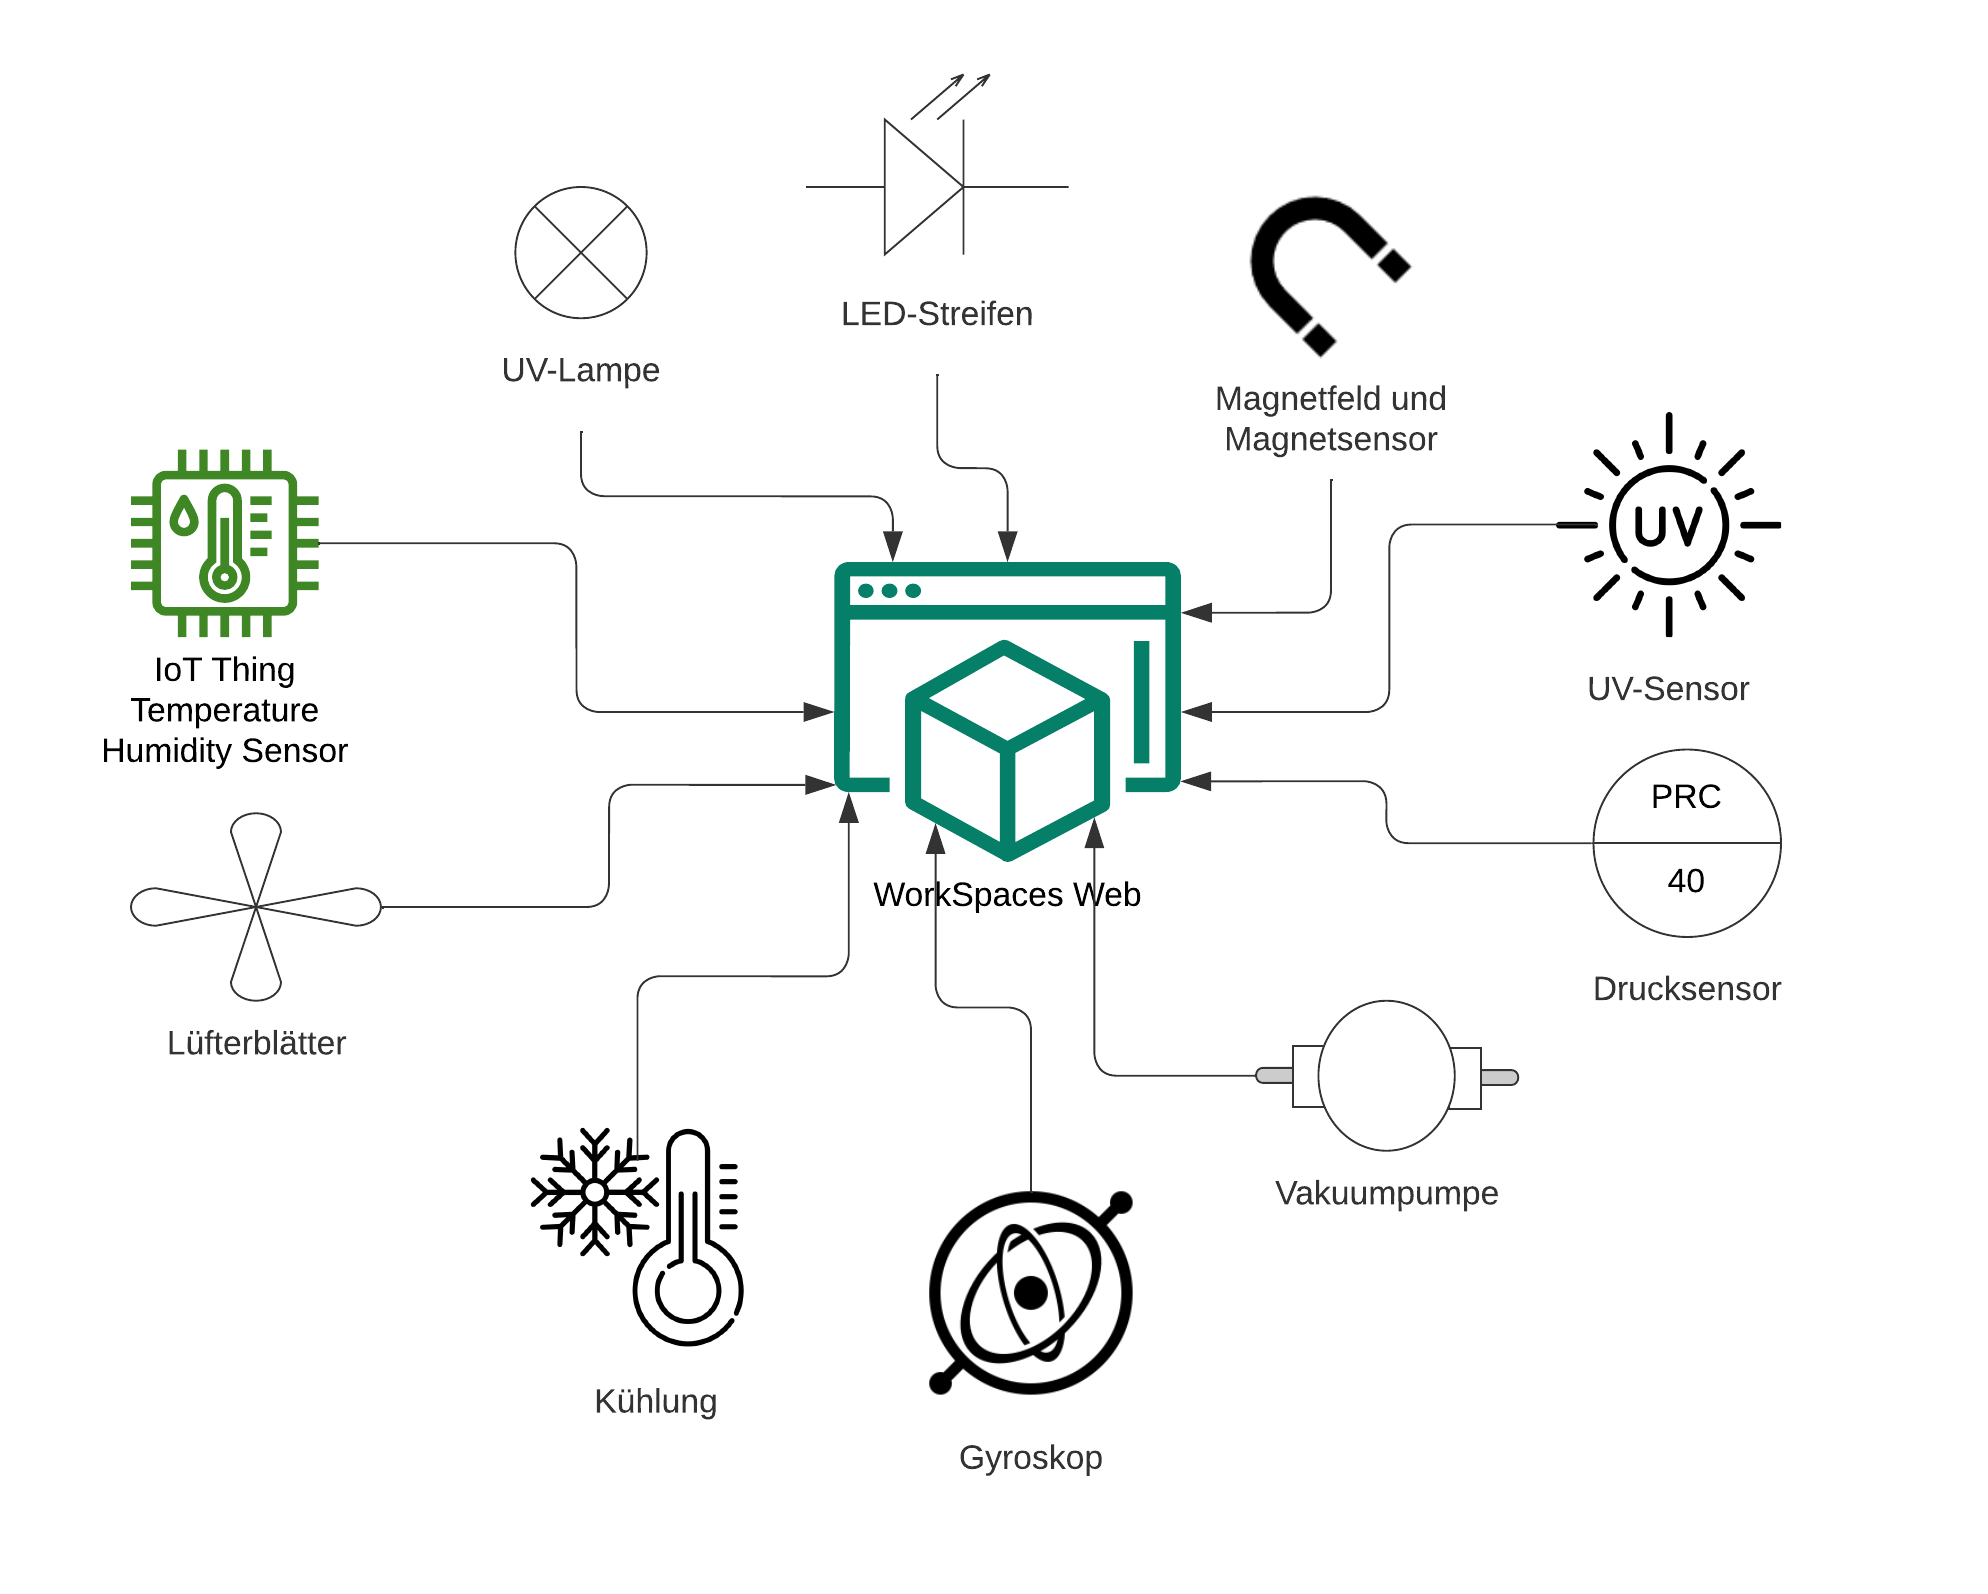
\includegraphics[scale=0.2]{image/blockgesamt.png}
	\caption{Blockschaltbild}
	\label{fig:enter-label}
\end{figure}

Das Setup, mit dem die Teststation gesteuert wird, soll einfach zu bedienen sein. Die Datenauslesung und die Ansteuerung der Geräte sollen in der selben Web-Applikation erfolgen. 
\newpage
\subsubsection{Ziele \textit{Must-Have}}
\begin{itemize}
    \item Rotation des Satellit
    \item Messen der folgenden Auswirkungen auf den CubeSat
    \begin{itemize}
        \item Magnetfeld
        \item Temperatur
        \item UV-Strahlung 
    \end{itemize}
    \item Datenauslesung 
    \item Benutzerfreundliche Bedienoberfläche
\end{itemize}

\subsubsection{Optionale Ziele \textit{Nice-to-Have}}
\begin{itemize}
    \item  Eine Vorrichtung, um ein Vakuum zu erzeugen.
    \item  Auswirkungen von Vibrationen auf den CubeSat
\end{itemize}

\subsection{ Meilensteine}

\begin{table}[h]
    \centering
\begin{tabular}{  l | c | c  } 
  
  \textbf{ Meilenstein} & \textbf{ zu erledigende Arbeit} & \textbf{ bis}\\
  \vspace{2mm}
   \\
   Gehäuse & \parbox{5cm}{Konstuktion und Aufbau des Gehäuses für die Teststation}   & 06.11.2023 \\ 
  \vspace{2mm}
   \\
   Testkammer & \parbox{5cm}{Sensoren einbauen \\ Gyroskop aufbauen \\  Vorrichtung für Vakuum \\ Kühlung \\ UV-Lampe }& 10.02.2024 \\ 
  \vspace{2mm}
   \\
   Daten ein- und auslesen & \parbox{5cm}{Programm für Ein- und Auslesen der Sensoren\\ verschiedene Sendemethoden testen} & 12.02.2024 \\ 
  \vspace{2mm}
   \\
   Limits Testen & Kritische Werte testen & 01.03.2024\\
  \vspace{2mm}
   \\
   Abgabe Diplomarbeit & Dokumentation abgeben & 20.03.2024\\
 
\end{tabular}
    \caption{Meilensteine}
\end{table}
\newpage
\subsection{ Team}
\subsubsection{Teammitglieder}

\begin{figure}[h]
  \centering
  \begin{adjustbox}{valign=c}
    
\includegraphics[scale=0.06]{image/Sophia.jpg}
  \end{adjustbox}
  \hfill
  \begin{minipage}[b]{0.7\textwidth}
    \textbf{\nameSH} \\ 5BHEL
  \end{minipage}
  \captionsetup{justification=raggedright,singlelinecheck=false}
  \caption{\nameSH}
\end{figure}

\begin{figure}[h]
  \centering
  \begin{adjustbox}{valign=c}
    
\includegraphics[scale=0.08]{image/Julius.jpeg}
  \end{adjustbox}
  \hfill
  \begin{minipage}[b]{0.7\textwidth}
    \textbf{\nameJS} \\ 5BHEL
  \end{minipage}
  \captionsetup{justification=raggedright,singlelinecheck=false}
  \caption{\nameJS}
\end{figure}
\newpage
\begin{figure}[h]
  \centering
  \begin{adjustbox}{valign=c}
    
\includegraphics[scale=0.105]{image/consti.jpg}
  \end{adjustbox}
  \hfill
  \begin{minipage}[b]{0.7\textwidth}
    \textbf{\nameCZ} \\ 5BHEL
  \end{minipage}
  \captionsetup{justification=raggedright,singlelinecheck=false}
  \caption{\nameCZ}
\end{figure}

\begin{figure}[h]
  \centering
  \begin{adjustbox}{valign=c}
    
\includegraphics[scale=0.09]{image/Bellai.jpeg}
  \end{adjustbox}
  \hfill
  \begin{minipage}[b]{0.7\textwidth}
    \textbf{\nameSB} \\ 5AHEL
  \end{minipage}
  \captionsetup{justification=raggedright,singlelinecheck=false}
  \caption{\nameSB}
\end{figure}
\newpage
\subsubsection{ Betreungslehrer}
\begin{figure}[h]
  \centering
  \begin{adjustbox}{valign=c}
    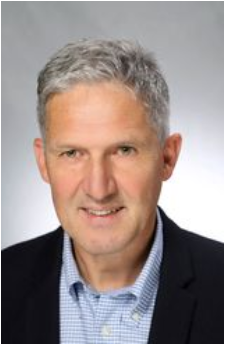
\includegraphics[scale=1]{image/Bischof.png}
  \end{adjustbox}
  \hfill
  \begin{minipage}[b]{0.7\textwidth}
    \textbf{Dipl. Ing. Gerold Bischof} \\ gerold.bischof(at)htl-rankweil.at
  \end{minipage}
  \captionsetup{justification=raggedright,singlelinecheck=false}
  \caption{Diplo. Ing. Gerold Bischof}
\end{figure}

\newpage


\newpage
\input{Abkürzungen}
\newpage
\section{Hardware}
\SecAuth{\nameJS}
\input{Gehäuse}
\newpage
\subsection{Gyroskop}\label{sec:gyroskop}
In der Teststation sollen Tests durchgeführt werden, bei denen sich der Satellit rotiert. Der Satellit sollte sich in alle Richtungen drehen können, denn nur so können die Gyro Sensoren komplett und genau getestet werden. Da sich der Satellit später im All willkürlich rotiert, bringt eine konstante Rotation um nur eine Achse nichts. Aus diesem Grund wird ein sogenanntes Gyroskop oder auch Kreiselinstrument verwendet. Ein Gyroskop kann ein Objekt gleichzeitig in alle Richtungen (x,y,z) drehen. Es besteht aus 3 Ringen, der äußerste Ring wird mit einem Stepper Motor um die X-Achse in Bewegung gesetzt, der Mittlere Ring dreht sich dann mit dem Eigengewicht um die Y-Achse und der innerste Ring ist in unserer Anwendung der Satellit. \\ 
\vspace{3mm}
Um die Ringe in einer Höhe von 30cm zu halten, braucht es 2 Halterungen. Diese Halterungen werden aus Flachstangen, die eine Stärke von 8mm und einer Breite von 20mm haben, geschweißt. Dazu sind folgende Flachstange notwendig. \\
\vspace{3mm}
\begin{table}[H]
    \centering
    \begin{tabular}{ | c | c | } 
  \hline
   \textbf{Bezeichnung} & \textbf{Stückzahl}\\ 
  \hline
   Flachstange 5cm & 4\\ 
  \hline
   Flachstange 20cm & 2 \\ 
  \hline
  Flachstange 25cm & 4 \\ 
  \hline
  Flachstange 10cm & 2 \\ 
  \hline
  Flachstange 30cm & 2 \\ 
  \hline
\end{tabular}
    \caption{Stückliste Halterung Gyroskop}
\end{table}
\vspace{3mm}
\begin{figure}[H]
    \centering
    \begin{subfigure}[b]{0.4\textwidth}
        \centering
        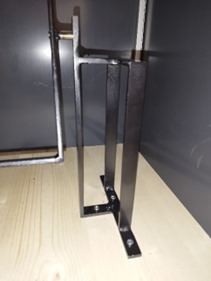
\includegraphics[width=\textwidth]{image/gyroskop1.jpeg}
        
        \label{fig:bild1}
    \end{subfigure}
    \hfill
    \begin{subfigure}[b]{0.4\textwidth}
        \centering
        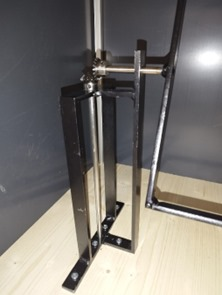
\includegraphics[width=\textwidth]{image/gyroskop2.jpeg}
        
        \label{fig:bild2}
    \end{subfigure}
    \caption{Halterung Gyroskop}
    \label{fig:zwei_bilder}
\end{figure}
\vspace{3mm}

\textbf{Komplette Zusammenschaltung Gyroskop}\\
\vspace{3mm}
Das Relais steuert das Netzteil, welches die Spannung für den Treiber liefert. Der Treiber bekommt Signale vom Raspberry Pi und steuert mit denen die Wicklungen vom Motor. \\
\vspace{3mm}
\begin{figure}[H]
    \centering
    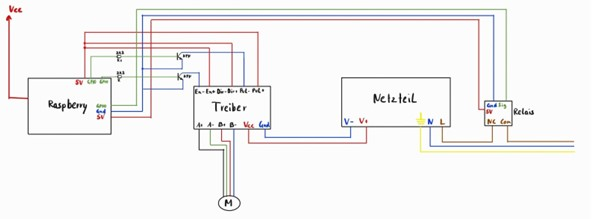
\includegraphics{image/zusammengyros.jpg}
    \caption{Zusammenschaltung Gyroskop}
    \label{fig:enter-label}
\end{figure}


\subsubsection{Motor}
Als Motor wurde der STEPPERONLINE Nema 17 Schrittmotor\autocite{Schrittmotor} gewählt, der speziell für 3D-Drucker und CNC-Reprap-Maschinen konzipiert ist. Mit einem Drehmoment von 59 Ncm, einer Betriebsspannung von 24V, einem Strom von 2A und einem Schrittwinkel von 1.8 Grad pro Schritt gewährleistet er präzise Bewegungssteuerung. Das 4-Draht-Design und das beiliegende 1 Meter lange Kabel mit Verbinder ermöglichen eine einfache Integration in unsere Teststation. Dieser Schrittmotor ist optimal für DIY-Projekte und Anwendungen mit hohen Anforderungen an Präzision und Steuerung von Bewegungen.
\begin{figure}[H]
    \centering
    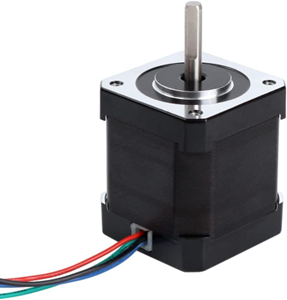
\includegraphics{image/schrittmotor.png}
    \caption{Schrittmotor}
    \label{fig:enter-label}
\end{figure}
Befestigung am Gyroskop und 5V Steuerung FETT:\\
\vspace{3mm}
Zuerst war geplant, den Ring im Gyroskop über eine Antriebsstange zu betreiben, dazu wäre ein 90° Umlenkung mit Zahnrädern notwendig gewesen. Da die Getriebe Stange über 30cm lang ist und nicht präzise zentriert ist, ist es schwierig, ein leicht gängiger Antrieb zu erhalten. Aus diesem Grund wird der Motor direkt an dem Linker Steher befestigt. \\
\vspace{3mm}
\begin{figure}[H]
    \centering
    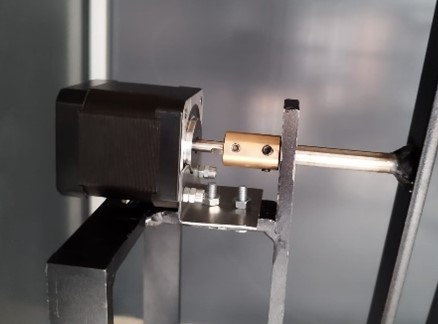
\includegraphics[scale=1.1]{image/motorgyros.jpg}
    \caption{Motor am Gyroskop}
    \label{fig:enter-label}
\end{figure}
\\
\vspace{2mm}
Die GPIO-Pins\label{sec: 5V} vom Raspberry Pi haben eine Ausgangsspannung von 3.3V. Für den Motor Treiber TB6600 wird aber eine Signalspannung von 5V benötigt. Mit einem NPN-Transistor und einem 2k2 Widerstand wird eine Ausgangsspannung von 5V erzeugt. Diese Zusammenschaltung wird auch Emitter Schaltung bezeichnet. Die Basis des bipolaren NPN-Transistors wird über einen Vorwiderstand mit dem Ausgangssignal eines GPIO-Pins vom Raspberry verbunden, während der Emitter mit dem 5V Ausgang vom Raspberry verbunden ist. Am Emitter ist zu gleich das Ausgangssignal mit nun 5V. Dieser wird mit dem Eingang vom Treiber verbunden. 
\subsubsection{Motor-Treiber}
Da man den Motor nicht direkt mit einem Raspberry steuern kann, braucht es einen Motortreiber. Der Twotrees DM542 5.6A Schrittmotortreiber\autocite{Treiber} ist ein leistungsstarker Treiber für 2-Phasen-Schrittmotoren, wie unser Motor, der verwendet wird. Hier ist eine kurze technische Produktbeschreibung:\\
\vspace{3mm}
Eigenschaften:
\begin{itemize}
    \item Leistung: Der Treiber unterstützt Motoren mit bis zu 5.6A Stromversorgung.
    \item Betriebsspannung: Geeignet für Gleichstromquellen im Bereich von 18-48V.
    \item Schrittauflösung: Präzise Mikroschrittsteuerung für genaue Positionierung.
    \item Phasen: Entwickelt für 2-Phasen-Schrittmotoren.
    \item Peak-Strom: Bietet einen Spitzenstrom von bis zu 4.2A für verbesserte Motorleistung.
\end{itemize}
\vspace{3mm}
Schutz und Zuverlässigkeit:
\begin{itemize}
    \item Überstromschutz: Der Treiber ist mit einem Überstromschutz ausgestattet, der den Motor vor Schäden durch zu hohe Ströme schützt.
    \item Wärmeschutz: Integrierter Schutzmechanismus gegen Überhitzung für eine zuverlässige Langzeitnutzung. So können wir die Tests lang genug durchführen.
\end{itemize}
Der Twotrees DM542 5.6A Schrittmotortreiber bietet eine leistungsstarke und zuverlässige Lösung für die Steuerung von 2-Phasen-Schrittmotoren in anspruchsvollen Anwendungen. Mit Funktionen wie Überstromschutz, Wärmeschutz und Mikroschrittsteuerung ist er eine geeignete Wahl für unsere Gyroskop Ansteuerung.
\begin{figure}[H]
    \centering
    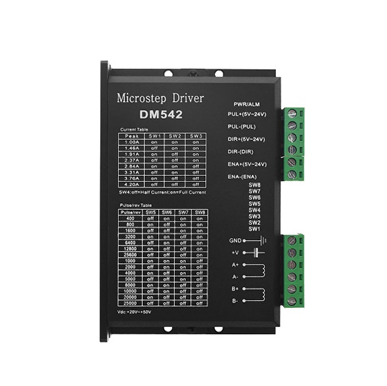
\includegraphics{image/treiber.png}
    \caption{Motor-Treiber}
    \label{fig:enter-label}
\end{figure}

\subsubsection{Netzteil}
Der Motortreiber muss man mit mindestens 9V DC versorgen. Diese Spannung wird mit einem Netzteil erzeugt. Das MeanWell\autocite{MeanWell} LRS-100-24 ist ein industrielles Netzteil mit 108W Leistung, einer Ausgangsspannung von 24V und 4,5A Ausgangsstrom. Es ist für den zuverlässigen Einsatz in industriellen Anwendungen wie Steuerungen und LED-Beleuchtungen konzipiert. Mit integriertem Überlast- und Kurzschlussschutz bietet es eine effiziente und sichere Stromversorgungslösung. Seine robuste Bauweise und Kompaktheit machen es ideal für anspruchsvolle Umgebungen mit begrenztem Platz.
\vspace{5mm}
\begin{figure}[H]
    \centering
    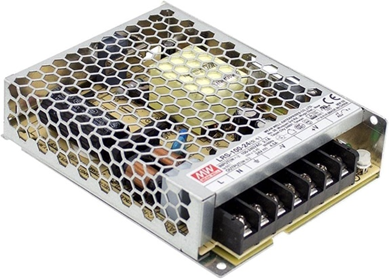
\includegraphics{image/Netzteil.png}
    \caption{Netzteil}
    \label{fig:enter-label}
\end{figure}

\newpage
\subsubsection{Relais}\label{sec:relai}
\begin{figwindow}[1,r,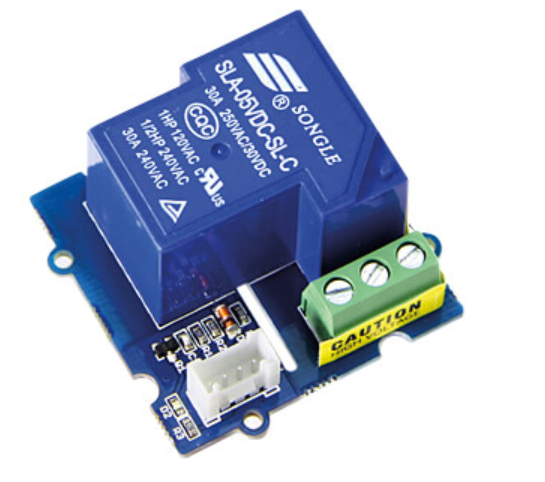
\includegraphics[scale=0.5]{image/relai.jpg.png},{Relais\autocite{Relais}}]
Mit einem Relais kann man mit kleinen Spannungen große Spannungen schalten. Ein Relais\autocite{Relais} besteht aus einer Spule und einem beweglichen Kontakt. Wenn Strom durch die Spule fließt, erzeugt sie ein Magnetfeld, das den Kontakt beeinflusst. Dadurch ändert sich der Zustand des Schaltkontakts, und ein elektrischer Pfad wird geöffnet oder geschlossen. Relais dienen dazu, mit einem schwachen Steuersignal einen starken elektrischen Stromkreis zu steuern oder zu schalten. Relais werden in unserer DA verwendet, um mit dem Raspberry Netzspannungen zu schalten. 
Für unsere Anwendung brauchen wir das GRV RELAY SPDT30, dieses ist ein hochwertiges einpoliges Zweiwege-Relais mit hoher\\ Schaltleistung. Es ist für Betriebsspannungen von 4,75 bis 5,25 V und Schaltströme von bis zu 30 A bei 250 V AC oder 30 V DC ausgelegt. Das Relais ist kompatibel mit den Schnittstellen vom Raspberry Pi, verfügt über eine schnelle Einschaltzeit von maximal 15ms und eine Betriebstemperatur von -25 bis +75°C.  Eingesetzt wird es in der Teststation für die Steuerung des Netzteils und für die UV Lampe.
\end{figwindow}

\newpage
\SecAuth{\nameSH}
\subsection{Leiterplatte}
In dieser Anwendung ist die Leiterplatte ein Raspberry Shield. Ein Shield sorgt dafür das alle Komponenten, die angesteuert werden sollen, übersichtlich an den \raspi angeschlossen werden. Es kann aber auch sein, dass das Shield eine Erweiterung für den \raspi ist.
In diesem Fall wurde das Shield verwendet, um die Komponenten mit dem \raspi zu verbinden.\\
\vspace{3mm}
PCB und der Schaltplan wurden in Eagle 7.0.0 entworfen.
\subsubsection{Schaltplan}
Das Shield wird über den PRT-14017\autocite{PRT-14017} Header mit dem \raspi verbunden\\
\vspace{3mm}
\begin{figure}[H]
\centering
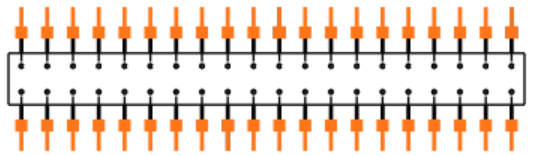
\includegraphics[scale=0.7]{image/prt140117.png}
\caption{Schaltplansymbol PRT-14017}
\end{figure}
Um die verschiedenen Komponenten anzuschließen, werden Schraubklemmen verwendet. Es werden fünf 4-Polige Schraubklemmen\autocite{4-polige-Schraubklemme} und elf 3-Polige Schraubklemmen\autocite{W237-103} benötigt.\\
\vspace{3mm}
Nachdem die Schraubklemmen und der Header platziert wurden, werden die Pole der Schraubklemmen mit dem Header verbunden. Die Zuordnung ist in der Tabelle 7 zu sehen. \\
\vspace{3mm}
\begin{table}[h]
    \centering
    \begin{tabular}{ | c | c | c | c | } 
  \hline
  \textbf{ Bezeichnung} & \textbf{ GPIO-Pin} & \textbf{ GPIO-Pin} & \textbf{ Versorgung}\\
  \hline
   Lüfter & GPIO19 & - & -  \\ 
  \hline
    Kühlung & GPIO12 & - & 5V  \\ 
  \hline
   LED-Streifen & GPIO20 & GPIO21 & - \\ 
  \hline
   Schlüsselschalter & GPIO06 & - & 3.3V \\ 
  \hline
   Ventil2 & GPIO25 & - & 5V \\
  \hline
   Notaus & GPIO05 & - & 3.3V \\
  \hline
   Ventil1 & GPIO24 & - & 5V \\
  \hline
   UV-Lampe & GPIO18 & GPIO23 & 5V \\
  \hline
   Endschalter & GPIO27 & GPIO22 & 5V \\
  \hline
   Motor & GPIO17 & GPIO13 PWM & - \\
  \hline
   Netzteil & GPIO14 & GPIO15 & 5V \\
  \hline
   Temperatursensor1 & GPIO07 & - & 5V \\
  \hline
   Temperatursensor2 & GPIO08 & - & 5V \\
  \hline
   Magnetsensor & GPIO16 & - & 3.3V \\
  \hline
   Drucksensor & GPIO03 SDA & GPIO05 SCL & 5V \\
  \hline
   UV-Sensor & GPIO03 SDA & GPIO05 SCL & 5V \\
  \hline
\end{tabular}
    \caption{Pinbelegung \raspi Shield}
\end{table}
\newpage
Der Drucksensor und der UV-Sensor sind beide über die I2C-Schnittstelle mit dem Raspberry Shield verbunden.\\
\vspace{3mm}
Information über die I2C-Schnittstelle sind unter \url{https://www.ti.com/lit/an/slva704/slva704.pdf?ts=1712280198725&ref_url=https%253A%252F%252Fwww.google.com%252F} zu finden.\\

\newpage
\begin{figure}[h]
\centering
    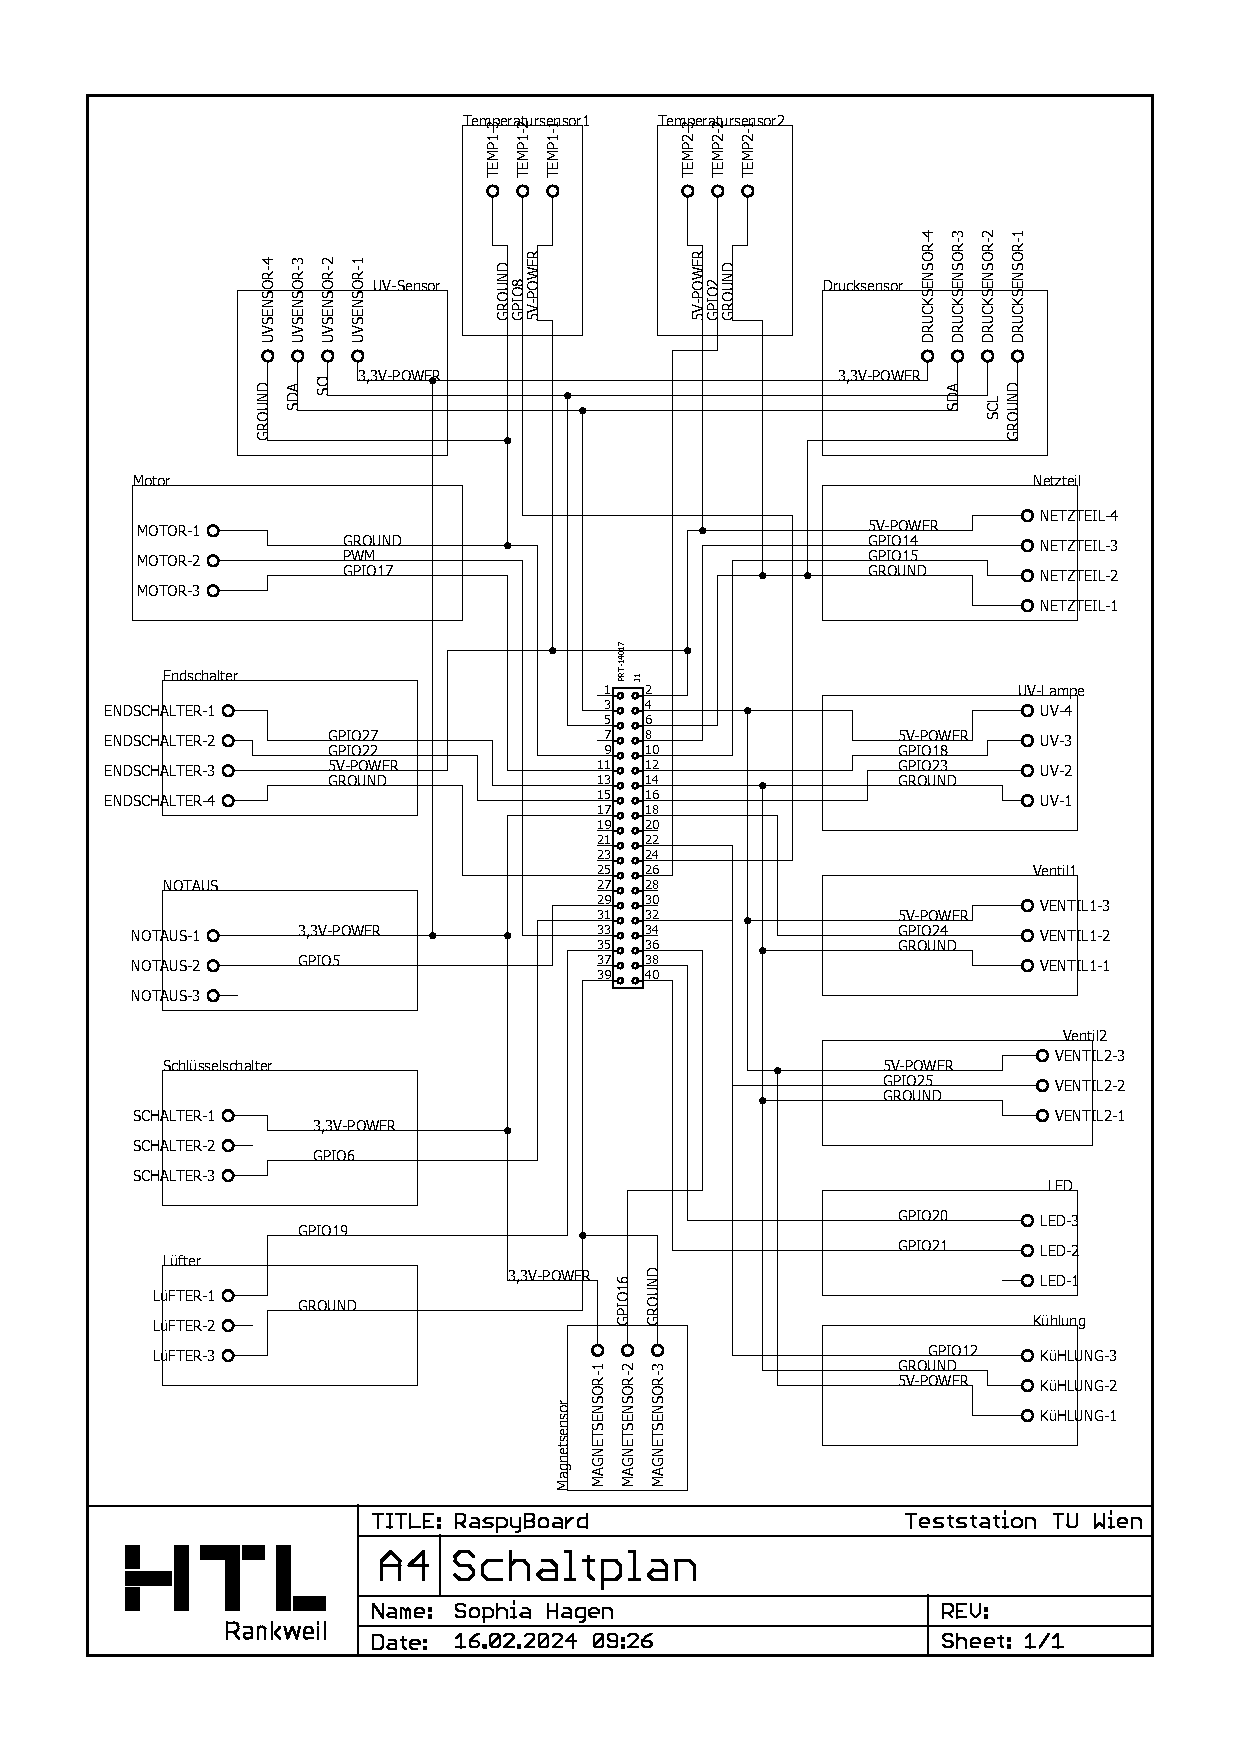
\includepdf[pages=1]{pdf/RaspyBoard_Schematic}
    %\caption{Schaltplan}
\end{figure}
\pagebreak
\subsubsection{PCB}
Die Platine hat eine Größe von \textit{95mm X 65mm}. Geplant war, das Board in der Größe des \raspi zu entwerfen. Der \raspi 4B besitzt 2 USB-Buchsen und und ein LAN-Anschluss. Diese sind jedoch zu hoch, um darüber eine Platine zu platzieren die mit dem \raspi verbunden werden soll. Aus diesem Grund wurde das Board in die Länge gezogen. Die 16 Schraubklemmen werden einzeln beschriftet. Beispielsweise hat die Schraubklemme für den UV-Sensor die Beschriftung UV-Sensor. Zur Befestigung werden 4 Bohrungen benötigt. Diese haben einen Durchmesser von \textit{3.5mm}.\\
\vspace{3mm}
\begin{figure}[H]
	\centering
	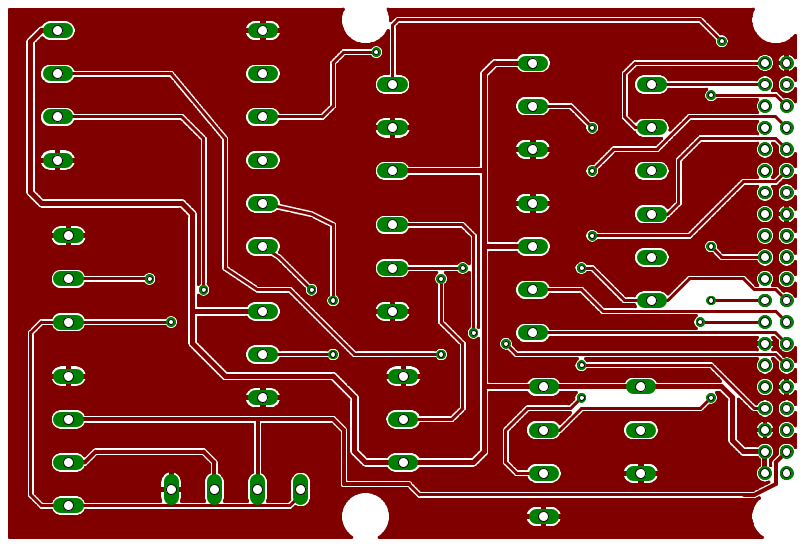
\includegraphics[scale=0.8]{image/layouttop.png}
	\caption{Layout Top}
	\label{fig:enter-label}
\end{figure}
\begin{figure}[H]
	\centering
	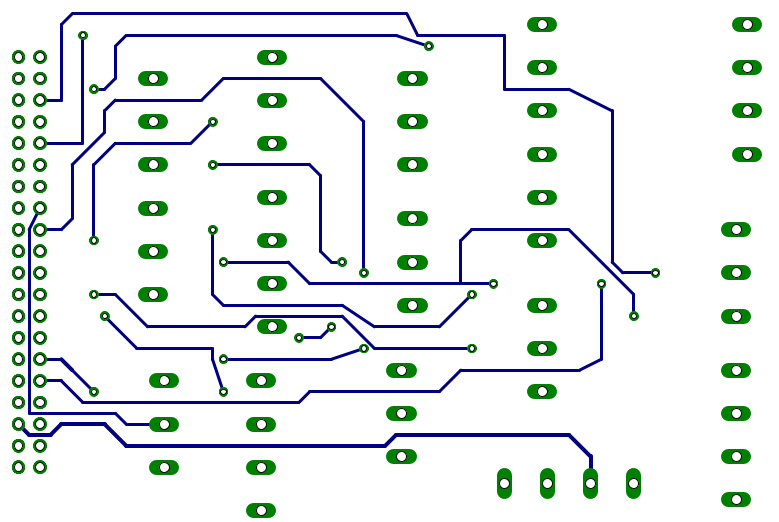
\includegraphics[scale=0.8]{image/layoutbottom.png}
	\caption{Layout Bottom}
	\label{fig:enter-label}
\end{figure}
\newpage
\begin{figure}[H]
	\centering
	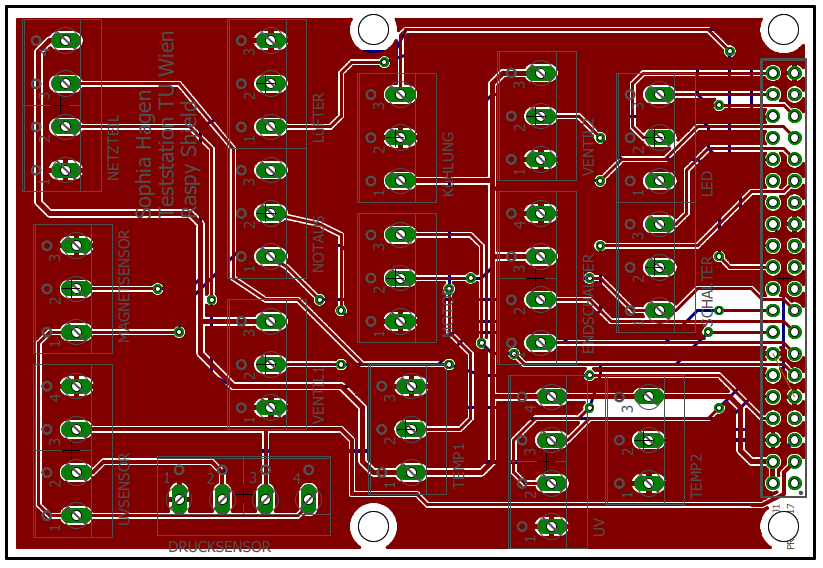
\includegraphics[scale=0.8]{image/workp.png}
	\caption{PCB mit Polygon}
	\label{fig:enter-label}
\end{figure}
\begin{figure}[H]
	\centering
	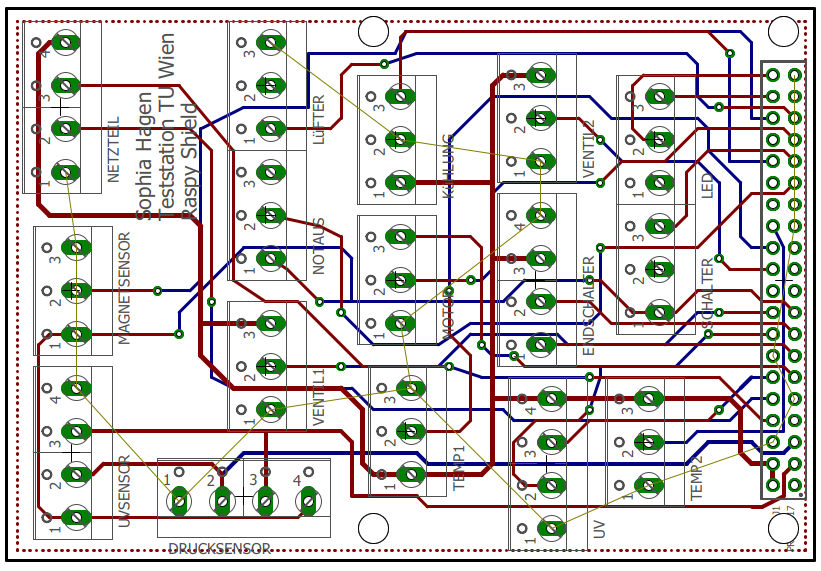
\includegraphics[scale=0.8]{image/worko.png}
	\caption{PCB ohne Polygon}
	\label{fig:enter-label}
\end{figure}
\pagebreak
\begin{figure}[H]
\centering
    \includegraphics[scale=0.27]{image/Platine_unbestückt.jpg}
    \caption{Unbestückte Platine}
\end{figure}
\begin{figure}[H]
\centering
    \includegraphics[scale=0.18]{image/platine_bestückt.jpg}
    \caption{Bestückte Platine}
\end{figure}
\newpage
\subsection{Sensoren in der Testkammer}\label{sec:Sensoren in der Testkammer}
Die verschiedenen Sensoren werden in der Testkammer platziert, damit einen Vergleich zwischen den Sensorwerten in der Kammer und auf dem CubeSat dargestellt werden kann. Dieser Vergleicht ist eine Überprüfung, ob alle Sensoren auf dem CubeSat noch funktionieren und richtige Werte ausgeben. Bei den verwendeten Sensoren musste darauf geachtet werden, dass sie bei einer Temperatur von 0°C bis 30°C betrieben werden können.
\begin{figure}[H]
	\centering
	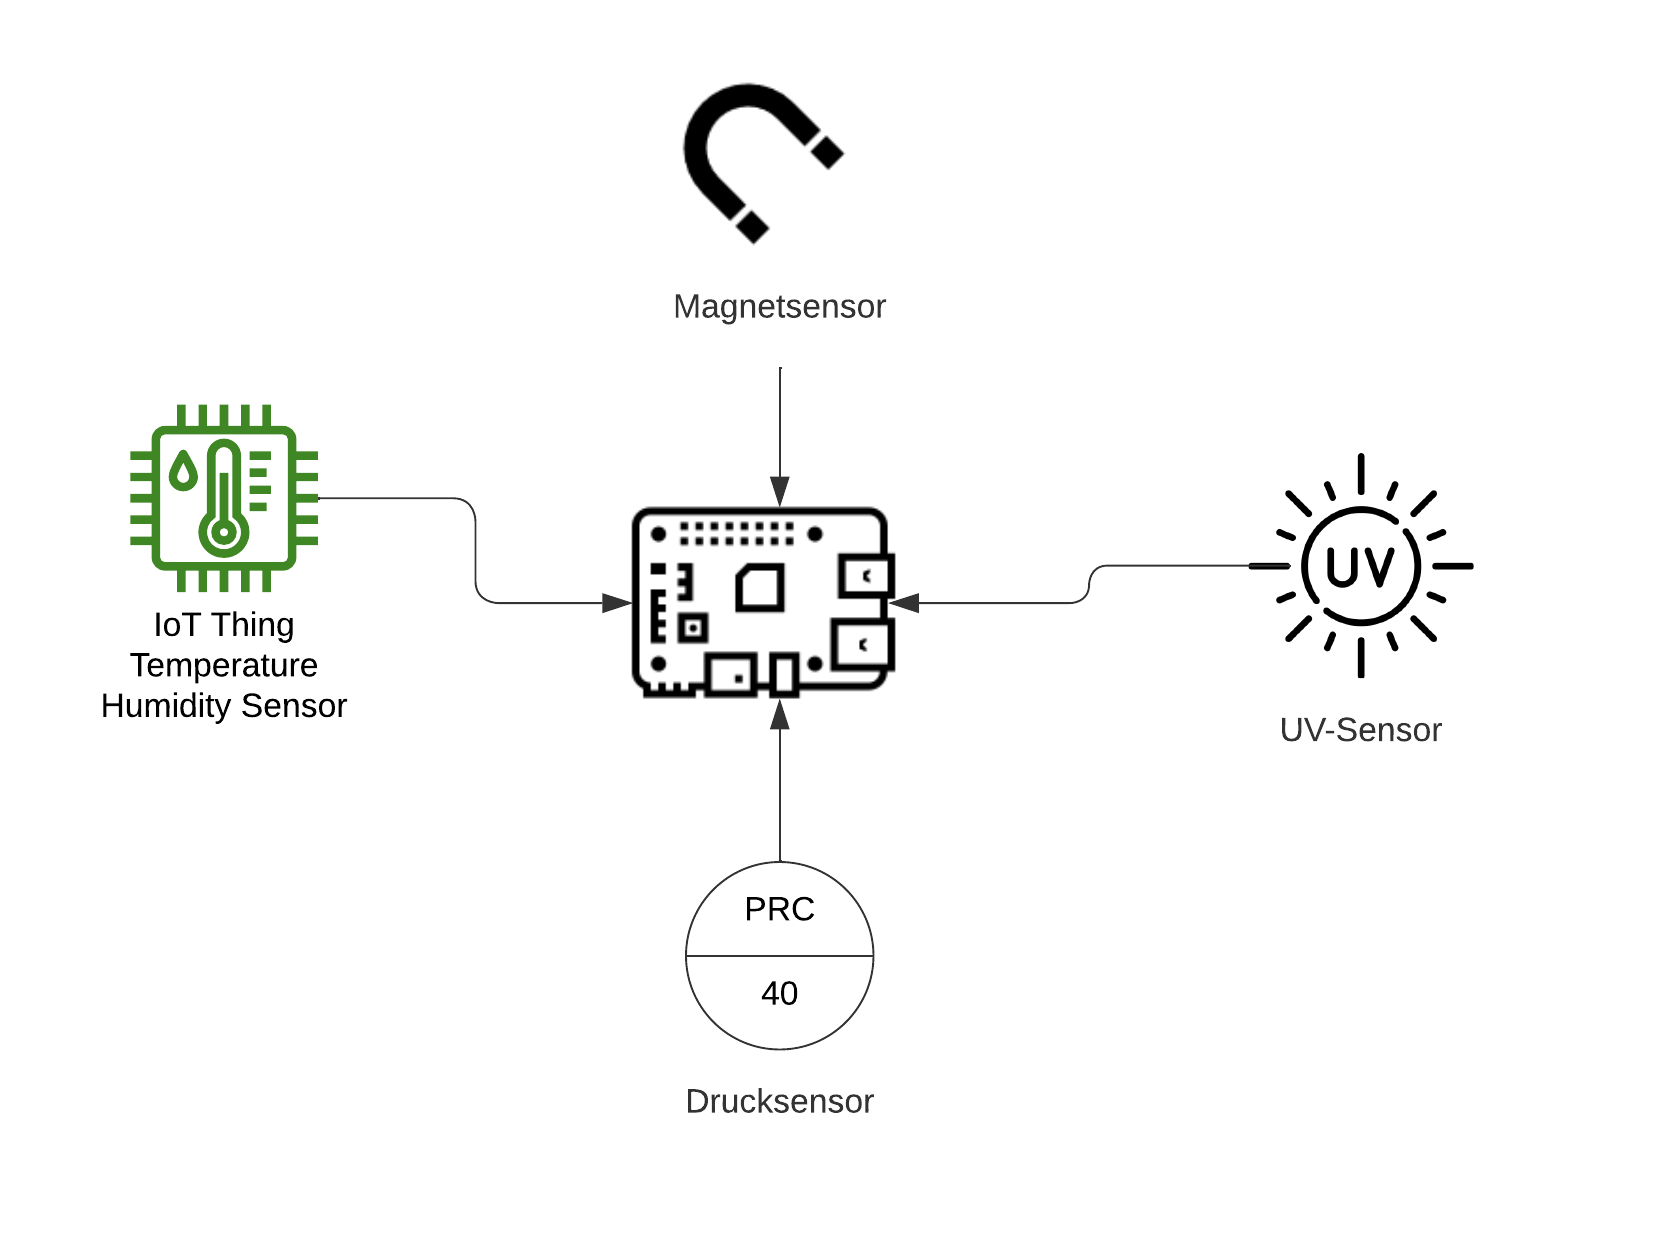
\includegraphics[scale=0.3]{image/blocksensor.png}
	\caption{Blockschaltbild Sensoren}
\end{figure}

\newpage
\subsubsection{Temperatursensor}\label{sec:Temperatursensor}
In der Testkammer befinden sich zwei Temperatursensoren mit integriertem Feuchtigkeitssensoren. Diese messen die Temperatur sowie die Feuchtigkeit in der Kammer. Dadurch können die Sensorwerte der Kammer und des CubeSat verglichen werden.\\
\vspace{3mm}
Für diese Anwendung wird der Temperatursensor \textbf{AM2302} \autocite{AM2302} verwendet. Der Anschluss an den \raspi erfolgt durch die PCB. Der Sensor wird mit 3 Pins an die PCB angeschlossen.\\
\vspace{3mm}
\begin{table}[H]
    \centering
    \begin{tabular}{ | c | c | } 
  \hline
   VDD & 5 Volt\\ 
  \hline
   GND & Ground\\ 
  \hline
   Data & GPIO7 und GPIO8\\ 
  \hline
\end{tabular}
    \caption{Pinbelegung Temperatursensor}
\end{table}
Um beide Sensoren in der Testkammer zu montieren, wurde ein Gehäuse in SolidWorks entworfen. Danach wurden die Teile mit dem 3D-Drucker ausgedruckt.\\
\vspace{2mm}
\begin{figure}[H]
\centering
\includegraphics[scale=0.6]{image/Gehäusetemp.png}
\caption{Gehäuse Temperatursensor}
\end{figure}
\newpage
Um den Temperatursensor zu verwenden, wird eine Bibliothek benötigt. Die Bibliothek wird von Adafruit bereitgestellt. Um diese zu installieren wird folgender Befehl auf dem \raspi ausgeführt:\\
\begin{verbatim}
pip3 install adafruit-circuitpython-dht
\end{verbatim}
Durch die Bibliothek\autocite{Adafruit_DHT} wird das Auslesen des Sensors vereinfacht. Mit wenigen Befehlen kann der Sensor die Temperatur und die Feuchtigkeit messen.\\
\vspace{3mm}
\begin{figure}[H]
    \centering
    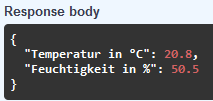
\includegraphics[scale=1.5]{image/Tempausgabe.png}
    \caption{Temperatursensorausgabe}
    \label{fig:enter-label}
\end{figure}
Die Messung mit dem Temperatursensor wurden in einem normalen Zimmer mit Raumtemperatur durchgeführt. Die ermittelten Daten für Temperatur und Feuchtigkeit werden in der oberen Abbildung abgebildet.\\
\vspace{3mm}
Die Programmierung für das Testprogramm befindet sich im Kapitel \ref{sec:Testprogramm Temp}, und der Programm Abschnitt für die API im Kapitel \ref{sec:API-Temp}





\subsubsection{UV-Sensor}
Der CubeSat besitzt einen UV-Sensor, aus diesem Grund wurde auch in die Testkammer einer eingebaut. Es wurde der UV-Sensor LTR390\autocite{LTR390} verwendet. Dieser verfügt über einen integrierten ADC, somit muss kein Analog-Digital-Wandler dazwischengeschaltet werden und kann direkt über I2C an den \raspi angeschlossen werden.\\
\vspace{5mm}
\begin{table}[H]
    \centering
    \begin{tabular}{ | c | c | } 
  \hline
   VCC & 5 Volt\\ 
  \hline
   GND & Ground\\ 
  \hline
   SDA & GPIO3 \\ 
  \hline
   SCL & GPIO5 \\ 
  \hline
   INT & Interruptausgang \\ 
  \hline
\end{tabular}
    \caption{Pinbelegung UV-Sensor}
\end{table}
\begin{figwindow}[0,r,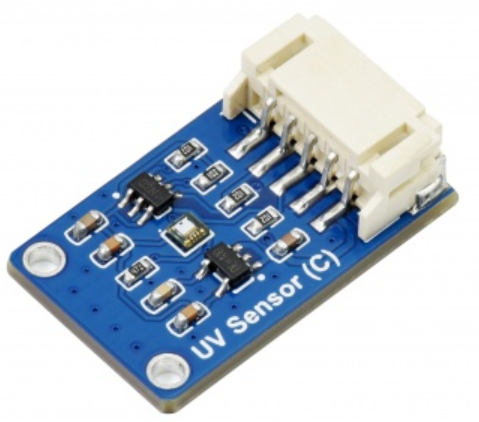
\includegraphics[scale=0.5]{image/UVsensor.png},{UV-Sensor}]
Das Licht der UV-Lampe\ref{sec:UV-Lampe} hat eine Wellenlänge von 385nm bis 400nm. Daher muss der UV-Sensor auch für diesen Bereich ausgelegt sein. Der Messbereich des LTR390 ist zwischen 200nm und 400nm. Der Sensor misst das Umgebungslicht und den UV-Index. Das Umgebungslicht wird in Lux angegeben. Ein niedriger Lux-Wert bedeutet das der Sensor sich in einer dunklen Umgebung befindet. Ein hoher Wert bedeutet eine helle Umgebung. Der UV-Index wird in verschiedene Kategorien eingeteilt.
\end{figwindow}
\vspace{2mm}
\begin{table}[h]
    \centering
    \begin{tabular}{ | c | c | } 
  \hline
   UV-Index & Kategorie\\ 
  \hline
   0-2 & Niedrig\\ 
  \hline
   3-5 & Mäßig \\ 
  \hline
   6-7 & Hoch \\ 
  \hline
   8-10 & sehr Hoch \\ 
  \hline
   11+ & Extrem \\ 
  \hline
\end{tabular}
    \caption{UV-Index}
\end{table}

\begin{figure}[H]
    \centering
    \begin{subfigure}[b]{0.45\textwidth}
        \centering
        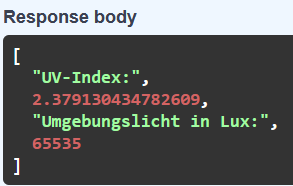
\includegraphics[width=\textwidth]{image/UVsensor hell.png}
        \caption{indirektes Sonnenlicht}
        \label{fig:bild1}
    \end{subfigure}
    \hfill
    \begin{subfigure}[b]{0.45\textwidth}
        \centering
        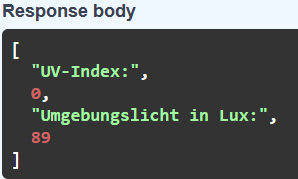
\includegraphics[width=\textwidth]{image/uvsensor dunkel.png}
        \caption{kein Sonnenlicht}
        \label{fig:bild2}
    \end{subfigure}
    \caption{Messungen mit UV-Sensor}
    \label{fig:zwei_bilder}
\end{figure}
Die Messungen der oberen zwei Abbildungen wurden in einem Zimmer durchgeführt. Der Sensor in Abbildung (a) wurde für die Messung dem Sonnenlicht durch ein Fenster ausgesetzt. Aus diesem Grund ist der UV-Index eher niedrig. Der LTR390 kann Umgebungslicht von 0 Lux bis zu 65535 Lux messen. In Abbildung (a) ist zu erkennen, dass der maximale Wert bei der Messung des Umgebungslichtes erreicht wurde. Daraus kann geschlussfolgert werden, dass sich der Sensor in einer hellen Umgebung befunden hat. In Abbildung (b) wurde der Sensor vom Sonnenlicht entfernt, somit haben keine UV-Strahlen den Sensor getroffe. Dies kann auch am gemessenen UV-Index erkennt werden. Es wurde ein Umgebungslicht von 89 Lux gemessen. Der UV-Sensor war also in einer eher dunklen Umgebung.\\
Für den LTR390 UV-Sensor wird die folgende Bibliothek\autocite{LTR390} verwendet:
\begin{verbatim}
pip install adafruit-circuitpython-ltr390
\end{verbatim}
\vspace{3mm}
Das Testprogramm für den UV-Sensor ist im Kapitel \ref{sec:Testprogramm UV-Sensor} und der Codeabschnitt für die API im Kapitel \ref{API-UVS}
\subsubsection{Magnetsensor}\label{sec: Magnetsensor}
Der Magnetsensor misst das Magnetfeld in seiner Umgebung. Der KY-024 Linearer, magnetischer Hall-Sensor\autocite{KY-024}, ist für den Dauerbetrieb geeignet und ist in einem Temperaturintervall von -150°C bis 150°C stabil. \\
\vspace{3mm}
\begin{figure}[H]
    \centering
    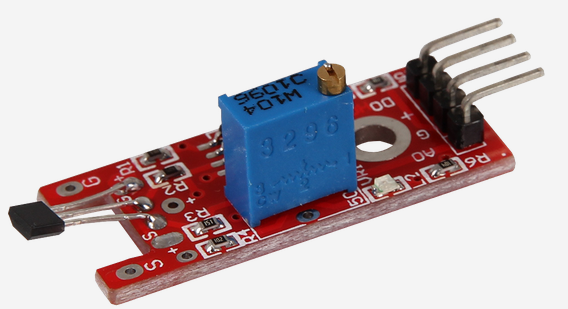
\includegraphics[scale=0.8]{image/magnetsensir.png}
    \caption{KY-024 Magnetsensor}
    \label{fig:enter-label}
\end{figure}
\vspace{3mm}
Der Sensor besitzt zwei LEDs. 
\begin{itemize}
    \item LED 1: zeigt an, ob der Sensor mit Strom versorgt wird.
    \item LED 2: zeigt an, ob der Sensor ein Magnetfeld erkannt hat.
\end{itemize}
\vspace{3mm}
Durch ein Drehpotentiometer kann die Empfindlichkeit des Sensors eingestellt werden. Über den digitalen Ausgang des Sensors wird ein Signal ausgegeben, sobald ein Magnetfeld erkannt wird.\\
\newpage
Der KY-024 ist ein analoger Sensor. Da der \raspi keinen integrierten ADC besitzt, muss einer gekauft werden, damit der Sensor über den \raspi angesteuert und gelesen werden kann. Als ADC eignet sich hierfür der 16-Bit ADC KY-053\autocite{KY-053}. \\
\vspace{2mm}
\textbf{Zusammenschaltung von \raspi, Magnetsensor und ADC}
\begin{figure}[H]
    \centering
    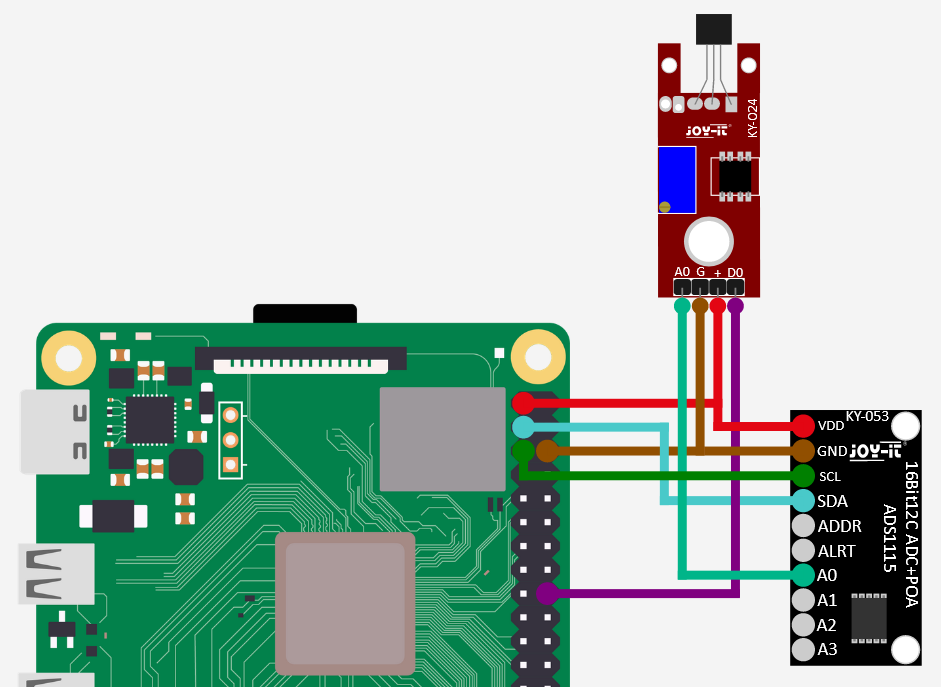
\includegraphics[scale=0.6]{image/zusammenmanet.png}
    \caption{Zusammenschaltung Magnetsensor\autocite{Zusammenschaltungmagnet}}
    \label{fig:enter-label}
\end{figure}
\subsubsection{Drucksensor}
In der Teststation gibt es eine Vorrichtung, um ein Vakuum zu erzeugen. Durch dieses Vakuum kann der integrierte barometrischer Drucksensor auf dem CubeSat getestet werden. Der Drucksensor in der Kammer wird dazu verwendet, einen Vergleich zwischen Testkammer und Satellit herzustellen.\\
\vspace{3mm}
Es wurde der Drucksensor BMP180\autocite{BMP180} verwendet. Er befindet sich in der Testkammer, hat jedoch keinen fixen Platz. Der Sensor kann je nachdem, ob ein Vakuum erzeugt wird oder nicht, platziert werden. Der BMP180 hat 4 Pins die über die PCB angeschlossen und mit dem \raspi verbunden. werden.\\
\vspace{3mm}
\begin{table}[h]
    \centering
    \begin{tabular}{ | c | c | } 
  \hline
   Vin & 5 Volt\\ 
  \hline
   GND & Ground\\ 
  \hline
   SDA & GPIO3 \\ 
  \hline
   SCL & GPIO5 \\ 
  \hline
\end{tabular}
    \caption{Pinbelegung Drucksensor}
\end{table}
\vspace{3mm}
Um den Sensor verwenden zu können, muss auch hier eine Bibliothek heruntergeladen werden. Diese wird von Adafruit bereitgestellt. Mit folgendem Befehl kann die Bibliothek\autocite{BMP180bib} heruntergeladen werden.
\begin{verbatim}
pip install circuitpython-bmp180
\end{verbatim}
Die Suche nach einer geeigneten Bibliothek war nicht einfach, da die meisten Repository archiviert wurden. In einigen Dokumenten wird auch angegeben, dass der Drucksensor BMP180 gar nicht mehr hergestellt wird.\\
\vspace{3mm}
\begin{figure}[H]
    \centering
    \begin{subfigure}[b]{0.7\textwidth}
        \centering
        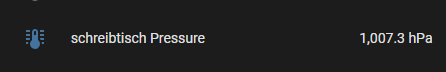
\includegraphics[width=\textwidth]{image/druckvergleich.png}
        \caption{Messung über Wetterstation}
        \label{fig:bild1}
    \end{subfigure}
    \hfill
    \begin{subfigure}[b]{0.5\textwidth}
        \centering
        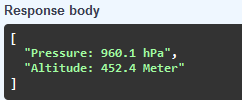
\includegraphics[width=\textwidth]{image/druckausgabe.png}
        \caption{Messung mit Drucksensor}
        \label{fig:bild2}
    \end{subfigure}
    \caption{Druckmessungen}
    \label{fig:zwei_bilder}
\end{figure}
Die oben angeführten Druckmessungen, wurden beide in Wolfurt durchgeführt. Der Druck in Abbildung (a), wurde mit einer Netatmo Wetterstation\autocite{Netatmo} gemessen. In Abbildung (b), wurde der BMP180 Drucksensor verwendet, um den Druck zu ermitteln. Die Werte stimmen einigermaßen überein. Auch die Meereshöhe kann mit dem BMP180 angezeigt werden. Wolfurt liegt auf einer Meereshöhe von 434 m. Der Sensor zeigt eine Meereshöhe von 452 Metern an. Da dieser Wert nicht genau mit dem tatsächlichen Wert über einstimmt, kann eine Kalibrierung durchgeführt werden. Dies erfolgt durch eine Anpassung an der Berechnung im Code.\\
\vspace{3mm}
Der Codeabschnitt für das Testprogramm befindet sich im Kapitel  \ref{sec:Testprogramm Drucksensor}. Das Programm für die API ist im Kapitel \ref{sec:API-Druck}.
\newpage
\SecAuth{\nameCZ}
\newpage
\subsection{Sensoren auf dem Satellit}\label{sec:sensoraufcube}

\subsubsection{EDU}\label{edu}
Die Programmierung des EDU (Educational Module), welches sich im Cubesat der TU-Wien befindet, dient als eine Plattform, welche für Schülerinnen und Schüler zur Verfügung steht, um über ihre Software verschiedene Experimente durchzuführen. Das Modul besteht aus einem Raspberry PI, verschiedenen Sensoren und zwei Kameras (siehe Abb.), welche beide genutzt werden können. Die Ansteuerung der Sensoren funktioniert über den I2C-Bus. \\
\vspace{4mm}
\begin{figure}[H]
    \centering
    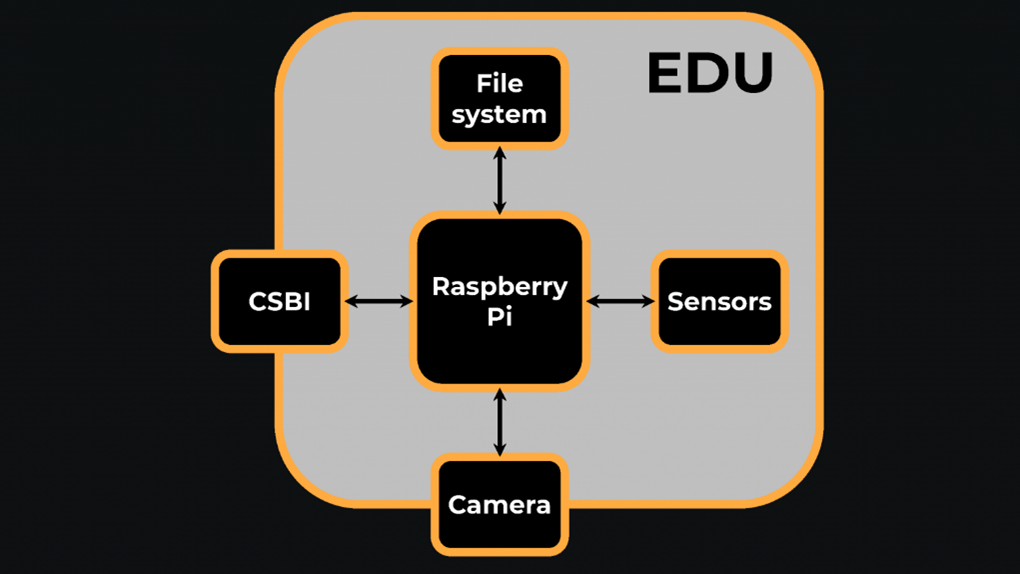
\includegraphics[scale = 0.8]{image/blockschaltnildedu.png}
    \caption{Blogschaltbild des EDUs}
    \label{fig:enter-label}
\end{figure}
\vspace{1mm}
Das System kann von jeder Person zuhause getestet werden. Dazu dient der EDU-Hat, eine Platine, welche die Sensorik des EDUs enthält und sich einfach auf einen Raspberry PI stecken lässt.
\newpage
\subsubsection{Sensorik des EDUs}
Auf dem EDU sind folgende Sensoren zu finden: 
\begin{itemize}
    \item Temperatursensor 
    \item Magnetfeldsenso
    \item Beschleunigungssensor
    \item Gyroskop
    \item GNSS-Empfänger
    \item UV-Sensoren
    \item Dosimeter
\end{itemize}
Der verwendete EDU-HAT (Simulation des EDUs für Selbstexperimente auf dem Boden) besitzt jedoch nur einen Temperatursensor, einen Beschleunigungssensor, einen Magnetfeldsensor, einen UV-Sensor und einen Gas Sensor. Die Montage einer Raspberry PI Kamera ist jedoch auch möglich.\\

\subsubsection{Temperatursensor}\label{temperatur}
Sowohl auf dem EDU-Hat als auch auf dem EDU selbst befinden sich 2 Sensoren, welche Temperaturen messen können. \\
\vspace{3mm}
Der Sensor TMP112\autocite{TMP112} ist ein rein digitaler Temperatursensor, welcher im Bereich von -40°C bis 125°C akkurat (±0,5°C bei 0° bis 65°C und ±1°C bei -40 bis 125°C) Temperaturen messen kann. Die Betriebsspannung des Sensors liegt bei 1.4V-3.3V bei einem maximalen Strom von 10µA. \\
\vspace{3mm}
Der Gas Sensor BME688\autocite{BME688} dient als Feuchtigkeitssensor, Gassensor und als guter Temperatursensor. Auch ist die Messung des Luftdrucks möglich. Die Betriebsspannung des Sensors liegt zwischen 1.71V-3.6V, während der Sensor je nach Betriebsmodus zwischen 2,1µA und bis zu 0,9mA Strom verbraucht. Der Arbeitsbereich des Sensors liegt zwischen -40°C bis 85°C für die Temperatur, 0-100°C für Luftfeuchtigkeit und Gaserkennung und 300-1100 hPa für den Luftdruck. 

\subsubsection{Magnetfeldsensor/Gyroskop}\label{magentsen}
Der BMM150\autocite{BMM150} ist ein dreiachsiger geomagnetischer Sensor, welcher sich für die Messung von Magnetfeldern und deren Einwirkungen eignet. Der Arbeitsbereich des Sensors liegt zwischen -40°C bis +85°C bei einer Betriebsspannung von 1.62V-3.6V. Auch der Stromverbrauch ist bei 170µA minimal. Die Rückgabe des Sensors besteht aus X, Y und Z Werten, welche die Stärke des Magnetfeldes in den verschiedenen Richtungen darstellen. 

\subsubsection{Beschleunigungssensor}\label{beschleuni}
Der Beschleunigungssensor ADXL345\autocite{ADXL345} dient als dynamischer Sensor, indem er Bewegung und Schock in G-Kräften zurückgibt. Der wichtigere Messbereich des ADXL345 Sensors ist die statische Messung, welche die Gravitation auf den verschiedenen Achsen zurückgibt. Aus dieser Information heraus kann der Winkel des Sensors ausgerechnet werden und somit als Gyroskop Sensor verwendet werden. \\
\vspace{3mm}
Der Stromverbrauch des Sensors liegt bei 40µA bei einer Betriebsspannung von 2.0V bis 3.6V. Der Sensor hat eine Auflösung von 13-Bit und misst in den Bereichen von ±16g, was umgerechnet rund ±156,91 m/s² entspricht. \\
\vspace{3mm}
Die Rückgabewerte des Beschleunigungsmessers entsprechen den G-Kräften an den X, Y- und Z-Achsen.

\subsubsection{UV-Sensor}\label{uvsens}
Der UV-Sensor GUVA\_C32 dient zur Messung von UV-Strahlen welche sich im Orbit, bzw. auf dem Boden befinden. UV-Strahlungen werden in Stärkegraden\autocite{Cosmic} als UV-Index (1-14 UV) angegeben. Die Betriebsspannung des Sensors liegt zwischen 2.6V bis 3.6V bei einem Stromverbrauch von 100µA.  

\subsubsection{Dosimeter}\label{dosimet}
Der Dosimeter ist einer der Sensoren, welche auf der EDU-Hat nicht vorhanden sind. Seine Aufgabe ist es ionisierte Strahlung zu empfangen. Strahlungen dieser Art sind hauptsächlich in höheren Elevationen verbreitet (siehe Abb. 40).\\
\vspace{3mm}
\begin{figure}[H]
    \centering
    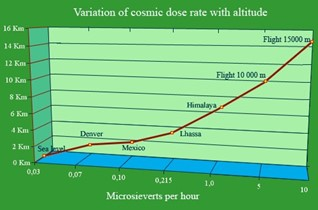
\includegraphics[scale=1.2]{image/bilduv.jpg}
    \caption{Korrelation Dosimeter}
    \label{fig:enter-label}
\end{figure}
Abbildung 40: Zu sehen ist die Korrelation zwischen der Elevation und des Mikrosieverts pro Stunde. Mikrosieverts beschreibt hierbei das stochastische Gesundheitsrisiko, welches durch ionisierte Strahlung verursacht wird.



\newpage
\SecAuth{\nameSH}
\subsection{UV-Lampe}\label{sec:UV-Lampe}
Da der Satellit später näher an der Sonne ist und somit höherer UV-Strahlung ausgesetzt ist, wird sich in der Testkammer eine UV-Lampe befinden. Mit dieser UV-Lampe sollen die Effekte der ultravioletten Strahlung auf den Satelliten getestet werden.\\
\vspace{2mm}
Es gibt verschiedene Arten von UV-Strahlung: 
\begin{itemize}
    \item UV-A-Strahlung (Wellenlänge von 320 bis 400 nm)
    \item UV-B-Strahlung (Wellenlänge von 280 bis 320 nm)
    \item UV-C-Strahlung (Wellenlänge von 100 bis 280 nm)
\end{itemize}
\vspace{2mm}
UV-A-Strahlung ist der größte Teil der UV-Strahlung, die die Erde erreicht. Sie kann zu Hautalterung und Hautkrebs führen. Die UV-B-Strahlung wird fast vollständig durch die Ozonschicht absorbiert. Wenn diese Strahlen doch auf die Erdoberfläche treffen, kann es zu Sonnenbrand und Hautkrebs führen. Die UV-C-Strahlung wird vollständig absorbiert und trifft nicht auf die Erdoberfläche. Sie kann künstlich mit Hilfe einer UV-Lampe erzeugt werden. Diese Strahlung wird verwendet zur Desinfektion und Sterilisation.\\
\vspace{3mm}
Die UV-Lampe\autocite{UV-Lampe} in der Testkammer hat eine Wellenlänge von 385 bis 400nm. Diese Art der UV-Strahlung zählt zu der UV-A Klasse und ist am wenigsten schädlich für Menschen. Da der Satellit später in 500 km Höhe sein wird, wäre eventuell eine UV-Lampe der Klasse UV-C besser geeignet. Jedoch ist die Arbeit mit UV-C-Strahlung nicht ungefährlich und kann zu Verbrennungen am Auge und auf der Haut führen.\\
\vspace{4mm}
\begin{figure}[h]
\centering
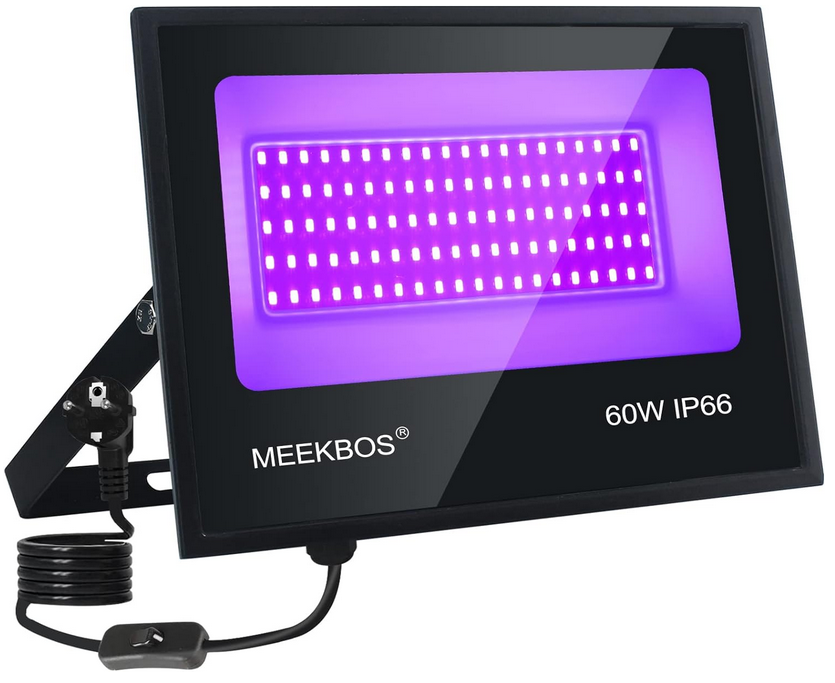
\includegraphics[scale=0.23]{image/uvlampe.png}
\caption{UV-Lampe\autocite{https://m.media-amazon.com/images/I/617AufdHaoL._AC_SL1500_.jpg}}
\end{figure}
\newpage
Die UV-Lampe wird nicht direkt vom \raspi gesteuert. Zwischen dem \raspi und der Lampe ist ein Relais. Dies ermöglicht es, mit einer Spannung von 5V vom \raspi die 230V Netzspannung zu schalten.\\
\vspace{3mm}
\begin{table}[H]
    \centering
    \begin{tabular}{ | c | c | } 
  \hline
   VDD & 5 Volt\\ 
  \hline
   GND & Ground\\ 
  \hline
   Datenleitung (NC) & GPIO18\\ 
  \hline
   Signal (SIG) & GPIO23\\ 
  \hline
\end{tabular}
    \caption{Pinbelegung UV-Lampe}
\end{table}
\vspace{1mm}
Die Programmierung für das Testprogramm befindet sich im Kapitel \ref{sec:Testprogramm UV-Lampe}, und der Programm Abschnitt für die API im Kapitel \ref{sec:Einschalten}

\newpage
\subsection{Magnetfeld}\label{sec:Magnetfeld}
Der CubeSat befindet sich später in einer Umlaufbahn der Magnetosphäre, deshalb soll der CubeSat in der Testkammer einem Magnetfeld ausgesetzt werden.\\
\vspace{5mm}
Die Magnetosphäre ist eine Region die die Erde umschließt, um die Oberfläche von Sonnenwinden zu schützen. Diese Region besitzt ein Magnetfeld. Das Magnetfeld der Magnetosphäre wird durch den Erdkern erzeugt. Die Grenze für die Magnetosphäre ist unbekannt, da diese Region weit ins Weltall reicht.\\
\vspace{5mm}
Es wurden Neodym Dauermagnete\autocite{Magnet} eingesetzt, um das Magnetfeld zu erzeugen.\\
\vspace{3mm}
Ein Neodym Magnete erzeugt ein Magnetfeld im Bereich von einigen Hundert bis mehreren Tausend Gauss. Das Magnetfeld der Erde ist sehr schwach. Es besitzt eine größe von 0,7 Gauss.\\
\vspace{3mm}
Diese Magnete werden in der Kammer befestigt. Die ursprüngliche Idee war, die Magnete am Gyroskop zu befestigen. Da diese Magneten jedoch ein sehr starkes Magnetfeld erzeugen, werden sie weiter weg platzier.\\
\vspace{5mm}
\begin{figure}[H]
    \centering
    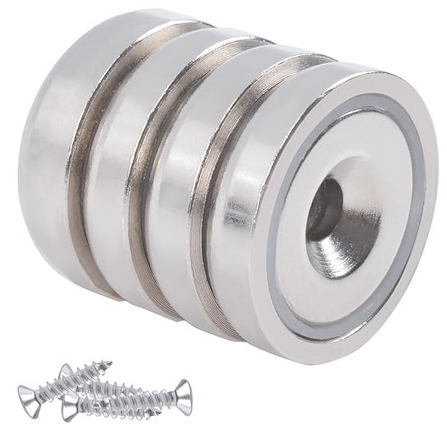
\includegraphics[scale=0.4]{image/Magnet.png}
    \caption{Dauermagnet\autocite{Beispielbild_Magnet}}
    \label{fig:enter-label}
\end{figure}


\newpage
\SecAuth{\nameJS}
\subsection{Pneumatik}\label{sec:Pneumatik}
Um ein Vakuum zu erzeugen und um den Satelliten rütteln zu lassen, werden Pneumatik Teile benötig.
Pneumatik ist ein Bereich der Technik, der Druckluft nutzt, um mechanische Arbeit einfach zu verrichten. Es bietet eine vielseitige und sichere Methode für verschiedene Anwendungen wie Automatisierung, Maschinenbau und Fahrzeugtechnik. Durch die Verwendung von pneumatischen Aktuatoren wie Zylindern und Ventilen können Bewegungen gesteuert und automatisiert werden. Insgesamt ermöglicht Pneumatik eine effiziente und zuverlässige mechanische Leistung. Für die Teststation werden folgende Pneumatik Teile benötigt:
\vspace{3mm}
\begin{table}[H]
    \centering
    \begin{tabular}{ | c | c | } 
  \hline
   \textbf{Bezeichnung} & \textbf{Stückzahl}\\ 
  \hline
   Ventil 24 VDC & 1\\ 
  \hline
    Ventil 24 VDC, Druck justierbar & 1 \\ 
  \hline
  Vakuum Ejektor & 1 \\ 
  \hline
  Druckluft Kugel Vibrator & 1 \\ 
  \hline
\end{tabular}
    \caption{Stückliste Pneumatik}
\end{table}
\vspace{2mm}
Mit den beiden Ventil können wir die Luftzufuhr zu dem Vakuum Ejektor und dem Druckluft Kugel Vibrator steuern. Mit dem Vibrator können wir eine Rüttelplatte verwirklichen und können so den Satelliten auf Vibrationen testen. Die Pneumatik Teile wurden uns von der Firma Hefel Technik GmbH gesponsert, die spezialisiert auf Pneumatik und Automatisierungstechnik sind.\\
\newpage
\textbf{Komplette Zusammenschaltung Pneumatik}\\
\vspace{3mm}
\begin{figure}[H]
    \centering
    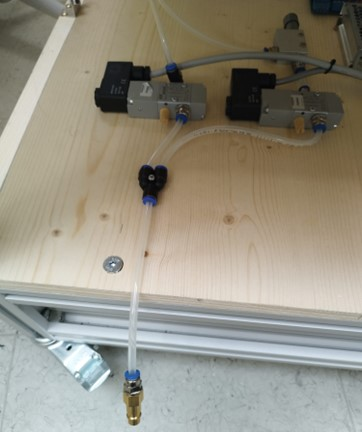
\includegraphics[scale=0.6]{image/zusammenpneumatik.jpg}
    \caption{Zusammenschaltung Pneumatik}
    \label{fig:enter-label}
\end{figure}


\subsubsection{Ventil}
Das VY-83ELB00-T\autocite{Ventil} ist ein pneumatisches Ventil, das häufig in der Industrie eingesetzt wird, um den Durchfluss von Druckluft zu steuern. Mit diesem Ventil steuern wir die Rüttelplatte und den Vakuum Ejektor. So ein Ventil besteht aus einem elektromagnetischen Spulenmechanismus, der einen beweglichen Ventilspulenkern betätigt, um den Luftstrom zu öffnen oder zu schließen. Das VY-Solenoidventil bietet eine zuverlässige und präzise Steuerung des Luftstroms, was es ideal für Anwendungen in der Automatisierung, Maschinenbau und anderen industriellen Bereichen macht.\\
\vspace{3mm}
\begin{figure}[H]
    \centering
    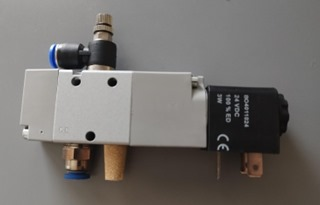
\includegraphics{image/ventil.jpeg}
    \caption{Ventil}
    \label{fig:enter-label}
\end{figure}
\vspace{3mm}
Steuern kann man das Ventil, in dem man eine Spannung anschließt. Werden 24V eingespeist, öffnet das Ventil und die Luft kann durchströmen. Sobald die Spannung entzogen wird, schließt sich das Ventil wieder. Die Spannungszufuhr wird mit einem Relais gesteuert.
\begin{figure}[H]
    \centering
    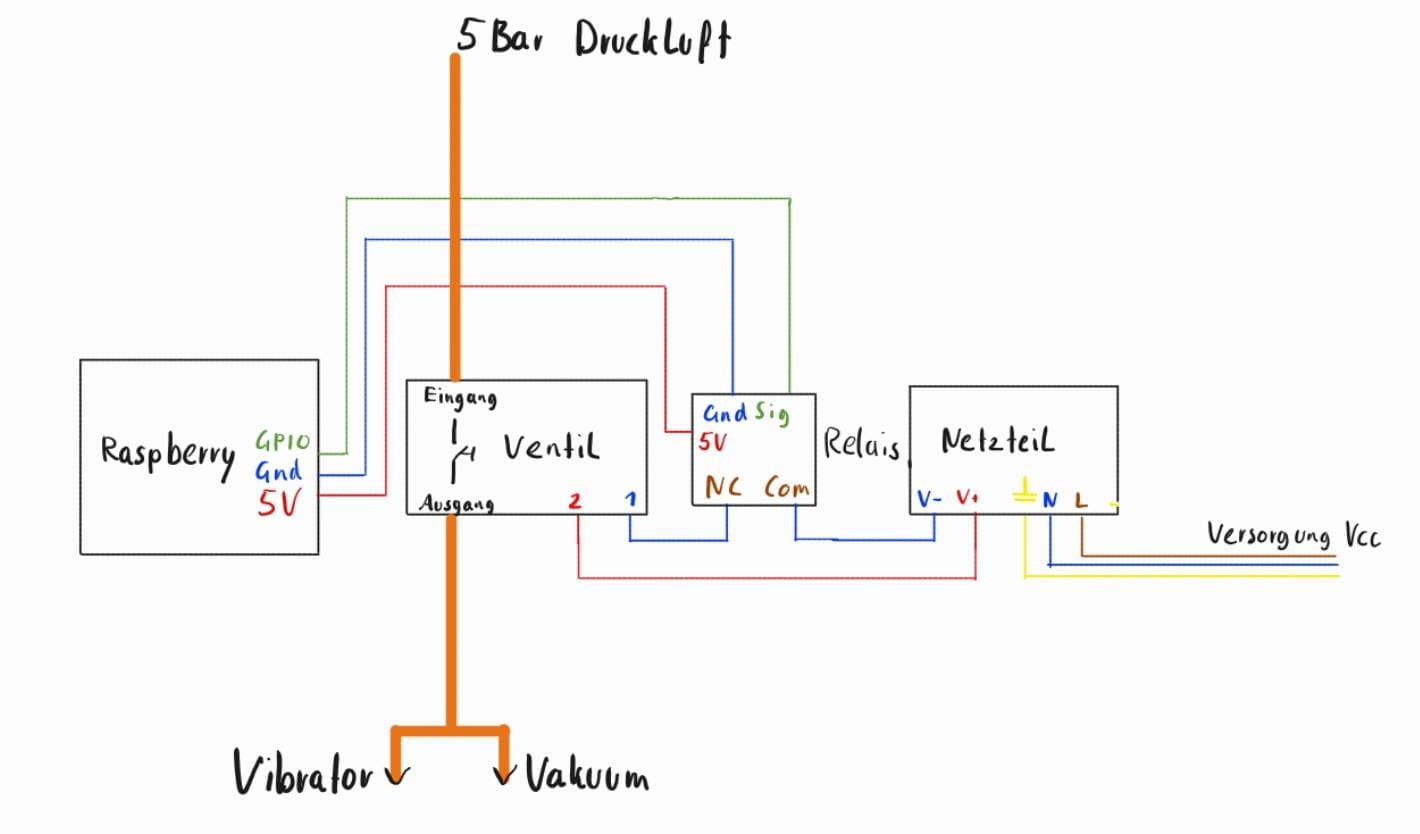
\includegraphics[scale=0.3]{image/zusammenschaltngventil.jpeg}
    \caption{Zusammenschaltung Ventil}
    \label{fig:enter-label}
\end{figure}

\subsubsection{Vakuum Ejektor}
Da wir den Satelliten in einem Vakuum testen müssen, benötigen wir ein Vakuum Erzeuger. Ein Vakuum ist ein physikalischer Zustand, der durch das Fehlen von Materie in einem bestimmten Bereich gekennzeichnet ist. Es ist ein Raum, der frei von Gasen, Flüssigkeiten oder Feststoffen ist. In einem Vakuum gibt es keinen atmosphärischen Druck, da kein Medium vorhanden ist, das diesen Druck ausüben könnte. Da der Weltraum nahezu leer von Materien ist und deshalb ein Vakuum ist, wird der Satellit auch auf diese Einflüsse getestet.\\
\vspace{3mm}
Ein Vakuum-Ejektor\autocite{VakuumEjektor} erzeugt ein Vakuum durch Absaugen von Luft oder Gas aus einem geschlossenen Raum. Dies geschieht durch Hochdruckluft, die durch eine Düse strömt und einen Unterdruck erzeugt. Vakuum-Ejektoren sind effizient, zuverlässig und erfordern wenig Wartung. Mit dem Ventil kann der Vakuum Ejektor gesteuert werden.\\
\newpage
Wir haben uns für den Typ CV\autocite{VakuumEjektor} entschieden, da dieser haltbar und langlebig und langlebig ist, dieser Typ ist der beliebteste Ejektor.
Mit diesem kann ein Vakuumwert von - 0,58 oder  - 0,92 Bar erreicht werden.
\vspace{3mm}
\begin{figure}[H]
    \centering
    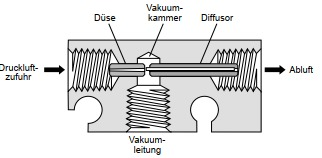
\includegraphics[scale=1.2]{image/vakuumejektor.jpeg}
    \caption{Skizze Vakuum-Ejektoren\autocite{VakuumEjektor}}
    \label{fig:enter-label}
\end{figure}
\vspace{3mm}
Der Satellit wird dann in eine Vakuum Glocke gegeben. Eine Vakuumglocke ist eine abgedichtete Glaskuppel, die in unserem Fall über den Satelliten platziert wird, um ein Vakuum zu erzeugen. Sie schützt den Satelliten vor äußeren Einflüssen wie Luft, Staub oder Feuchtigkeit und wird oft in Labors und Werkstätten verwendet, um eine kontrollierte Atmosphäre zu schaffen.


\subsubsection{Druckluft Kugel Vibrator}
Ein pneumatischer Kugelvibrator ist ein Gerät, die verwendet wird, um Vibrationen zu erzeugen, indem Druckluft durch einen Hohlraum geleitet wird, der eine Kugel enthält. Hier ist eine Beschreibung, wie ein pneumatischer Kugelvibrator funktioniert:
Ein pneumatischer Kugelvibrator besteht aus einem Gehäuse, das eine oder mehrere Kugeln enthält, die sich frei bewegen können. Das Gehäuse hat Ein- und Auslassöffnungen, durch die Druckluft ein- und austreten kann. Die Zufuhr wird mit einem Ventil gesteuert.\\
Druckluft wird durch die Einlassöffnung in das Gehäuse geleitet, der Druck wird mit dem Ventil gesteuert. Diese Luftströmung erzeugt eine Druckdifferenz im Inneren des Gehäuses, die die Kugel oder Masse dazu bringt, sich zu bewegen.\\
\vspace{3mm}
Wenn die Druckluft in das Gehäuse strömt, dreht sich die Kugel im Inneren. Diese Bewegung erzeugt Vibrationen, die auf das umgebende Material oder die Maschine übertragen werden.\\
\vspace{3mm}
Die Intensität der Vibration kann durch die Steuerung des Luftdrucks und der Luftströmung gesteuert werden. Durch Anpassen dieser Parameter kann die Vibrationsstärke des Kugelvibrators angepasst werden.\\
\vspace{3mm}
\begin{figure}[H]
    \centering
    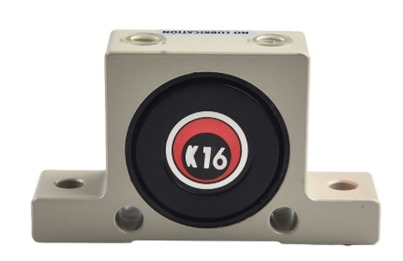
\includegraphics{image/vibration.jpeg}
    \caption{Druckluft Kugel Vibrator\autocite{PneumatischerVibrator}}
    \label{fig:enter-label}
\end{figure}
\subsubsection{Rüttelplatte}
Um den Druckluft Kugel Vibrator zu verwenden, muss eine Plattform gebaut werden, die beweglich ist, aber trotzdem fix verschraub bar ist.  Dazu sind sogenannt Schwingungsdämpfer nötig. Diese bestehen aus  Gummi und können mit M8 Schrauben befestigt werden. Auf die Plattform wird der Satellit platziert und kann durchgeschüttelt werden.
Die Rüttelplatte wird an den Dämpfungselementen mit einem Rest-Aluprofile verschraubt. \\
\vspace{3mm}
\begin{figure}[H]
    \centering
    \begin{subfigure}[b]{0.4\textwidth}
        \centering
        \includegraphics[width=\textwidth]{image/rüttelplatte1.jpeg}
        
        \label{fig:bild1}
    \end{subfigure}
    \hfill
    \begin{subfigure}[b]{0.47\textwidth}
        \centering
        \includegraphics[width=\textwidth]{image/rüttelplatte2.jpeg}
        
        \label{fig:bild2}
    \end{subfigure}
    \caption{Rüttelplatte}
    \label{fig:zwei_bilder}
\end{figure}
\vspace{3mm}
Da die Schrauben von den Schwingungsdämpfern zu kurz sind, werden sie an einer Aluplatte befestigt. Diese Platte ist mit dem Vibrator verschraubt. Eine zweite Aluplatte ist notwendig, um den Satelliten drauf zu stellen. Die Schrauben werden mit Schraubkleber beschmiert, da sie sich sonst bei ständigen Vibrationen lösen.
\newpage
\subsection{LED-Streifen}\label{sec:LED}
Da die PVC-Platten sehr dunkel sind und nur durch die Tür Licht in die Kammer kommt, ist eine Beleuchtung notwendig. Dies wird mit einem einfachen LED-Streifen umgesetzt. Der gewählte LED-Streifen wird mit 24V versorgt und kann dank dem IC WS2811 mit dem Raspberry gesteuert werden. Es kann ein warmes oder kaltes Licht erzeugt werden. \\
\vspace{3mm}
Schaltplan:\\
\vspace{2mm}
\begin{figure}[H]
    \centering
    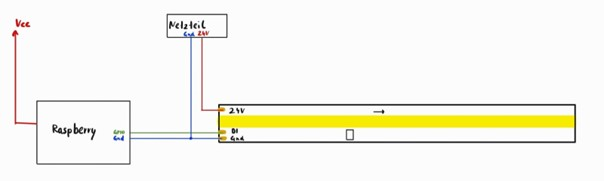
\includegraphics[scale=1]{image/schaltplanled.jpg}
    \caption{Schaltplan LED}
    \label{fig:enter-label}
\end{figure}
\vspace{3mm}
Der LED-Streifen wird mit demselben Netzteil als der Motor versorgt. Dieses liefert genau 24V. DI auf dem LED-Streifen steht für Daten In und wird über einen GPIO-Pin gesteuert. GND geht jeweils zum Raspberry Pi und zum Netzteil. \\
\vspace{3mm}
Damit auch die Ecken sauber an den Deckel der Kammer geklebt werden kann, wurde der LED-Streifen auseinandergeschnitten, um 90° gedreht und wieder mit Kabel verbunden. Da der UV-Strahler an dem Decker auf einem Aluprofil montiert ist, muss das Kabel über das Profil gehen, um eine durchgängige Verbindung zu erhalten. \\
\vspace{3mm}
Bei der Verdrahtung ist zu beachten, dass die Pfeile auf dem Streifen berücksichtig werden. \\
\vspace{3mm}
\begin{figure}[H]
    \centering
    \begin{subfigure}[b]{0.52\textwidth}
        \centering
        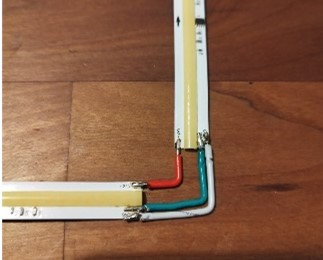
\includegraphics[width=\textwidth]{image/led1.jpg}
        
        \label{fig:bild1}
    \end{subfigure}
    \hfill
    \begin{subfigure}[b]{0.45\textwidth}
        \centering
        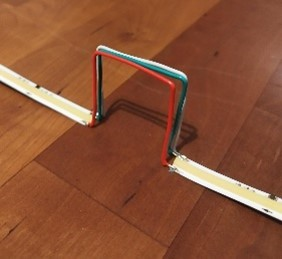
\includegraphics[width=\textwidth]{image/led2.jpg}
       
        \label{fig:bild2}
    \end{subfigure}
    \caption{LED Verbindung}
    \label{fig:zwei_bilder}
\end{figure}
 
\newpage
\SecAuth{\nameSB}
\subsection{CubeSat}\label{sec: CubeSat}

Der CubeSat, initiiert vom TU Wien Space Team, ist eine Bildungsmission, die im August 2020 gestartet wurde. Es handelt sich um einen CubeSat, der entwickelt wurde, um Schülern in Österreich die Möglichkeit zu bieten, eigene Software auf ihm auszuführen. Der Satellit enthält eine Bildungsnutzlast mit einem Raspberry Pi, Sensoren und Kameras, die von Schülern über Python programmiert werden können. Ziel ist es, durch den Betrieb dieses CubeSats und einer eigenen Bodenstation das Interesse und Wissen über Raumfahrttechnologien zu fördern.\\
\begin{figwindow}[0,r,\includegraphics[scale=0.7]{image/3dcube.png},{3D-Modell des CubeSats}]
Das detaillierte Modell des CubeSats im Dateiformat für SolidWorks habe ich von der Technischen Universität Wien erhalten. Dieses hochpräzise Modell stellt eine wesentliche Ressource für die Diplomarbeit dar. Das bereitgestellte CubeSat-Modell zeichnet sich durch seine Detailgenauigkeit aus. 
\end{figwindow}
\vspace{25mm}
\begin{figure}[H]
    \centering
    \includegraphics[scale = 0.8]{image/Druckvorbereitung.png}
    \caption{Druckvorbereitung von zwei Teilen des CubeSats}
    \label{fig:enter-label}
\end{figure}
\newpage
Wie man dem Bild entnehmen kann, sieht man auch, wie lange der Druckvorgang dauert, wie viele Meter Filament benötigt werden und wie viel der Druck wiegt.\\ 
Da sechs Seiten mit dem 3D-Drucker gedruckt werden müssen und maximal zwei Teile gleichzeitig gedruckt werden können, muss man den Vorgang mit den jeweiligen Teilen noch zweimal wiederholen. \\
\vspace{3mm}
\begin{figwindow}[0,r,\includegraphics[scale=0.7]{image/ausdruck.png},{Ausgedrucktes Modell des CubeSats}]
Nachdem alle Teile des CubeSats gedruckt worden sind, muss der CubeSat noch zusammengeschraubt werden.  
\end{figwindow}
\vspace{55mm}
Um den Raspberry Pi sicher an einer Metallplatte zu befestigen, wurden vier Löcher in die Platte gebohrt. Für die Montage kamen spezielle Kunststoffschrauben, Standbolzen und Muttern zum Einsatz, um Kurzschlüsse zu vermeiden.\\
\vspace{3mm}
\begin{figure}[H]
    \centering
    \includegraphics[scale = 0.7]{image/metalplatte.jpg}
    \caption{Raspberry Pi an der Metallplatte befestigt}
    \label{fig:enter-label}
\end{figure}
Der Raspberry PI wurde aufgrund von Stabilitätsgründen mit Abstandbolzen auf einer Metallplatte montiert und aus Isolationsgründen wurden Abstandsbolzen aus Kunststoff verwendet. Durch diese sorgfältige Vorgehensweise konnte ich sicherstellen, dass der Raspberry Pi optimal für seinen Einsatz im CubeSat vorbereitet ist, ohne die Sicherheit und Zuverlässigkeit des Systems zu gefährden.\\
\vspace{3mm}
\begin{table}[H]
    \centering
    \begin{tabular}{ | c | c | } 
  \hline
   \textbf{Bezeichnung} & \textbf{Stückzahl}\\ 
  \hline
   Kunststoffschrauben (M2,5) & 4\\ 
  \hline
  Kunststoffstandbolzen & 4 \\ 
  \hline
  Kunststoffmuttern & 4\\
  \hline
\end{tabular}
    \caption{Stückliste CubeSat}
\end{table}
Um eine optimale Haftung zu erzielen, wurde die Metallplatte mit dem Epoxidkleber sorgfältig am CubeSat angebracht. Bei diesem Vorgang kommt eine Schraubzwinge zum Einsatz, ein entscheidendes Werkzeug, um Druck auszuüben und so die Platte während des Aushärteprozesses des Klebers fest an ihrem Platz zu halten.\\
\vspace{3mm}
Die Schraubzwinge gewährleistet, dass der Kleber gleichmäßig verteilt wird und keine Luftblasen oder Unregelmäßigkeiten die Verbindung schwächen können. Diese Methode garantiert eine hohe Zuverlässigkeit, Stabilität und Halt für die späteren Rotationstests.\\
\vspace{3mm}
\begin{figure}[H]
    \centering
    \includegraphics[scale = 0.7]{image/fertigercube.jpg}
    \caption{Fertiges CubeSat-Modell}
    \label{fig:enter-label}
\end{figure}
Abbildung zeigt den CubeSat mit der erfolgreich angepassten Aluminiumplatte mit dem Raspberry Pi.\\

\newpage
\subsection{Halterung}\label{sec: Halterung}
Das Konzept für die Halterung des CubeSats zielt darauf ab, eine effektive Lösung zu finden, um den CubeSat am Gyroskop zu befestigen. Dabei gilt es zu beachten, dass möglichst alle Seiten des CubeSats offen und zugänglich bleiben. Die Halterung soll an zwei Punkten mit dem Gyroskop befestigt werden. \\
\vspace{3mm}
Der Kern dieses Konzepts ist ein Käfigsystem, das aus zwei Hauptteilen besteht, nämlich einem Boden und einem Deckel. Dieses Design ist speziell darauf ausgelegt, den CubeSat vollständig zu umschließen und durch Schrauben sicher zu fixieren. Es gibt dann somit am Boden und am Deckel jeweils einen Verbindungspunkt zum Gyroskop.\\
\subsubsection{Boden}
\begin{figure}[H]
    \centering
    \includegraphics[scale = 0.5]{image/boden.jpg}
    \caption{Boden}
    \label{fig:enter-label}
\end{figure}
\vspace{3mm}
Das Bild zeigt eine technische Zeichnung einer rechteckigen Grundfläche mit den Maßen 130 mm in der Länge, 115 mm in der Breite und einer Materialstärke von 8 mm. Vier Pfosten erstrecken sich von den Ecken der Grundfläche, wobei die Pfostenlänge 77 mm beträgt.\\
\vspace{3mm}
In jedem Pfosten befindet sich eine Gewindebohrung, die eine Tiefe von 15 mm aufweist und für Schrauben mit einem Durchmesser von 4 mm vorgesehen ist. Im Mittelpunkt der Grundfläche ist ein Loch eingezeichnet, das als Befestigungspunkt für ein Gyroskop dient.\\
\vspace{3mm}
\begin{figure}[H]
    \centering
    \includegraphics[scale=0.7]{image/zusätzlichehalterung.jpg}
    \caption{Zusätzliche Halterung }
    \label{fig:enter-label}
\end{figure}
\vspace{3mm}
Jede Ecke der Struktur wird verstärkt, indem an jeder Ecke zwei zusätzliche Stützen angebracht werden. Diese Stützen dienen dazu, den CubeSat sicher und fest in der Struktur zu verankern, indem sie zusätzlichen Halt bieten und verhindern, dass sich der Satellit innerhalb des Trägerrahmens bewegt.\\
 \begin{figure}
     \centering
     \includegraphics[scale=0.5]{image/fertiger boden.jpg}
     \caption{fertiger Boden}
     \label{fig:enter-label}
 \end{figure}

Um einen noch besseren Halt des CubeSats sicherzustellen, habe ich weitere Stützen jeweils in der Mitte der Grundfläche angebracht. Diese spannen den CubeSat noch besser ein und bieten dadurch eine noch bessere Stabilität.\\

\subsubsection{Deckel}
\begin{figure}[H]
    \centering
    \includegraphics[scale=0.7]{image/deckel.png}
    \caption{Deckel}
    \label{fig:enter-label}
\end{figure}
\vspace{3mm}
Das Bild zeigt die technische Zeichnung einer rechteckigen Grundfläche, welche in seinen Grundmaßen und Konstruktionsmerkmalen dem Bodenteil ähnelt.\\
\vspace{3mm}
Die Abmessungen des Rechtecks betragen 130 mm in der Länge und 115 mm in der Breite, mit einer Toleranz von ±0,50 mm, und die Materialdicke ist ebenfalls gleichbleibend. Auch der Deckel hat im Mittelpunkt ein Loch, welches als Verbindung zum Gyroskop dient.\\
\vspace{3mm}
Der wesentliche Unterschied zwischen dem Deckel und dem Boden des Geräts besteht in der Länge der Pfosten, die beim Deckel auf 23 mm reduziert wurde, um eine Verbindung mit dem Boden mittels 4 cm langen Schrauben zu ermöglichen. Diese Anpassung sorgt für eine sichere Befestigung zwischen beiden Teilen.\\
\vspace{3mm}
Ein weiteres wichtiges Detail ist die Art der Löcher in den Pfosten. Während die Pfosten des Bodens Gewindebohrungen mit einer Tiefe von 15 mm aufweisen, die für Schraubverbindungen vorgesehen sind, sind die Pfosten des Deckels mit durchgehenden Löchern versehen. \\ 
\vspace{3mm}
Diese durchgehenden Löcher erlauben es, Befestigungselemente komplett durch die Pfosten hindurchzuführen, was eine durchgängige Verbindung zwischen dem Deckel und dem Boden aufweist.
\newpage
\subsubsection{3D-Druck der Halterung}
Um den Boden und den Deckel drucken zu können, müssen die STL-Dateien in Dremel DigiLab 3D Slicer wie folgt verarbeitet werden:\\
\vspace{3mm}
Als erstes wird das 3D-Modell (üblicherweise im. stl-Format) importiert. Danach wird das Modell auf der virtuellen Druckplatte platziert und nach Bedarf angepasst. Anschließend wird das Material ausgewählt und die Druckqualität sowie die Füllungsdichte festgelegt. \\
\vspace{3mm}
Bei Bedarf können auch Stützstrukturen hinzugefügt werden und Raft und Brim für eine bessere Haftung auf der Druckplatte genutzt werden. Mit Klicken auf „Slice“ wird eine Gcode-Datei erzeugt, welche dann auf den 3D-Drucker übertragen und gedruckt werden kann.
\vspace{3mm}
\begin{figure}[H]
    \centering
    \includegraphics[scale=0.7]{image/druckvorbereitungboden.png}
    \caption{Druckvorbereitung für den Boden}
    \label{fig:enter-label}
\end{figure}
\vspace{3mm}
Abbildung zeigt, wie lange der Druckvorgang geht, wie viele Meter Filament benötigt wird und wie viel der Druck wiegt. Dieser Vorgang muss für den Deckel wiederholt werden.\\
\vspace{3mm}
\begin{figure}[H]
    \centering
    \includegraphics[scale=0.7]{image/cubeinhalterung.jpg}
    \caption{CubeSat in der Halterung}
    \label{fig:enter-label}
\end{figure}
\vspace{3mm}
Der CubeSat ist sicher im Käfig verankert. Der Käfig selbst besteht aus einer Struktur, die mit Schrauben und Muttern an den Ecken zusammengehalten wird. Die Konstruktion ist stabil und robust, was für eine gute Haltbarkeit spricht und somit bestens für die Rotationstests im Gyroskop geeignet ist. \\
\vspace{3mm}
\begin{table}[H]
    \centering
    \begin{tabular}{ | c | c | } 
  \hline
   \textbf{Bezeichnung} & \textbf{Stückzahl}\\ 
  \hline
   Schrauben  & 4\\ 
  \hline
  Muttern & 4 \\ 
  \hline
\end{tabular}
    \caption{Stückliste Halterung}
\end{table}
\input{Lüftung}
\newpage
\input{Kühlung}
\newpage
\SecAuth{\nameJS}
\subsection{Sicherheit}\label{sec:sicherheit}

\subsubsection{Notausschalter}
Ein Notausschalter sogt dafür, dass das Gyroskop im Notfall sofort ausgeschalten werden kann. Um den Notaus zu implementieren gib es 2 verschiedene Möglichkeiten, eine Softwarelösung und eine Hardwarelösung. Beide Möglichkeiten haben ihre Vor- und Nachtteile und diese werden genauer beschrieben.\\
\vspace{3mm}
Bei der Hardwarelösung wird durch Betätigen des Schalters die Spannungsversorgung vom Netzteil unterbrochen und der Motor stoppt. Die Implementation wäre sehr einfach, doch bei der Hardwarelösung  ist das Problem, wenn der Notaus wieder entriegelt wird, der Motor sofort wieder zu drehen beginnt.\\
\vspace{3mm}
Bei der Softwarelösung wird der Notausschalter mit dem Raspberry Pi verbunden und bei Betätigen des Tasters erkennt der Raspberry ein Low Input an einem GPIO-Pin und schaltet der Motor aus. Diese Version ist aber nicht zuverlässig genug, denn wenn der Raspberry eine Störung hat oder das Input Signal nicht erkannt wird, dreht sich das Gyroskop weiter und stellt somit eine Gefahr für den Satelliten dar. Der Vorteil dieser Variante ist, dass programmiert werden kann, dass der Motor nach Entriegelung des Notaus nicht automatisch wieder gestartet wird.\\
\vspace{3mm}
Da beide Lösungen wichtige Funktionen haben, werden die beiden Variante miteinander verbunden. Der Notausschalter wird zwischen die Spannungsversorgung verbunden und mit einem Relais, das an den Raspberry Pi geschlossen wird, wird der Zustand geprüft. Wird der Notausschalter gedrückt, muss mit einem Software Button das Relais wieder geöffnet werden. Durch diese Implementierung wird ein automatisches Starten nach Entriegelung des Notausschalter verhindert. Dies nennt man quittieren, was so viel bedeutet wie bestätigen. Damit man im User Interface um quittieren erinnert wird, blinkt der Quittierungsbutton ROT. 
\pagebreak
\subsubsection{Schlüsselschalter}
Damit nicht jeder die Berechtigung hat, die Teststation in Betrieb zu nehme, wird ein Schlüsselschalter eingebaut. Wird mit dem Schlüssel der Schalter gedreht, hat man den vollen Zugriff auf die Steuerung mit dem Raspberry Pi. \\
\vspace{3mm}
\begin{figure}[H]
    \centering
    \includegraphics[scale=0.8]{image/schlüsselschalter.jpg}
    \caption{Schlüsselschalter}
    \label{fig:enter-label}
\end{figure}
\subsubsection{Endschalter}
Endschalter sind Schalter, die Endposition eines mechanischen Systems erfassen. Sie kommen in verschiedenen Anwendungen wie Maschinenbau, Automatisierungstechnik und Robotik zum Einsatz, um das Erreichen eines bestimmten Punktes zu erkennen. Ihre Verwendung trägt zur Sicherheit und Effizienz von Maschinen und Systemen bei, indem sie das Erreichen der Endpunkte von Bewegungen oder Prozessen signalisieren.\\
\vspace{3mm}
Verkabelung und Befestigung:
Im Rahmen gibt es zwei kleine Aussparungen, in denen die Endschalter platziert werden. Wird nun die Tür geschlossen, werden die Schalter betätigt.\\
\vspace{5mm}
\begin{figure}[H]
    \centering
    \includegraphics{image/Zusammenschaltung-Endschalter.png}
    \caption{Zusammenschaltung Endschalter}
    \label{fig:enter-label}
\end{figure}
Wenn die Teststation während einem Test bewegt wird, könnten durch die Erschütterungen die Endschalter elektrische Störungen erkennen. Um dies zu verhindern, müssen die Endschalter mindestens eine Sekunde lang das jeweilige Signal erkennen. 



\newpage
\section{Software}
\subsection{Tasterabfrage}\label{sec:Tasterabfrage}
\SecAuth{\nameSH}
Die Tasterabfrage wird in verschiedenen Programmabschnitten benötigt. Je nachdem wie oft ein Button gedrückt wird, soll ein anderer Programmteil abarbeitet werden. Dieser Ablauf wird benutzt um zum Beispiel eine Lampe ein und auszuschalten. Um die Tasterabfrage zu realisieren, werden boolsche Variablen verwendet. \\
\vspace{2mm}
Zu beginn des Programm wird eine boolsche Variable festgelegt, diese wird auf \textit{False} gesetzt. Damit die Variable auch im Unterprogramm verwendet werden kann, muss sie zum Beispiel mit \textbf{global} \textit{boolUV} übergeben werden. In der nächsten Zeile wird der Zustand der Variable gewechselt. Da diese am Anfang auf \textit{False} gesetzt ist, wird sie jetzt auf \textit{True} gesetzt. Jedes mal wenn der Button gedrückt wird, durchläuft das Programm diesen Abschnitt. Durch den Wechsel wird dafür gesorgt, dass nach jedem Drücken einer der beiden Codeteile abarbeitet wird. Wenn die boolsche Variable \textit{True} ist, wird der Code der unter dem Abschnitt \textit{True} steht abarbeitet. Das selbe geschieht, wenn die Variable auf \textit{False} gesetzt ist.\\
\vspace{3mm}
\begin{figure}[h]
    \centering
    \begin{minted}{python}
                #globale boolsche Variable
                global boolUV

                #Zustandswechsel
                boolUV = not boolUV

                if boolUV == True :
                    #Code um UV-Lampe einzuschalten
        
                else:
                    #Code um Lampe auszuschalten
    \end{minted}
    \caption{Beispielcode Tasterabfrage}
\end{figure}
\newpage

\subsection{Testprogramm}\label{sec:Testprogramm} 
\SecAuth{\nameJS}
Die Steuerung der Hardware Module wie Motor, Netzteil, UV-Lampe und die Auslesung vom Notaus oder der Sensoren werden mit einer GUI verwirklicht. Diese GUI dient aber nur für Entwicklungszwecke, da diese später von einer API ersetzt wird. Die GUI kann über das LX-Terminal vom Raspberry gestartet werde.
\subsubsection{GUI}\label{sec:GUI}
Um eine GUI zu erstellen und die Ein und Ausgänge vom Raspberry Pi zu steuern, werden 2 Bibliotheken benötigt.\\
\vspace{3mm}
Tkinter: Um eine grafische Benutzeroberfläche zu erstellen, wird die Python-Bibliothek „tkinter“ benötigt. Mit dieser Bibliothek können Fenster, Schaltflächen, Eingabefelder und andere GUI-Elemente erstellt werden.\\
\vspace{3mm}
RPi.GPIO: Die Python Bibliothek RPi.GPIO ermöglicht, mit den Ein und Ausgänge vom Raspberry Pi zu kommunizieren. In unserer Anwendung werden Sensoren eingelesen und externe Geräte gesteuert.\\
\vspace{3mm}
Installieren: Damit man die Bibliotheken verwenden kann, müssen sie auf dem Raspberr Pi installiert werden. Normalerweise ist Tkinter bereits vorinstalliert, doch bei unserem Raspberry Pi nicht. Folgenden Befehlen müssen im Terminal ausgeführt werden um die Bibliotheken zu erhalten.\\
\begin{verbatim}
    Sudo apt-get update
    Sudo apt-get install python3 -tk
    Sudo apt-get install python3-pip
    Sudo pip install Rpi.GPIO
\end{verbatim}
\pagebreak
Einbinde der Bibliotheken:
\begin{figure}[H]
    \centering
    \begin{minted}{python}
    from tkinter import *
    import RPi.GPIO as GPIO
    \end{minted}
    \caption{GUI-Bibliothek einbinden}
\end{figure}
Fenster erstellen: Dieser Code erstellt ein Hauptfenster für eine GUI-Anwendung mit dem Titel "Controll Unit", einem weißen Hintergrund und einem Frame namens rightFrame, das als Container für weitere GUI-Elemente innerhalb des Hauptfensters dient. Die Höhe dieses Fensters ist 800 Pixel und eine Breite von 800 Pixel.\\
\vspace{3mm}
\begin{figure}[H]
    \centering
    \begin{minted}{python}
    #Fenster Erstellen
    root = Tk()
    root.wm_title("Controll Unit")
    root.config(background = "#FFFFFF")
 
    rightFrame = Frame(root, width=500, height =800)
    rightFrame.grid(row=100, column =200, padx=0, pady=3)
    \end{minted}
    \caption{Beispielcode Fenster erstellen}
\end{figure}
Ein weiteres Fenster wird erstellt, um darauf alle Buttons zu platzieren. Dieses ist innerhalb des „rightFrame“ und kann so die GUI zwischen Ein und Ausgabe trennen. Für die Sensordaten wird ein weiteres Fenster erstellt.\\
\vspace{3mm}
\begin{figure}[H]
    \centering
    \begin{minted}{python}
    #GUI-Fenster Erstellen
    buttonFrame = Frame(rightFrame)
    buttonFrame.grid(row=0, column=0, padx=50,pady=3) 
    \end{minted}
    \caption{Beispielcode GUI-Fenster erstellen}
\end{figure}

\newpage
\subsubsection{Button}\label{sec:Button}
Fürs Ein- und Ausschalten von Geräten werden Buttons verwendet. Buttons können in der GUI gedrückt werden und die gewünschte Funktion wird gestartet.\\
\vspace{3mm}
\begin{figure}[H]
	\centering
	\begin{minted}{python}
		#Button erstellen:
		btmot = Button(buttonFrame, text="Exit", bg = "#FF0000",
		width=15,command=exitProgram)
		btmot.grid(row=50, column=1, padx=0,pady=5)
		
		#Button Funktion:
		#Wird der Button gedrückt, wird folgende 
		#Funktion gestartet:
		def btmot():
			#Funktion… 
	\end{minted}
	\caption{Beispielcode Button}
\end{figure}


\subsubsection{Temperatursensor}\label{sec:Testprogramm Temp}
\SecAuth{\nameSH}
Die Temperatursensoren wird nicht über ein Button gesteuert, damit die aktuelle Temperatur immer wieder ausgegeben wird. Die empfangenen Daten werden nach dem Starten des Programms, automatisch auf der GUI angezeigt. Durch die zuvor installierte Bibliothek, werden nur wenige Zeilen an Code benötigt, um Sensordaten auszugeben.
\begin{figure}[H]
    \centering
    \begin{minted}{python}
    #Einbinden der Bibliothek im Programm
    import adafruit_dht
    
    #Definition des Sensors und festlegen des Pins
    dhtDevice1 = adafruit_dht.DHT22(board.D2)     

    #Funktion temperature einer Variable zuweisen
    temp_c = dhtDevice1.temperature                

    #Funktion humidity einer Variable zuweisen                             
    humidity = dhtDevice1.humidity 
    \end{minted}
    \caption{Beispielcode Temperatursensor}
\end{figure}

\newpage
\subsubsection{UV-Sensor}\label{sec:Testprogramm UV-Sensor}
Wie beim Temperatursensor, wird auch hier die Ausgabe direkt nach dem Starten des Programms erfolgen. Es muss die zuvor installierte Bibliothek eingebunden werden. Danach kann auch hier das Programm in wenigen Schritten programmiert werden.
\begin{figure}[H]
    \centering
    \begin{minted}{python}
    #Einbinden der Bibliothek
    import adafruit_ltr390
    
    #I2C-Schnittstelle initialisieren
    i2c = board.I2C()

    #Definition des Sensors und Übergabe des I2C-Schnittstelle
    ltr = adafruit_ltr390.LTR390(i2c)

    while True:
        #Ausgabe der gemessenen Werte
        
        print("UV-Index:", ltr.uvi, 
              "Umgebungslicht in Lux:", ltr.light)
        
    \end{minted}
    \caption{Beispielcode UV-Sensor}
\end{figure}
\newpage
\subsubsection{Drucksensor}\label{sec:Testprogramm Drucksensor}
Der Drucksensor wird im Testprogramm verwendet, um die richtigkeit des Sensors zu überprüfen. Die Werte des Drucksensors können sehr einfach überprüft werden. Indem im Internet nach der Höhe von Rankweil gesucht wird und mit dem gemessenen Wert verglichen werden. 
\begin{figure}[H]
    \centering
    \begin{minted}{python}
    #Einbinden der Bibliothek
    import bmp180
    
    i2c = board.I2C()
        bmp = bmp180.BMP180(i2c)
        bmp.sea_level_pressure = 1013.25
        return{f"Druck: {bmp.pressure:.1f} hPa", 
                f"Meereshöhe: {bmp.altitude:.1f} Meter"}
    \end{minted}
    \caption{Beispielcode Drucksensor}
\end{figure}

\newpage
\subsubsection{UV-Lampe}\label{sec:Testprogramm UV-Lampe}
Damit getestet werden kann, ob und wie gut die Lampe funktioniert, wurde ein Code zur Ansteuerung für das Relais erstellt. Mithilfe des Button und der Tasterabfrage wird die Lampe ein- und ausgeschaltet. 
\begin{figure}[H]
    \centering
    \begin{minted}{python}
    #boolUV als globale Variable deklarieren
    global boolUV
    #wechseln des bool Zustandes
    boolUV = not boolUV

    if boolUV == True :
        #Pin auf High setzten (Lampe wird eingeschalten)
        GPIO.output(PinUV,GPIO.HIGH)
        #Text auf Button ändern
        btuv["text"]= "UV-Lampe aus" 
        #Lampe ein wird ausgegeben
        print("Lampe ein")
        
    else:
        #Pin auf Low setzten (Lampe wird ausgeschalten)
        GPIO.output(PinUV,GPIO.LOW)
        #Text auf Button ändern
        btuv["text"]= "UV-Lampe ein"
        #Lampe aus wird ausgegeben
        print("Lampe aus") 
    \end{minted}
    \caption{Beispielcode UV-Lampe}
\end{figure}

\newpage
\SecAuth{\nameJS}
\subsubsection{Motor}\label{sec:test motor}
Der Motor wird mit einem Button ein und ausgeschalten. Jedes Mal, wenn der Button betätigt wird, sollte der Motor ein oder ausgeschalten werden. Die Buttonabfrage, wurde schon bei der UV-Lampe ausführlich erklärt.  \\
\vspace{3mm}
Da die Masse, die bewegt werden muss, relativ schwer ist, wird der Motor als Rampe programmiert. Der Motor braucht dann ca. 3 Sekunden, bis er die Endgeschwindigkeit erreicht. Mit dieser Programmierung braucht der Motor nicht so viel Kraft, um das Gyroskop in
Bewegung zu bringen und zusätzlich wird eine ruckartige Bewegung verhindert. Beim Ausschalten wird dasselbe Prinzip angewendet, denn sonst würde es die Wicklungen vom Motor negativ in Anspruch nehmen und die Lebensdauer verkürzt.\\
\vspace{3mm}
\begin{figure}[H]
    \centering
    \begin{minted}{python}
    #Initialisierung:
    PUL= 17
    EN=13
    GPIO.setmode(GPIO.BCM)
    GPIO.setup(PUL, GPIO.OUT)
    GPIO.setup(EN, GPIO.OUT)

    #PWM Signal:
    for i in range(10000000):
        GPIO.output(PUL,GPIO.HIGH)
        time.sleep(0.0005)
        GPIO.output(PUL,GPIO.LOW)
        time.sleep(0.0005)

    \end{minted}
    \caption{Beispielcode UV-Lampe}
\end{figure}

\subsubsection{Netzteil}\label{sec:test netzteil}
Das Netzteil kann mit einer Button Betätigung ein und ausgeschalten werden. Dazu wird ein Relais verwendet. Die Funktion des Buttons und der Tasterabfrage \ref{sec:Tasterabfrage} wurde schon erklärt. 
\newpage
\subsubsection{LED-Streifen}\label{sec:test Led}
Um die LED’s zu programmieren wird die Bibliothek „import neopixel“ benötigt. Diese kann in der Console installiert werden.\\
\vspace{3mm}
Mit dieser Bibliothek kann man die LED’s einfach steuern.\\
\vspace{3mm}
Folgender Coder verwirklicht das: Mit der „brightness“ und der „fill“ können die LEDs spezifisch gesteuert werden.\\
\vspace{3mm}
\begin{figure}[H]
	\centering
	\begin{minted}{python}
		global boolLED
		print(boolLED)
		boolLED = not boolLED
		print(boolLED)
		pixels = neopixel.NeoPixel(board.D21, 40, brightness =5)
		pixels.fill((0,0,0))
		if boolLED == True :
		pixels.fill((0,255,0))
		btled["text"]= "LEDs aus"
		print(boolLED)
		else:
		pixels.fill((0,0,0))
		btled["text"]= "LEDs ein"
		print(boolLED)
	\end{minted}
	\caption{Beispielcode LED-Streifen}
\end{figure}


\subsubsection{Schlüsselschalter}\label{sec:test schlüssel}
Hier wird einfach nur geprüft, ob der Schalter auf High oder Low ist.
\begin{figure}[H]
    \centering
    \begin{minted}{python}
    SS=6
    GPIO.setmode(GPIO.BCM)
    GPIO.setup(SS, GPIO.OUT)

    if(GPIO.input(SS) == GPIO.LOW)):
        continue
    else:
    \end{minted}
    \caption{Beispielcode Schlüsselschalter}
\end{figure}

\subsubsection{Notausschalter}\label{sec:test notaus}
Beim Notaus wird derselbe Code wie beim Schlüsselschalter verwendet. Es wird geprüft, ob der Schalter auf High oder Low ist. Die Reaktionszeit, bis das Gyroskop ausgeschalten wird, ist unter 0,5 Sekunden und somit akzeptabel.  
\subsubsection{Endschalter}\label{sec:test end}
Um den Schalterzustand zu erkennen, wird geprüft, ob der Schalter auf High oder Low ist. Sind beide Schalter auf Lauf, ist die Tür geschlossen und der Motor kann gestartet werden. \\
\vspace{3mm}
\begin{figure}[H]
    \centering
    \begin{minted}{python}
    #Initialisierung
    END1= 27
    END2=22
    GPIO.setmode(GPIO.BCM)
    GPIO.setup(END1, GPIO.OUT)
    GPIO.setup(END2, GPIO.OUT)

    #Abfrage
    while(TRUE):
    #Tasterabfrage
    #Motoransteuerung
    if(GPIO.input(END1) == GPIO.LOW) and (GPIO.input(END2) == GPIO.LOW):
        continue
    else:
        break

    \end{minted}
    \caption{Beispielcode Endschalter}
\end{figure}

\SecAuth{\nameSB}
\subsubsection{Kühlung}\label{sec: kühlung test}
Der angepasste Code für den Raspberry Pi dient dazu, den Lüfter eines Kühlgerätes in zwei Stufen zu steuern und gleichzeitig einen Filter zu befeuchten. Dabei wird die Tasterabfrage \ref{sec:Tasterabfrage} genutzt, um zwischen den beiden Zuständen der Kühlung (Ein/Aus) umzuschalten und die Intensität der Kühlung (Stufe 1 oder Stufe 2) sowie die Befeuchtung des Filters zu kontrollieren.\\
\vspace{3mm}
\begin{figure}[H]
    \centering
    \begin{minted}{python}
    #boolUV als globale Variable deklarieren
    global boolKühlung
    #wechseln des bool Zustandes
    boolKühlung = not boolKühlung

    if boolKühlung == True :
        #Pin auf High setzten (Kühlung wird eingeschalten)
        GPIO.output(KuehlungPin, GPIO.HIGH)
        #Text auf Button ändern
        btuv["text"]= "Kühlung Stufe 2" 
        #Filter Pin auf High setzen
        GPIO.output(filterPin, GPIO.HIGH)
        #Ausgabe in der Konsole
        print("Kühlung eingeschalten - Stufe 1")
        
        else:
        #Pin auf Low setzten (Kühlung kurz ausgeschalten)
        GPIO.output(KuehlungPin, GPIO.LOW)
        # Pausiert das Programm kurz für 0.1 Sekunden.
        time.sleep(0.1)
        #Pin auf High setzten (Kühlung wird eingeschalten)
        GPIO.output(KuehlungPin, GPIO.HIGH)
        #Filter Pin auf High setzen
        GPIO.output(filterPin, GPIO.HIGH)
        #Text auf Button ändern
        btuv["text"]= "Kühlung Stufe 1"
        #Ausgabe in der Konsole
        print("Kühlung eingeschalten - Stufe 2")

		#Kühlung Pin und Filter Pin auf Low setzen
		GPIO.output(KuehlungPin, GPIO.LOW)
		GPIO.output(filterPin, GPIO.LOW)
		
		#Ausgabe in der Konsole
		print("Kühlung ausgeschalten")        
    \end{minted}
    \caption{Beispielcode Kühlung}
\end{figure}
\newpage
\subsubsection{Lüfter}\label{sec: lüfter test}
Dieser Code steuert das Ein- und Ausschalten des Lüfters über einen GPIO-Pin des Raspberry Pi, mithilfe der Tasterabfrage \ref{sec:Tasterabfrage}.
\vspace{3mm}
\begin{figure}[H]
    \centering
    \begin{minted}{python}
    #boolUV als globale Variable deklarieren
    global boolLüfter
    #wechseln des bool Zustandes
    boolLüfter = not boolLüfter

    if boolLüfter == True :
        #Pin auf High setzten (Lüfter wird eingeschalten)
       GPIO.output(lueftungPin, GPIO.HIGH)
        #Text auf Button ändern
        btuv["text"]= "Lüfter aus" 
        #Lüfter ein wird ausgegeben
        print("Lüftung eingeschalten")
        
    else:
        #Pin auf Low setzten (Lüfter wird ausgeschalten)
        GPIO.output(lueftungPin, GPIO.LOW)
        #Text auf Button ändern
        btuv["text"]= "Lüfter ein"
        #Lüfter aus wird ausgegeben
        print("Lüftung ausgeschalten")
    \end{minted}
    \caption{Beispielcode Lüfter}
\end{figure}
\newpage
\subsection{Verbindungsmöglichkeit }\label{Verbindung}
\SecAuth{\nameCZ}
In Bezug auf die Teststation sollen alle Daten der Sensorik extern über ein drahtloses Verfahren auf einem Laptop/PC empfangen werden, da eine serielle Verbindung durch das Gyroskop in der Teststation viele Komplikationen mit sich bringt. Die Möglichkeiten für solch einen drahtlosen Empfang sind TCP, UDP oder Bluetooth. \\
\vspace{3mm}
Da der CM3+ im Cubesat kein WLAN/Bluetooth-Modul aufweist, muss ein externes Modul über die USB2.0 Schnittstelle am Raspberry PI angeschlossen werden. Ein sogenannter „Dongle“ (USB/Wifi-Bluetooth Modul) wird hierbei verwendet. Da keine normale USB-Buchse am CM3+ angebracht ist (siehe Abb. 90), muss der Dongle mit dem CM3+ durch eine andere Möglichkeit verbunden werden. Das Erstellen einer Buchse für die Verbindung des Dongles wäre hier von Vorteil. \\
\vspace{3mm}
\begin{figure}[H]
	\centering
	\includegraphics[scale=0.8]{image/cm3+.png}
	\caption{Bild des CM3+ von Raspberry PI}
\end{figure}
\vspace{3mm}
\subsubsection{UDP}\label{udp}
Da für die Simulation des Cubesats ein Raspberry PI 4 benutzt wurde, konnte zuerst das WIFI-Modul auf dem Einplatinencomputer verwendet werden. Für die Kommunikationsmethode wurde dafür das UDP-Protokoll genutzt, welches eine schnelle Datenübertragung sicherstellt. UDP\autocite{UDP} dient als minimales Netzwerkprotokoll, das sich für das Versenden von Datenpaketen über das Internet eignet. UDP verwendet keine Handshakes, um eine Verbindung zwischen zwei Endgeräten herzustellen. Dies bedeutet, dass Daten ohne vorherige Kommunikation gesendet werden. Das Protokoll führt zu einer schnelleren Übertragung als TCP, ist jedoch beim Datentransfer unzuverlässiger.

\subsubsection{TCP}
TCP\autocite{TCP} (transmission control protocol) bietet auch eine gute Übertragungsmöglichkeit, da es mit der Hilfe von dem „Handshake-Vereinbarung“ (siehe Abb. 91) eine fehlerfreie Übertragung des Pakets garantiert. Durch die längere Sendezeit des TCP-Protokolls eignet sich das Protokoll für eine zeitkritische Aufnahme von Daten, wie bei der Teststation vorhanden, nicht.\\
\vspace{3mm}
\begin{figure}[H]
	\centering
	\includegraphics[scale=1.1]{image/sendeverfahren.png}
	\caption{Sendeverfahren des TCP-Protokolls\autocite{TCP-Handshake}}
\end{figure}
\vspace{3mm}
Bei dem „Dreifach Handshake Verfahren“, werden SYN- und ACK-Pakete zwischen zwei Endgeräten ausgetauscht. Der Austausch beginnt mit einem SYN-Paket des Clients, gefolgt von einem SYN-ACK-Paket des Servers. Anschließend wird noch ein ACK-Paket vom Client zum Server geschickt. Durch diese Reihenfolge wird sichergestellt, dass Datenpakete in der richtigen Reihenfolge und ohne Fehler übertragen werden. Auch ermöglicht das Protokoll eine Flusskontrolle, um möglichen Datenstau zu vermeiden.

\subsubsection{Serielle Verbindungsmöglichkeit}
Beginn wurde eine Verbindung über die Schnittstelle UART probiert. Hierbei wird der Raspberry PI über die RX und TX-Pins mit einem Serial/USB Adapter mit einem PC verbunden.\\
\vspace{3mm} 
Damit solch eine Verbindung funktioniert müssen die Jumper-Kabel so angeschlossen werden, dass der RX-Pin des Senders mit dem TX-Pin des Empfängers und der TX-Pin des Senders mit dem RX-Pin des Empfängers verbunden ist.\\
\vspace{3mm}
Anschließend lässt sich über die PySerial Bibliothek eine serielle Verbindung erstellen. Für die Datenaufnahme am PC können verschiedene Programme wie TerraTerm oder RealTerm verwendet werden. Auch kann ein eigenes Programm geschrieben werden, welches den Prozess kontrollierbarer macht. \\
\vspace{3mm}
Für die Testung der Verbindung wurde ein kleines Programm auf dem Raspberry PI entwickelt, welches Daten über die serielle Schnittstelle sendet und vom Computer über TerraTerm empfangen wird. Für solch ein Skript muss zuerst der serielle Port des Raspberry Pis geöffnet werden. Dies kann über das Interface Menu in der Raspberry PI Config unter „sudo raspi-config“ eingestellt werden. Der Name des Ports und alle anderen offenen Ports lassen sich unter „/dev  \$ ls“ anzeigen. 
\vspace{3mm}
Nun kann mit der Python Library „PySerial“ die Verbindung aufgebaut werden:
\begin{itemize}
	\item Zuerst muss ein Serial-Objekt erstellt werden:
	ser = serial.Serial('/dev/ttyS0', 9600)
	\begin{verbatim}
		#Serial Port tty0 wird geöffnet mit einer Baud Rate von 9600
	\end{verbatim}
	
\end{itemize}
\begin{itemize}
	\item Für das Testen der seriellen Verbindung wurden nur Strings zum Laptop geschickt. Dies funktioniert über:
	\begin{verbatim}
		while True:
		ser.write(b‘Test\n') #Sendet den String Test 
		time.sleep(1) # Wartet eine Sekunde
	\end{verbatim}
	\item Damit das Programm nicht endlos läuft, wurde noch ein Keyboard-Interrupt eingebaut. Dies stoppt das Programm, sobald die Tastenkombination strg+c gedrückt wird.
	\begin{verbatim}
		except KeyboardInterrupt:
		ser.close()  
		# Schließt die serielle Verbindung, 
		sobald das Programm unterbrochen wird.
	\end{verbatim}
\end{itemize}
Sobald das Skript gestartet wird, fängt der Raspberry PI an, Daten an den Laptop zu senden, wo sie anschließend von TerraTerm aufgenommen werden.

\newpage
\subsection{Übertragungsmethode } \label{über}
Nach weiterer Überlegung und Analyse wurde UDP gegenüber TCP oder einer seriellen Verbindung bevorzugt. Dies liegt daran, dass UDP weniger Overhead hat und daher schneller ist. Es bietet auch eine große Flexibilität, da es keine Verbindung herstellen oder aufrechterhalten muss, was zu einer verbesserten Leistung führen kann.\\
\vspace{3mm}
Eine Übertragung von Paketen in UDP, unter bestimmten Umständen kann auch sicherheitsrelevant sein. Insbesondere wenn es um die Integrität, Verfügbarkeit und Vertraulichkeit der Daten geht. Es ist jedoch möglich, diese Sicherheitsrisiken zu mindern, indem man zusätzliche Sicherheitsmaßnahmen und Protokolle implementiert, die für den jeweiligen Anwendungsfall geeignet sind. \\
\vspace{3mm}
Um eine Verbindung zwischen dem Raspberry PI und dem Computer herzustellen, müssen sich beide Endgeräte im gleichen Netz befinden. Auch sollten beide Systeme die IP-Adresse des anderen im Voraus wissen. 

\subsubsection{Senderoutine }\label{sende}
Das Python Skript, welches sich auf dem Raspberry PI befindet, ist für das Senden der Sensordaten zuständig, welche über I²C vom EDU-HAT abgelesen werden. Für die I²C Kommunikation mit der Sensorik wird eine Bibliothek der TU-Wien namens STS1\_Sensors.py verwendet. Wie die Auslesung über I2C im Programm funktioniert, wird im Kapitel \ref{i2C} noch genauer behandelt.\\
\vspace{3mm}
Um die UDP-Verbindung herzustellen, wird die „sockets“ Bibliothek von Python benötigt. Sie erlaubt es, Daten über das Internet-Protokoll zu senden und zu empfangen. Sockets sind Endpunkte einer bidirektionalen Kommunikationslinie zwischen zwei Programmen, die auf dem Netzwerk laufen.\\
\vspace{3mm}
Die „time“ Bibliothek ist auch ein wichtiger Bestandteil dieses Programms. Sie ermöglicht das Anhalten des Programms für eine bestimmte Anzahl von Sekunden. \\
\vspace{3mm}
Eine weitere Bibliothek, die für dieses Programm nützlich ist, ist die „json“ Library. Speziell die Funktion „json.dumps()“ ,welche es ermöglicht  um ein Python-Objekt (in unserem Fall ein String) in eine JSON-Zeichenkette umzuwandeln. JSON ist leicht lesbar und einfach zu verstehen, was uns beim Schreiben der CSV-Datei deutlich hilft. 
\newpage
\subsubsection{Programm SensorOut.py}\label{out}
Dies ist das Programm für die Senderoutine wie in Kapitel \ref{sende} genannt. In diesem Kapitel wird nur das UDP-Sendeverfahren genau besprochen. In Kapitel \ref{udp} werden genauere Informationen über den Vorgang der Datenauslesung dargestellt. \\
\vspace{3mm}
Um die UDP-Verbindung zu erstellen, muss der Raspberry PI wissen, an wen er die Pakete schicken muss. Die Zieladresse und Portnummer sind als Variable angegeben, damit ein Benutzer sie leicht verändern kann.
\begin{itemize}
	\item udp\_ip = '172.20.10.3' \#Zieladresse: Kann verändert werden 
	\item udp\_port = 50687 \#Portnummer: Kann verändert werden
\end{itemize}
Es ist wichtig zu wissen, dass die Zieladresse immer die Adresse sein muss, bei welcher die Daten empfangen werden sollen. Die Portnummer muss bei Sender und Empfänger gleich gewählt werden.\\
\vspace{3mm} Ansonsten werden keine Daten am Empfänger ankommen.
Da ohne ein Interrupt die Arbeitsschleife des Systems endlos laufen würde, muss eine BOOL Variable erstellt werden, welche abfragt, ob ein Interrupt eingetroffen ist. 
\vspace{3mm}
\begin{figure}[H]
	\centering
	\begin{minted}{python}
		# Flag Controlling für den Loop
		running = True
		try:
		while running:
		# Rest des Codes 
		
	\end{minted}
\end{figure}
\vspace{3mm}
Man kann sehen, dass während das BOOL „running“ den Zustand „True“ besitzt, die Arbeitsschleife ausgeführt wird.  Sobald jedoch ein KeyboardInterrupt auftritt, wird die Schleife gestoppt und ist nur durch einen Neustart des Programms wieder ausführbar.
\vspace{3mm}
\begin{figure}[H]
	\centering
	\begin{minted}{python}
		except KeyboardInterrupt:
		# Programm stoppt sobald strg+c gedrückt wird
		running = False #Running flag auf False
		print("Loop stopped by user.") 
		#Meldung, dass das Programm abgebrochen wurde
	\end{minted}
\end{figure}
Running ist nun auf FALSE und entspricht nicht mehr der Bedingung, welche oben genannt wurde.\\
Die UDP-Senderoutine befindet sich in der Hauptschleife des Programms. Zuerst wird über einen Konstruktor ein neues Socket-Objekt erzeugt. Dieses erstellt einen neuen Socket für die Verwendung mit UDP.
\vspace{3mm}
\begin{figure}[H]
	\centering
	\begin{minted}{python}
		# UDP-Socket erstellen und öffnen 
		sock = socket.socket(socket.AF_INET, socket.SOCK_DGRAM) 
	\end{minted}
\end{figure}
“socket.AF\_INET” ist dabei die Adressfamilie, über welche das UDP-Paket verschickt wird. In diesem Beispiel wird das Pakket über IPv4 verschickt. Der Begriff „socket.SOCK\_DGRAM“ gibt an, dass die Versendungsmethode UDP sein soll.\\
\vspace{3mm}
Anschließend können die Sensordaten über den Socket verschickt werden. 
\vspace{3mm}
\begin{figure}[H]
	\centering
	\begin{minted}{python}
		# Daten über UDP-Socket schicken 
		sock.sendto(data_string.encode(), (udp_ip, udp_port))
		
	\end{minted}
\end{figure}
Die Methode “sock.sendto” versendet den Daten String zu der oben ausgemachten Ziel IP-Adresse über den auch ausgemachten Port \\

Zum Schluss schließt sich der Socket und es wird eine beliebige Anzahl von Sekunden gewartet. Die Zeit kann bei einer oben angelegten Variable („t\_sleep“), je nach Schnelligkeit der Messung, umgeändert werden. \\
\vspace{3mm}
\begin{figure}[H]
	\centering
	\begin{minted}{python}
		Die Variable t\_sleep:
		# Konfiguration der Wartezeit 
		t_sleep = 5 #Wartezeit: Kann verändert werden 
		
		Schließung des Sockets und Verwendung der Wartezeit:
		sock.close() #Schließen des Sockets nach dem Senden
		#Warten für t_sleep Sekunden
		time.sleep(t_sleep)
		
	\end{minted}
\end{figure}
\newpage
Dies ist der Ablauf der Senderoutine auf dem Raspberry PI. Das Programm ist eine Endlosschleife, welche sich nur durch das Ausschalten des Raspberry PI‘s oder durch die Verwendung des eingebauten Keyboard Interraps (strg+c) unterbrechen lässt.\\
\vspace{3mm}
Das gleiche Programm wurde für das Senden für die Sensordaten der Teststation umgeschrieben. Die Senderoutine ist gleich aufgebaut wie oben erklärt mit dem Unterschied, dass weniger Daten gesendet werden.

\subsection{Empfangsroutine }\label{empfang}
Das zweite Modul, was für eine erfolgreiche UDP-Verbindung verwendet werden muss, ist ein Skript namens „UDPsniff.py“ auf dem Computer, welches die gesendeten Daten empfängt und in eine CSV-Datei einschreibt.\\
\vspace{3mm}
Der Empfang funktioniert in etwa gleich wie das Senden von UDP-Paket. Wie im genannten Skript (siehe: Kap \ref{out}) wird für das Empfangen die „Sockets“ Bibliothek von Python verwendet. \\
\vspace{3mm}
Wie schon zuvor wird die IP-Adresse und der UDP-Port außerhalb der Arbeitsschleife angegeben. Auch wird der Socket geöffnet und die Adresse sowie Port dem Socket zugewiesen:
\vspace{3mm}
\begin{figure}[H]
	\centering
	\begin{minted}{python}
		# UDP setup
		udp_ip = "0.0.0.0" 
		#Jede IP-Adresse auf dem Port zuhören
		udp_port = 50687 
		#Port muss gleich wie auf dem Raspi sein
		sock = socket.socket(socket.AF_INET, socket.SOCK_DGRAM) 
		#Code zeile   wurde in Kap 2.4.1 erklärt
		sock.bind((udp_ip, udp_port))
		#IP und Port dem Socket zuweisen
		
		
	\end{minted}
\end{figure}
In diesem Beispiel wird erlaubt, dass für jede IP-Adresse auf dem Port 50687 gehört wird. Falls mehrere IP-Adressen schon über den gegebenen Port kommunizieren, wäre es vorteilhaft die IP-Adresse auf die IP-Adresse des Senders umzuändern. Wie in Kap: \ref{out} schon genannt ist es wichtig, dass der UDP-Port des Senders und Empfängers identisch ist, da sonst keine Daten empfangen werden können.\\
\vspace{3mm}
Die Daten des Programms werden in der Arbeitsschleife des Programms empfangen. Die Funktion dafür lautet:
\vspace{3mm}
\begin{figure}[H]
	\centering
	\begin{minted}{python}
		data, addr = sock.recvfrom(1024)  
		#Warten auf Date -> Buffer size 1024
		print(f"Data received from {addr}") 
		#Anzeigen von welcher IP-Adresse das Paket
		#kommt
	\end{minted}
\end{figure}
Die erste Zeile des Code Abschnitts wartet auf ein einkommendes UDP-Paket. Die maximale Größe dieser Daten ist durch die Buffer-Size auf 1024 Bits, begrenzt. Sobald ein Paket auf den angegebenen Port und von der angegebenen IP-Adresse eintrifft, werden die Daten sowie die Sende-Adresse abgespeichert. Für die Prüfung der Korrektheit wird angegeben, von welcher IP-Adresse des Pakets versendet wurde. \\
\vspace{3mm}
Anschließend werden die Daten separiert und in eine CSV-Datei eingespeichert. Dies wird in einem anderen Kapitel (Kapitel \ref{csv}) noch genauer erklärt.\\
\vspace{3mm}
Um das Programm zu beenden, wurde ein Keyboard Interrupt eingebaut. Da bei UDP möglicherweise Fehler beim Senden entstehen können, wurden auch verschiedene „Exceptions“ eingebaut. Exceptions reagieren auf Ausnahmen und Fehler, die während der Ausführung des Codes aufkommen können. 
\vspace{3mm}
\begin{figure}[H]
	\centering
	\begin{minted}{python}
		except KeyboardInterrupt:
		print("\nScript terminated by user.")
		except Exception as e:
		print(f"An error occurred: {e}")
		finally:
		sock.close()
		print("Socket closed.")
		
	\end{minted}
\end{figure}
Die Code Zeile “except Exeption as e:“ reagiert auf die Fehler, die im Code auftreten können. Anschließend wird der Fehler auf die Variable gespeichert und im Terminal dargestellt. \\
\vspace{3mm}
Mit der Anwendung von „finally:“ wird der Socket automatisch nach dem Vorkommen eines Fehlers geschlossen, um einen Netzwerkstau am Port zu vermeiden. \\
\vspace{3mm}
Nachdem die Daten angekommen sind, werden sie noch im Terminal als Kontrolle dargestellt:\\
\begin{verbatim}
	Data received from ('192.168.345.241', 52047)
	#Angabe von wo die Daten gesendet wurden
	Decoded Data: {'Temperature (TMP112)': 23.9375,
	'Temperature (BME688)': 24.32558551326565,
    'Humidity': 41.17989757653827, 
    'Pressure': 96206.06435710512, 
    'Gas Resistance': 71688.60263231589,
    'Acceleration X': -253, 
    'Acceleration Y': 4, 
    'Acceleration Z': -2, 
    'Gyroscope X': -0.9902152641878669, 
    'Gyroscope Y': 0.015655577299412915, 
    'Gyroscope Z': -0.007827788649706457, 
    'UVA': 13, 'UVA Index': 0} 
    #Darstellung der dekodierten Daten
\end{verbatim}
\vspace{3mm}

\subsubsection{Schreiben der Daten in eine CSV-Datei}\label{csv}
Nachdem die Daten am Empfänger angekommen sind, werden sie in eine CSV-Datei geschrieben. Eine CSV-Datei ist eine Textdatei, die Daten in Form einer Tabelle speichert. Jede Zeile in der CSV-Datei entspricht einer Zeile in einer Tabelle. Die einzelnen Werte (Zellen) in dieser Zeile sind durch Kommas getrennt (Abb. 92-93).  CSV eignet sich gut für den Datenaustausch zwischen Programmen. Dies ist besonders vorteilhaft, da hier separate Programme für das Einlesen und  das Visualisieren von Daten verwendet werden.
\vspace{3mm}
\begin{figure}[H]
	\centering
	\includegraphics{image/tabellen.png}
	\caption{Tabellenform}
\end{figure}
\vspace{3mm}
\begin{figure}[H]
	\centering
	\includegraphics{image/darstellung.png}
	\caption{Darstellungsweise der CSV-Datei}
\end{figure}

\subsubsection{CSV-Datei Programm}
Das Programm, welches für das Schreiben der CSV-Datei zuständig ist, ist dasselbe wie jenes, das für das Empfangen des UDP-Pakets verantwortlich ist („UDPsniff.py“). Somit werden alle empfangenen Daten gleich in die CSV-Datei eingeschrieben. Dafür muss zuerst eine Datei erstellt und ihr Pfad angegeben werden:
\vspace{3mm}
\begin{figure}[H]
	\centering
	\begin{minted}{python}
		# Pfad der CSV-Datei
		csv_file_path='C:\\Users\\Constantin\\Documents
		\\5BHEL\\Diplomarbeit\\DashboardSTS1
		\\udp_data.csv'
		
	\end{minted}
\end{figure}
Wo genau die CSV-Datei liegt, ist egal, solange der genaue Pfad angegeben wird. \\
Anschließend werden die Kopfzeilen („Headers“) definiert. Diese müssen identisch zu den Titeln der empfangenen Daten sein, da das Programm, je nach Titel, die Werte zu dem angegebenen Header sortiert.
\vspace{3mm}
\begin{figure}[H]
	\centering
	\begin{minted}{python}
	# Definition der Headers
	headers = 
	["Timestamp", "Temperature (TMP112)",
	"Temperature (BME688)", 
	"Humidity", 
	"Pressure",
	"Gas Resistance", 
	"Acceleration X", 
	"Acceleration Y", 
	"Acceleration Z",
	"Gyroscope X", 
	"Gyroscope Y", 
	"Gyroscope Z", 
	"UVA", "UVA Index"]	
	\end{minted}
\end{figure}
Nicht in dem UDP-Paket vorhanden ist der Header: „Timestamp“. Dieser wird benötigt, um die Zeit zu erfassen, zu der die Daten empfangen wurden. Der Header wird manuell hinzugefügt, um die Sensordaten bei der Visualisierung zeitlich einzuordnen und um zu analysieren, wie sich die Sensorwerte im Laufe der Zeit verändern. \\
\vspace{3mm}
Anschließend wird in einem „try“-Block, welcher für das Abfragen von Ausnahmezuständen zuständig ist, die CSV-Datei geöffnet.
\vspace{3mm}
\begin{figure}[H]
	\centering
	\begin{minted}{python}
		#Öffnen der CSV-Datei im Modus a
		with open(csv_file_path, mode='a', newline='') as file:
		# Überprüft, ob die Datei leer ist
		file_empty = file.tell() == 0
		#Erstellen eines CSV wirter Objekts
		
	\end{minted}
\end{figure}
Die erste Zeile dieses Codeabschnitts öffnet die angegebene Datei, welche sich am Pfad ‚csv\_file¬\_path‘ befindet. Der Modus bestimmt, wie die Daten eingelesen werden sollen. Der Modus ‚a‘ gibt an, dass neu einkommende Daten an das Ende der Datei angehängt werden, ohne schon eingeschriebene Inhalte zu überschreiben. Der Modus ‚a‘ kann aber auch verwendet werden, um eine noch nicht existierende Datei zu erstellen. \\
\newpage
Der Parameter „ newline=‘ ‘ “ wird verwendet, um sicherzustellen, dass die Zeilenumbrüche korrekt gehandhabt werden. Dies ist besonders wichtig, falls die Datei zwischen mehreren Betriebssystemen geteilt wird. Das oben geöffnete Dateiobjekt ‚open ()‘ wird der Variable ‚file‘ zugewiesen, die innerhalb des „with“ Blocks verwendet wird.\\
\vspace{3mm}
‚file.tell()‘ gibt die aktuelle Position in der CSV-Datei zurück. Hier wird durch, „file.tell() == 0“ abgefragt, ob die CSV Datei leer ist.\\
\vspace{3mm}
Anschließend wird ein. ‚csv.writer()‘ Objekt erstellt, das für das Schreiben von Daten in das ‚file‘-Objekt verwendet wird.
\vspace{3mm}
\begin{figure}[H]
	\centering
	\begin{minted}{python}
		#Erstellen eines CSV writer Objekts
		writer = csv.writer(file)
		
	\end{minted}
\end{figure}
Da ein leeres File keine Kopfzeilen besitzt wird, falls die Datei leer ist, alles Headers eingeschrieben.
\vspace{3mm} 
\begin{figure}[H]
	\centering
	\begin{minted}{python}
		if file_empty: 
		#Falls die CSV Datei noch leer ist
		writer.writerow(headers) 
		#Headers als in erste Reihe einfügen
	\end{minted}
\end{figure}
Dafür wird zuerst abgefragt, ob die oben definierte BOOL ‚True‘ ist. Falls dies der Fall ist, werden alle Header, welche zuvor beschrieben wurden, in die erste Reihe der CSV-Datei geschrieben.\\
\newpage
In der Arbeitsschleife werden die empfangenen Daten dekodiert und in die CSV-Datei geschrieben: 
\vspace{3mm} 
\begin{figure}[H]
	\centering
	\begin{minted}{python}
		try:
		#Daten in einen String konveriten
		decoded_data = data.decode()
		#Daten für die Verarbeitung 
		in ein JSON-Objekt umwandeln
		sensor_data = json.loads(decoded_data)
		#Ausgabe der dekodierten Daten
		print(f"Decoded Data: {sensor_data}")
		#Erzeugung eines Zeitstempels 
		current_time = 
		datetime.now().strftime("%Y-%m-%d %H:%M:%S")
		
		# Für jeden Zeitstempel werden die Sensordaten eingefügt
		writer.writerow([current_time] +
		[sensor_data.get(key, '') for key
		in headers[1:]])
		#Buffer der Datei löschen, 
		damit Daten sofort geschrieben werden
		file.flush()
		
	\end{minted}
\end{figure}
Da der Code potenziell eine Ausnahme (Exception) werfen könnte, beginnt die Arbeitsschleife mit einem ‚try:‘ Block. Falls während der Ausführung des Blocks eine Ausnahme auftritt, kann das Programm gleich zu der gegebenen Exception springen. \\
\vspace{3mm}
Um die Daten wieder in ein String Format zu konvertieren, werden die empfangenen Daten mit der Methode ‚.decode()‘ dekodiert und auf die Variable ‚decoded\_data‘ abgespeichert. \\
\vspace{3mm}
Anschließend werden die dekodierten Daten für das Einschreiben in die Datei in ein „JSON-Objekt“ umgewandelt und als die Variable ‚sensor\_data‘ gespeichert. Obwohl dies schon im Programm der Senderoutine (siehe: Kap. \ref{out}) gemacht wurde, wurde der String für das Senden über UDP in Byte-Daten umgewandelt. Es ist trotzdem wichtig, dass der String ‚decoded\_data‘ im JSON-Format geschrieben ist, da die Operation ‚json.loads()‘ voraussetzt, dass dieser eine gültige JSON-Zeichenkette ist.\\
\vspace{3mm} 
Auf die Variable „current\_time“ wird durch die Funktion ‚datetime.now()‘ die aktuelle Zeit in einen String abgespeichert. Auch wird das Format der Zeit angegeben (Jahr-Monat-Tag Stunde: Minute:Sekunde).\\
\vspace{3mm}
In dem nächsten Abschnitt wird mit der Funktion, „writer.writerow()“ eine Zeile der CSV-Datei geschrieben.  Zuerst wird die aktuelle Zeit in die Zeile geschrieben. Anschließend werden die Werte von ‚sensor\_data‘ geschrieben, welche den Titeln der Kopfzeilen entsprechen. \\
\vspace{3mm}
Falls ein bestimmter Wert nicht mit dem Header übereinstimmt, wird ein leerer String eingefügt. Der Codeabschnitt, ‚headers [1:]‘ deutet darauf hin, dass das erste Element in ‚Headers‘ übersprungen wird, da diese Spalte für die Zeit reserviert ist.\\
\vspace{3mm}
Um einen möglichen Datenstau bei schnellerem Senden und Empfangen zu vermeiden, wird durch die Funktion ‚file.flush()‘,das System, gezwungen, alle gepufferten Daten sofort in die CSV-Datei zu schreiben. \\
\vspace{3mm}
Da das Programm durch die Implementierung von JSON-Dekodierung anfällig auf Ausnahmen (Exzeption) sein kann, werden die möglichen Fehler am Schluss des Codes noch abgefangen und aufgeschrieben. Dies wurde auch für generelle Ausnahmen, außerhalb der JASON-Dekodierung, gemacht. 
\vspace{3mm} 
\begin{figure}[H]
	\centering
	\begin{minted}{python}
		except json.JSONDecodeError as e: 
		#Apprüfung von Fehlern der JSON-Dekodierung
		print(f"JSON Decode Error: {e}") 
		#Ausgabe des Fehlers 
		except Exception as e: 
		#Apprüfung für allgemeine Fehler
		print(f"Unexpected error: {e}") 
		#Ausgabe der allgemeinen Fehler
		
	\end{minted}
\end{figure}
Durch dieses Programm können nun alle empfangenen Daten in eine CSV-Datei in bestimmter Reihenfolge abgespeichert werden und später für die Visualisierung und Analyse der Daten verwendet werden.
\newpage
\subsubsection{Sensorik mittels I²C-Interface lesen}\label{i2C}
Alle Sensorik, welche sich auf dem EDU befindet, wird mit I2C angesteuert und gelesen. Dies ermöglicht eine effiziente Kommunikation und Datenübertragung zwischen den Sensoren auf dem HAT und dem Raspberry PI. Nach der Realisation verschiedener Python Skripten, die zur Auslesung von den Werten der Sensorik dienten, wurde eine Bibliothek der TU-Wien, Namens „STS1\_Sensors.py“ verwendet, was diesen Prozess vereinfachte.\\
\vspace{3mm}
Eine allgemeine Information ist unter „\url{https://www.ti.com/lit/an/slva704/slva704.pdf?ts=1712280198725&ref_url=https%253A%252F%252Fwww.google.com%252F}“ zu finden.\\
\begin{figure}[H]
	\centering
	\includegraphics[scale=1.1]{image/constibild.jpg}
	\caption{Aufbau des I2C-Systems auf dem Raspberry PI }
\end{figure}


\subsection{Bibliothek „STS1\_Sensors.py “}\label{bib}
Die Bibliothek „STS1\_Sensors.py“ dient zur Interaktion zwischen dem Raspberry PI und der Sensorik über den I2C-Bus. Das Python Programm verfügt über mehrere Klassen, um mit den Sensoren zu interagieren und um Daten zu lesen. \\
\vspace{3mm}

\begin{itemize}
	\item Die Klasse „SensorsData“ speichert alle Daten, die von den Sensoren gelesen werden. Darunter sind die Temperatur, Luftfeuchtigkeit, Luftdruck, Gaswiderstand, Beschleunigung, Magnetfeldstärke und UV-Strahlung (siehe Kap.: \ref{edu}). Sie ist die wichtigste Klasse für das einfache Auslesen der Sensoren.
	\item Die Klasse „Sensors“ ist für die Initialisierung und Deaktivierung der Sensoren verantwortlich. Auch für das Einrichten der Sensoren und das Sammeln von Daten wird sie benötigt.
	\item In der Bibliothek besitzt auch jeder Sensor eine eigene spezifische Klasse. Diese kann für unterschiedliche Initialisierungsmethoden eines bestimmten Sensors verwendet werden, um Konfigurationsoptionen einzurichten oder um einen Sensor gezielt zu deaktivieren.
\end{itemize}
Da für die Teststation alle Werte der Sensorik überprüft werden müssen, eignet sich das generelle Auslesen aller Sensordaten mehr als das Auslesen eines einzelnen Sensors. Aus diesem Grund wird die Klasse „SensorData“ verwendet. 
\subsection{Auslesen der Sensorik mittels „STS1\_Sensors.py“}\label{aus}
Das Auslesen der Sensorik mittels der Bibliothek „STS\_Sensors.py“ wird in dem Programm „SensorOut.py“ realisiert. Dazu müssen die Bibliothek der Sensoren sowie   auch die Bibliothek für die I2C-Verbindung („smbus2“) in das Programm eingebunden werden.\\
\vspace{3mm}
Um die Verbindung zu ermöglichen, muss der I2C-Bus zuerst initialisiert und anschließend eine Instanz der Sensorklasse kreiert werden. 
\vspace{3mm} 
\begin{figure}[H]
	\centering
	\begin{minted}{python}
		# I2C Bus initialisieren
		bus = smbus2.SMBus(1)
		
		# Instanz der Sensorklasse erstellen
		sensors = Sensors(bus)
		
	\end{minted}
\end{figure}
Anschließend können mit der Funktion ‚sensors.setup()‘ alle Sensoren eingestellt und vorbereitet werden. 
\vspace{3mm} 
Über die Funktion ‚Sensors.getData()‘ werden alle Sensoren nach ihren Werten abgefragt. Die Klasse ‚getData()‘ beschäftigt sich mit dem Sammeln der Daten von allen Sensoren. Diese werden alle als ‚Output‘ Objekt abgespeichert.\\
\vspace{3mm}
Dieses Objekt kann mit ‚data = sensors.output‘ nun als Variable ‚Data‘ in der Hauptschleife des Programms abgespeichert werden. \\
\vspace{3mm}
Anschließend werden alle Daten in ein Dictionary namens ‚sensor\_data‘ eingefügt und strukturiert dargestellt. Um dies zu ermöglichen, wird jedem Wert eine Beschreibung gegeben. 
\vspace{3mm}
\begin{figure}[H]
	\centering
	\begin{minted}{python}
		#Dictionary für die Sensorwerte erstellen
		sensor_data = { "Temperature (TMP112)": data.tempTMP, 
			"Temperature (BME688)": data.tempBME, 
			"Humidity": data.hum, 
			"Pressure": data.press,
			"Gas Resistance": data.gasRes, 
			"Acceleration X": data.accX, 
			"Acceleration Y": data.accY, 
			"Acceleration Z": data.accZ,
			"Gyroscope X": data.gX, 
			"Gyroscope Y": data.gY, 
			"Gyroscope Z": data.gZ, 
			"UVA": data.uva, 
			"UVA Index": data.uvaI }
		
	\end{minted}
\end{figure}
Anschließend werden die Daten mittels UDP an die Zieladresse (Computer) zur Visualisierung verschickt (siehe: Kap.: \ref{sende}). \\
\vspace{3mm}
Ein etwa gleiches Verfahren wurde auch auf für die Sensorik der Teststation entwickelt, damit die Soll- und Istwerte des Cubesats bzw. der Teststation verglichen werden können. \\
\vspace{3mm}
In keinem der Datenblätter für die Sensoren wurde "Clock Stretching" erwähnt. "Clock Stretching\autocite{I2CMode}" ist eine Funktion des IC2-Protokolls, die es einem Slaven ermöglicht, die Taktleitung auf "Low" zu halten, sodass der schnellere Master warten muss.


\newpage
\section{Steuerung}
\SecAuth{\nameJS}
\subsection{\raspi}\label{sec:raspi}
Der Raspberry Pi 4\autocite{Raspberry} ist ein leistungsstarker Einplatinencomputer, der über einen Quad-Core ARM Cortex-A72 Prozessor mit Geschwindigkeiten von bis zu 1,5 GHz und bis zu 8 GB LPDDR4 RAM verfügt. Der Raspberry Pi 4 bietet verbesserte Grafikfähigkeiten dank eines Broadcom VideoCore VI Grafikprozessors und unterstützt 4K-Video bei 60 Bildern pro Sekunde über HDMI. Mit Gigabit-Ethernet, WLAN, Bluetooth, USB 3.0 und USB-C-Stromversorgung bietet er eine Vielzahl von Konnektivitätsoptionen. Der Raspberry Pi 4 verfügt auch über GPIO-Pins für die Interaktion mit elektronischen Komponenten und Sensoren. Dank seiner Kompatibilität mit verschiedenen Betriebssystemen und der Unterstützung einer engagierten Community eignet sich der Raspberry Pi 4 für eine Vielzahl von Anwendungen, von Heimautomatisierung bis hin zur Entwicklung von IoT-Geräten und als preiswerte Desktop-Alternative.\\
\vspace{5mm}
Der Raspberry Pi ist perfekt für unsere DA geeignet, da er sowohl über Ein- als auch Ausgänge verfügt und sich ideal für die Steuerung über eine Website eignet. Die GPIO-Pins ermöglichen es uns, mit verschiedenen Sensoren, Aktoren und anderen externen Geräten zu interagieren, während gleichzeitig die Möglichkeit besteht, die Steuerung und Überwachung über eine Webanwendung zu realisieren. Diese Kombination aus physischer Einbindung und webbasierter Steuerung bietet die Flexibilität und Leistungsfähigkeit, die wir für die Umsetzung unserer DA benötigen.
\vspace{5mm}
\begin{figure}[H]
    \centering
    \includegraphics[scale=0.8]{image/raspi.png}
    \caption{\raspi}
    \label{fig:enter-label}
\end{figure}
\newpage
\SecAuth{\nameSH}
\subsection{Grafische Oberfläche \raspi}\label{sec:Grafische Oberfläche}
Der \raspi kann nicht nur mit Befehlen über die Befehlszeile bedient werden, sondern auch über eine grafische Oberfläche. Die GUI vereinfacht zum Beispiel die Implementation von Daten, ermöglicht einen Remote-Zugriff und kann bei der Entwicklung von Anwendungen hilfreich sein.\\
\vspace{3mm}
\begin{figure}[htbp]
    \centering
    \begin{subfigure}[b]{0.45\textwidth}
        \centering
        \includegraphics[width=\textwidth]{image/terminal.png}
        \caption{Befehlszeile}
        \label{fig:bild1}
    \end{subfigure}
    \hfill
    \begin{subfigure}[b]{0.5\textwidth}
        \centering
        \includegraphics[width=\textwidth]{image/pixeloberfläche.jpg}
        \caption{grafische Oberfläche}
        \label{fig:bild2}
    \end{subfigure}
    \caption{Befehlszeile\autocite{Befehlszeile}  und grafische Oberfläche\autocite{Grafische-Oberfläche}}
    \label{fig:zwei_bilder}
\end{figure}
\vspace{3mm}
Die grafische Oberfläche kann mit wenigen Befehlen installiert werden. \\
Als erstens wird der X-Server installiert. Dieser Server ist die Grundlage um grafische Oberflächen zeichnen zu können.\\
\vspace{3mm}
\begin{verbatim}
sudo apt-get install --no-install-recommends xserver-xorg xinit
\end{verbatim}
\vspace{3mm}
Nachdem der X-Server installiert wurde, kann die Desktopumgebung heruntergeladen werden. Es gibt viele verschiedene Umgebungen. Die Pixel Umgebung ist eine Desktop-Umgebung und wurde speziell auf den \raspi angepasst und eignet sich somit sehr gut für diese Anwendung.\\
\vspace{3mm}
\begin{verbatim}
sudo apt install raspberrypi-ui-mods
\end{verbatim}
\vspace{3mm}
Bevor der \raspi neu gestartet wird, kann in der Konfiguration noch eingestellt werden, ob der \raspi vor dem Starten nach einem Passwort fragen soll oder nicht.\\
Mit dem unten angegebenen Befehl wird die Konfiguration\autocite{raspberry_Konfiguartion} geöffnet.
\vspace{3mm}
\begin{verbatim}
sudo raspi-config
\end{verbatim}
\vspace{3mm}
Nachdem diese Wahl getroffen wurde, kann der \raspi neu gestartet werden und beim nächsten Starten wird die grafische Oberfläche sichtbar.
\subsection{Remote-Zugriff}\label{sec:Remote Zugriff}
Um auf den \raspi zuzugreifen, auch wenn dieser nicht am selben Standort ist, wird ein Remote-Zugriff eingerichtet. Durch einen Remote-Zugriff, können Benutzer auf entfernte Geräte zugreifen. Es gibt eine Vielzahl von Protokollen die einen Remote-Zugriff ermöglichen. Die am häufigsten verwendeten Protokolle sind:
\begin{itemize}
  \item Remote Desktop Protocol (RDP)
  \item Virtual Network Computing (VNC)
  \item Secure Shell (SSH)
\end{itemize}
\vspace{3mm}
Das Secure Shell Protokoll auch SSH genannt, sorgt für eine sichere Verbindung zwischen zwei Geräten. Das Protokoll baut eine verschlüsselte Verbindung auf und ist ebenfalls dafür zuständig, dass Daten die an den Empfänger gesendet werden, nicht manipuliert werden. Um eine SSH Verbindung aufzubauen  benötigt man die Anmeldedaten und eine Schnittstelle. SSH bietet eine  Kennwortauthentifizierung mit hoher Sicherheit. Es können aber auch andere Authentifizierungsmöglichkeiten verwendet werden. Die Schnittstelle kann das Terminal aber auch integrierte Optionen in VS-Code sein.\\
\vspace{3mm}
\begin{wrapfigure}{r}{7cm}
  \includegraphics[scale = 1.2]{image/Erweiterungen.png}
  \caption{Erweiterungen in VS-Code}
\end{wrapfigure}
In VS-Code gibt es eine Erweiterung um einen Remote-Zugriff zu ermöglichen. Die Erweiterung \textbf{Remote-SSH} muss installiert werden, da diese nicht Standardmäßig in VS-Code vorhanden ist. Der \textbf{Remote Explorer} zeigt an, mit welchem Gerät der Laptop schon verbunden war oder mit welchen Geräten eine Verbindung aufgebaut werden kann.\\
\newpage
Im Remote Explorer kann ein neues Gerät hinzugefügt werden. 
\begin{itemize}
  \item mit dem New Remote wird ein Gerät hinzugefügt.
  \item Danach wird der Name des \raspi und die IP-Adresse angegeben. Zum Beispiel:
  \begin{verbatim}
jusch@192.168.10.34
\end{verbatim}
  \item Nach diesem Schritt wird das Passwort abgefragt. 
  \item Wenn diese Schritte erfolgreich waren, wird eine SSH-Verbindung aufgebaut.
\end{itemize}

\newpage 
\subsection{Fast API}\label{sec:API}
Die Fast API\autocite{FastAPI} ist eine der am häufigsten verwendeten Frameworks für die Entwicklung von Webanwendungen in der Programmiersprache Python. Frameworks sind Ansammlungen von Bibliotheken, Code und anderen Entwicklungstools, sie sollen die Entwicklung von Softwareanwendungen erleichtern. Eine Fast API kann ab einer Python Version von 3.6 erstellt werde. Die API ist eine Schnittstelle die es verschiedenen Anwendungen ermöglicht miteinander zu kommunizieren und Daten auszutauschen.\\
\vspace{3mm}
Das vorher erstellte Testprogramm wird umgeschrieben und zur API hinzugefügt. Später wird die API zu einem HTML Skript hinzugefügt. Durch das HTML Skript erhalten wir eine Webaplikation. Die API ist somit die Schnittstelle zwischen dem Python Code und dem HTML Skript.\\
\vspace{3mm}
\subsubsection{Erstellen einer Fast API}
Zuerst wird eine virtuelle Umgebung in VS-Code erstellt. Die Befehle werden alle im Terminal eingegeben.
\begin{verbatim}
python -m venv env
\end{verbatim}
Die virtuelle Umgebung mit dem Name \textit{env} wurde erstellt, jedoch ist diese noch nicht aktiviert. Mit dem unten angeführten Befehl wird die Umgebung aktiviert. 
\begin{verbatim}
source env/bin/activate
\end{verbatim}
Nachdem die virtuelle Umgebung aktiviert ist, kann die Fast API installiert werden. 
\begin{verbatim}
pip install fastapi
\end{verbatim}
Die API funktioniert nicht ohne lokalen Webserver. Hierfür eignet sich der Server Uvicorn. Uvicorn\autocite{uvicorn} ist ein schneller Webserver für Python Entwicklungen.  
\begin{verbatim}
pip install uvicorn
\end{verbatim}
Um den API-Server zu starten wird der folgende Befehl in das Terminal eingegeben.
\begin{verbatim}
uvicorn main:app --reload
\end{verbatim}
In VS-Code kann ein neues Programm erstellt werden. Wichtig ist das die Fast API eingebunden wird und eine Instanz festgelegt wird.
\begin{verbatim}
from fastapi import FastAPI
app = FastAPI()
\end{verbatim}

Es gibt verschiedene Dekoratoren die einer Funktion zugewiesen werden können. Ein Dekorator ist eine Funktion die einem bestimmten Teil eines Codes, eine Funktionalität zuweist. Mit dem Dekorator GET können Inhalte generiert und zurückgegeben werden. Durch den Dekorator POST, können verschieden Funktionen aufgerufen und Daten verarbeitet werden. GET und POST\autocite{GETvsPOST} sind die wichtigsten HTTP-Requests. Diese Requests können ganz einfach eingebunden werden:
\vspace{3mm}
\begin{figure}[H]
    \centering
    \begin{minted}{python}
                        app@get("/url")
                        app@post("/url")
    \end{minted}
    \caption{API-Dekoratoren}
\end{figure}
\begin{itemize}
    \item app, ist die vorher definierte Instanz
    \item @get, ist der Dekorator
    \item ("/URL"), URL wird angegeben.  
\end{itemize}

Als URL wird in diesem Fall nur ein Wort genommen. Mit der URL \textit{/docs} wird die Swagger UI\autocite{SwaggerUI} angezeigt. Auf der Swagger UI werden die vorher definierten GET- und POST-Requests dargestellt. \\

\begin{figure}[H]
    \centering
    \includegraphics[scale=1.3]{image/fastapi.png}
    \caption{Beispiel Swagger UI}
    \label{fig:enter-label}
\end{figure}
\vspace{3mm}
Die Daten des Temperatursensors werden entweder in der Swagger UI ausgegeben oder unter der URL /temp1
\pagebreak
\subsubsection{Temperatursensor}\label{sec:API-Temp}
\begin{figure}[H]
    \centering
    \begin{minted}{python}
    @app.get("/temp1")
    def temp1():
        dhtDevice1 = adafruit_dht.DHT22(board.D7)
        temp_c = dhtDevice1.temperature
        humidity = dhtDevice1.humidity
        return{"Temperatur":temp_c , "Feuchtigkeit": humidity}
    \end{minted}
    \caption{API-Programm Temperatursensor}
\end{figure}
Damit der Code funktioniert muss die vorher heruntergeladene Bibliothek eingebunden werden. 
\begin{verbatim}
import adafruit_dht
\end{verbatim}
In der Funktion \textit{temp1} wird dem Sensor einen GPIO-Pin zugewiesen. Danach werden die Temperatur sowie die Feuchtigkeit durch eine vorgefertigte Funktion aus der Bibliothek abgefragt und ausgegeben.

\subsubsection{UV-Sensor}\label{API-UVS}
\begin{figure}[H]
    \centering
    \begin{minted}{python}
    @app.get("/uv")
    def uv():
        i2c = board.I2C()
        ltr = adafruit_ltr390.LTR390(i2c)

        while True:
            return("UV-Index:", ltr.uvi, 
                   "Umgebungslicht in Lux:", ltr.light)
            time.sleep(1.0)
    \end{minted}
    \caption{API-Programm UV-Sensor}
\end{figure}
\newpage

\subsubsection{Drucksensor}\label{sec:API-Druck}
Der Drucksensor gibt Daten über die I2C-Schnittstelle zurück. Diese Schnittstelle wird in der Funktion initialisiert. Damit die Messungen bzw. die Umrechnungen zu einem sinnvollen Ergebnis führen, muss der mittlere Luftdruck bei Meereshöhe angegeben werden. Dieser beträgt 1013.25 hPa. Der Druck und die Meereshöhe können durch Funktionsaufrufe abgefragt werden. 
\vspace{3mm}
\begin{figure}[H]
    \centering
    \begin{minted}{python}
    @app.get("/druck")
    def druck():
        i2c = board.I2C()
        bmp = bmp180.BMP180(i2c)
        bmp.sea_level_pressure = 1013.25
        return{f"Druck: {bmp.pressure:.1f} hPa", 
                f"Meereshöhe: {bmp.altitude:.1f} Meter"} 
    \end{minted}
    \caption{API-Programm Drucksensor}
\end{figure}

Um Bibliothek circuitpython-bmp180 verwenden zu können, muss diese im Programm eingebunden werden. Mit der unten angeführten Codezeile wird die Bibliothek zum Programm hinzugefügt. 
\begin{verbatim}
import bmp180
\end{verbatim}


\subsubsection{Schalten zwischen High und Low}\label{sec:Einschalten}
Es gibt einige Komponente, die eine ähnlichen Code besitzen. Diese wurden in diesem Kapitel zusammengefasst und anhand eines Beispiels erklärt. Für diesen Teil des Codes wird keine Bibliothek benötigt, es wird nur die Tasterabfrage aus dem Kapitel \ref{sec:Tasterabfrage} verwendet. Der unten stehende Code zieht einen Pin auf High oder auf Low. Das sorgt dafür das die Komponente ein- und ausgeschalten werden könne. Dieser Code giltet für folgende Komponente:
\begin{itemize}
    \item UV-Lampe
    \item Netzteil
    \item Kühlung
    \item Lüftung
\end{itemize}
Der Code wird anhand der UV-Lampe erklärt. Wenn der Code ausgeführt wird, wird in der Swagger UI etwas zurückgegeben. Entweder UV-Lampe eingeschaltet und UV-Lampe ausgeschaltet.\\
\vspace{3mm}
\begin{figure}[H]
    \centering
    \begin{minted}{python}
    @app.post("/uvlampe")
    def uvlampe():
        global boolUV
        boolUV = not boolUV
        if boolUV == True :
            GPIO.output(PinUV,GPIO.HIGH)
            return{"UV-Lampe eingeschaltet"}
        else:
            GPIO.output(PinUV,GPIO.LOW)
            return{"UV-Lampe ausgeschaltet"}
    \end{minted}
    \caption{API-Programm UV-Lampe}
\end{figure}
Der Code kann ganz einfach auf andere Komponente umgeschrieben werde. Die Variablen müssen nur umbenannt werden und der gewünschte Satz der ausgegeben werden soll, abgeändert werden.
\vspace{3mm}
\begin{figure}[htbp]
    \centering
    \begin{subfigure}[b]{0.4\textwidth}
        \centering
        \includegraphics[width=\textwidth]{image/uvlampe ein.png}
        \caption{UV-Lampe eingeschaltet}
        \label{fig:bild1}
    \end{subfigure}
    \hfill
    \begin{subfigure}[b]{0.35\textwidth}
        \centering
        \includegraphics[width=\textwidth]{image/UVLampe aus.png}
        \caption{UV-Lampe ausgeschaltet}
        \label{fig:bild2}
    \end{subfigure}
    \caption{API-Ausgabe UV-Lampe}
    \label{fig:zwei_bilder}
\end{figure}


\subsubsection{Motor und Endschalter}
Das Programm sieht genau gleich aus wie im Testprogramm (Kapitel \ref{sec:test motor}). Zu beachten ist, dass ein Thread verwendet werden muss. Da die API den Code nur einmal ausführt. Wird jedoch ein Thread verwendet, bearbeitet er die "in range" Schleife. 

\newpage
\SecAuth{\nameCZ}

\subsection{Webapplikation}\label{Web}
Dieses Kapitel beschäftigt sich mit der Visualisierung der Daten über Plotly Dash. \\
\vspace{3mm}
Um die Daten in der Applikation darzustellen, wurde zuerst eine Verbindung mittels UDP (siehe Kap: \ref{empfang}) erstellt. Somit konnte eine kabellose Verbindung zu einem Laptop hergestellt werden, welcher anschließend alle Sensordaten in einer CSV-Datei einspeichert (siehe Kap. \ref{csv}). Auf dem Laptop wurde Plotly Dash verwendet, um alle Daten darzustellen. Dash eignet sich für solch eine Aufgabe, da über die Python Library einfach dynamische Graphen generiert werden können. \\
\vspace{3mm}
Durch die Möglichkeit, über Dash, Diagramme zu vergrößern und Zeitintervalle leicht einzustellen, können die Daten auch einfacher analysiert werden. \\
\vspace{3mm}
Für die Visualisierung der Daten werden Liniendiagramme verwendet, die die Änderung der Sensorwerte über die Zeit einfach darstellen. Um die Genauigkeit der Datenüberwachung zu verbessern, werden für verschiedene Sensoren auch Vergleichssensoren verwendet, um mögliche Fehler auf dem CubeSat zu erkennen.\\
\vspace{3mm}
\subsubsection{Wie funktioniert Dash }
Dash-Anwendungen\autocite{Dash} bestehen aus verschiedenen HTML-Elementen, wie Bildern, Texten und Tabellen sowie speziellen Dash-Komponenten für interaktive Graphen und andere Visualisierungen. \\
\vspace{3mm}
Auch bietet Dash durch die Verwendung von „Callbacks“ und Funktionen die Möglichkeit interaktive Elemente darzustellen. 

\subsubsection{Callbacks }\label{sec:Callback}
Sogenannte „Callbacks“ sind im Grunde genommen Funktionen, die automatisch ausgeführt werden, um auf bestimmte Aktionen des Benutzers zu reagieren, wie z.B. Klicks auf einen Button, Eingaben in ein Textfeld oder Änderungen in einem Dropdown-Menü.\\
\vspace{3mm}
Die Grundidee hinter den „Callbacks“ in Dash besteht darin, dass sie eine Verbindung zwischen den Eingabeelementen (Input), mit denen der Benutzer interagiert, und den Ausgabeelementen (Output), die aktualisiert werden sollen, herstellen.\\
\vspace{3mm}
Die „Callback-Funktion“ wird jedes Mal aufgerufen, wenn ein Input-Event ausgelöst wird. Diese Funktion führt den Code aus, der notwendig ist, um basierend auf den Eingabewerten neue Ausgabewerte zu berechnen.\\
\vspace{3mm}
Der Dekorator ‚@app.callback‘  wird  in einem Dash Programm verwendet, um ein „Callback“ zu definieren. Anschließend folgt die Definition von Input- und Output-Parameter der Funktion.\\
\vspace{3mm}
\begin{figure}[H]
    \centering
    \begin{minted}{python}
    @app.callback(
		Output('ausgabe', 'children'),  #Ziel
		[Input('texteingabe', 'value')]  #Quelle
		)
    \end{minted}
    \caption{Beispiel eines Callbacks}
\end{figure}
Dash eignet sich am besten bei der Verwendung einer weiteren Python Bibliothek namens „Plotly“. Diese Bibliothek wird für die Darstellung von interaktiven Graphen in Python verwendet und ist auch das Grundgerüst der Dash Bibliothek.

\subsubsection{HTML-Objekte in Dash}
In Dash werden HTML-Objekte durch die Verwendung der ‚dash\_html\_components‘-Bibliothek eingebunden. Somit wird ermöglicht, HTML-Elemente als Python-Objekte zu erstellen und gleich wie in einer HTML-Datei zu manipulieren. \\
\vspace{3mm}
Jedes HTML-Objekt muss Teil des vordefinierten ‚Layouts‘ sein. Ein HTML-Element kann durch „html.“, mit dem Namen des anschließenden Elements erstellt werden. Somit kann ein Titel, welcher in HTML mit dem Tag  ‚<h1>‘  erstellt wird, in Python mit der Codezeile ‚html.H1‘ erstellt werden. \\
\vspace{3mm}
Jede HTML-Komponente in Dash hat eine Reihe von Attributen, die auch den normalen HTML-Attributen entsprechen. Somit werden zum Beispiel für CSS – Klassen die Attribute ‚className‘ verwendet.
\vspace{3mm}
Beispiel für eine HTML-Struktur in einem Python-Dash-Programm: 
\begin{figure}[H]
    \centering
    \begin{minted}{html}
   app.layout = html.Div(children=[
   		 html.H1(children='Test Program’),
   		 html.Div(children='''
       		 Beispiel einer HTML-Struktur in Python 
   		 '''),
	])

    \end{minted}
    \caption{Beispiel HTML-Struktur}
\end{figure}

\subsubsection{Das Programm „dashboard.py“}
Das Programm „dashboard.py“ ist für die Erstellung des interaktiven Web-Dashboards der Teststation zuständig. Das Programm liest die Sensordaten der CSV-Datei ein und stellt sie in Graphen dar. Auch wird das Dashboard periodisch aktualisiert, was für die Anzeige von live aktualisierten Daten nützlich ist.\\
\vspace{3mm}
Zu Beginn werden alle notwendigen Bibliotheken importiert. Darunter die Bibliotheken ‚Dash‘ und ‚plotly.express, da sie für das Web-Dashboard und für die Datenvisualisierung verwendet werden müssen. ‚Flask‘ wird als Webserver verwendet  und ‚pandas‘ ist für die Datenmanipulation und Datenanalyse notwendig. \\
\vspace{3mm}
Zuerst wird der Pfad der CSV-Datei definiert, da sie die empfangenen zu visualisierenden, Daten enthält.

\begin{verbatim}
csv_file_path=' …\\udp_data.csv' #Pfad der CSV-Datei
\end{verbatim}
Anschließend muss der ‚Flask‘-Server und die Dash-App initialisiert werden. Dafür muss eine Instanz für die beiden Objekte erstellt werden. 
\begin{verbatim}
server = Flask(__name__) # Instanz des Flask-Servers
app = dash.Dash(__name__, server=server, suppress_callback_exceptions=True)
#Instanz der Dash App
\end{verbatim}
‘supress\_callback\_exceptions = True’ erlaubt es, Callbacks für nicht sofort verfügbare IDs zu definieren. Dies ist nützlich, da viele Komponenten der Webapplikation dynamisch generiert werden. 
\newpage
\subsubsection{Das HTML-Layout}\label{sec: html layout}
Anschließend wird über das App Layout, die HTML-Struktur der Dash-Applikation gestaltet. \\
\vspace{3mm}
\begin{figure}[H]
    \centering
    \begin{minted}{html}
   dcc.Interval(id='update-interval', interval=5000, n_intervals=0), 
   # Update every 5 seconds
    html.Div([
      html.Div([#Switch for Power Adapter
        html.Div('Power Adapter', className='switch-text'),
        dcc.Checklist(
            id='switch-poweradapter',
            options=[{'label': '', 'value': 'PA'}],
            value=[],
            inputClassName='switch-input',  
            labelClassName='switch-label'
        )
    ], className='switch-wrapper'),
    \end{minted}
    \caption{Beispiel HTML-Layout}
\end{figure}
In dem Codeabschnitt lassen sich zwei verschiedene Arten von Komponenten der HTML-Struktur erkennen. Dash-Core-Komponenten (‚dcc.‘) sind Komponente der HTML-Struktur, welche exklusiv nur mit der Dash-Library verwendbar sind. Alle ‚html.‘-Objekte sind normale HTML-Komponente.\\
\vspace{3mm}
Die regelmäßige Aktualisierung der Benutzeroberfläche wird auch in diesem Layout gesteuert. Durch die Codezeile ‚dcc.Interval()‘ wird die Webseite jede 5s aktualisiert, um hinzugekommene Daten dazustellen.\\
\vspace{3mm}
Über das Objekt ‚dcc.DatePickerRange()‘ kann eingestellt werden in welchem Zeitabschnitt die Daten angezeigt werden sollen.
\begin{figure}[H]
    \centering
    \begin{minted}{html}
   dcc.DatePickerRange(
        id='time-range-selector',
        start_date_placeholder_text="Start Date",
        end_date_placeholder_text="End Date",
        calendar_orientation='horizontal',
    ),
    \end{minted}
    \caption{Beispiel DatePickerRange}
\end{figure}
\vspace{3mm}
Damit nach der Aktualisierung des Programmes nicht das aktuell eingegebene Zeitintervall verloren geht, wird über die ‚.ddc‘-Komponente ‚dcc.store(id = ‚stored-time-range‘)‘ das aktuelle Zeitintervall auf Clientseite, also auf der Seite des Benutzers, gespeichert. \\
\vspace{3mm}
Des Weiteren verfügt das HTML – Layout über verschiedene Schalter, welche zur Steuerung der Aktorik verwendet werden. 
\begin{figure}[H]
    \centering
    \begin{minted}{html}
   html.Div([ #Switch for UV-Lamp
        html.Div('UV-Lamp', className='switch-text'),
        dcc.Checklist(
            id='switch-uvlamp',
            options=[{'label': '', 'value': 'U'}],
            value=[],
            inputClassName='switch-input',
            labelClassName='switch-label'
        )
    ],className='switch-wrapper'), 
    \end{minted}
\end{figure}
Für das Designen der HTML-Oberfläche wird jeder Komponente im Layout eine ‚id‘ (Identifikation) hinzugefügt., da diese Identifikation für die CSS-Datei (Stylesheet) verwendet wird. Auch wird jedem Schalter eine ‚value‘ (Wert) beigefügt. So kann abgefragt werden, ob der Knopf gedrückt wurde oder nicht. 

\subsubsection{Die Funktion ‚generate\_figure‘}
Die Funktion dient zur Generierung der Graphen und beschreibt auch das allgemeine Designthema der Graphen, da für manche ‚.dcc‘-Objekte keine CSS-Stylesheet verwendet werden kann.
\begin{verbatim}
def generate_figure(dataframe, x_column, y_column, title):
\end{verbatim}
\newpage
Die Funktion nimmt insgesamt vier Parameter auf: 
\begin{itemize}
    \item ‚Dataframe‘: Das DataFrame enthält die Daten, die geplottet werden sollen 
    \item x\_column‘: Der Name der Spalte im DataFrame, die auf der X-Achse geplottet werden soll
    \item ‚y\_column‘: Der Name der Spalte bzw. eine Liste von Spaltennamen, die auf der Y-Achse geplottet werden sollen
    \item ‚title‘: Der Titel des Graphen 
\end{itemize}
In der Funktion wird zuerst überprüft, ob ‚y\_column‘ eine Liste ist. Falls dies der Fall ist, ist es möglich, Plots zu erstellen, die mehrere Linien generieren. \\
\vspace{3mm}
\begin{figure}[H]
    \centering
    \begin{minted}{html}
  if isinstance(y_column, list):  
  # Check if multiple y_columns are provided for multiple traces
   fig = px.line(dataframe, x=x_column, y=y_column, title=title)
  else:
   fig = px.line(dataframe, x=x_column, y=y_column, title=title,
   labels={y_column: y_column})
    \end{minted}
\end{figure}
\vspace{3mm}
Falls ‘y\_column’ eine Liste ist, wird ‚px.line‘ mit der X-Spalte und den Y-Spalten als Liste aufgerufen, um mehrere Linien zu plotten.\\
\vspace{3mm}
Wenn ‚y\_column‘ kein Listentyp ist, wird ein einzelner Linienplot erstellt, wobei ‚y\_column‘ als Y-Achsenwert verwendet wird.\\
\vspace{3mm}
Anschließend wird das Layout des Graphen mit der Methode ‚update\_layout‘ aktualisiert. Hierbei werden verschiedene Eigenschaften der Figur angepasst, um ein dunkles Designthema zu erreichen, und um die Lesbarkeit des Graphen zu verbessern. \\
\vspace{3mm}
\begin{figure}[H]
    \centering
    \begin{minted}{python}
  fig.update_layout(
        plot_bgcolor='#002533',  # Dunkler Hintergrund innerhalb
        paper_bgcolor='#00171f',  # Dunkler Hintergrund außerhalb
        font_color='white',  # Weißer Text für bessere Erkennbarkeit
        title_font_color='white',  # Titel Farbe

    \end{minted}
\end{figure}

\subsubsection{Die Callbacks der Website}
Die Callbacks (siehe: Kap.:\ref{sec:Callback}) werden verwendet, um das Dash-Programm mit interaktiven Komponenten zu gestalten. Für das Programm wurden zwei Callback-Funktionen benötigt.\\
\vspace{3mm}
Das erste Callback ist für die Aktualisierung des gespeicherten Zeitbereichs zuständig. Aktualisiert werden dabei die Daten des ‚stored-time-range‘-Objekts, welche auf den vom Benutzer ausgewählten Start- und Enddatumsangaben basieren. 
\vspace{3mm}
\begin{figure}[H]
    \centering
    \begin{minted}{python}
  # Callback um die Graphen, basierend auf die Zeit, zu aktualisieren 
@app.callback(
    Output('stored-time-range', 'data'), #Ausgang gespeichert
    [Input('time-range-selector', 'start_date'), #Eingang: Startdatum
     Input('time-range-selector', 'end_date')], #Ausgang: Enddatum
    prevent_initial_call=True #nicht beim ersten Mal laden
)
    \end{minted}
\end{figure}
‚prevent\_initial\_call = True‘ verhindert, dass das Callback beim ersten Laden der Seite aufgerufen wird, da sonst unnötig Initialisierungen stattfinden können oder ein leerer Aufruf stattfindet. 
Anschließend werden die Start- und Enddaten als Werte in der Funktion ‚update\_stored\_time\_range(start\_date, end\_date)‘ gespeichert. \\
\vspace{3mm}
\begin{figure}[H]
    \centering
    \begin{minted}{python}
    def update_stored_time_range(start_date, end_date):
        return {'start_date': start_date, 'end_date': end_date}

    \end{minted}
\end{figure}
Ziel des zweiten Callbacks ist es, die Eigenschaften des ‚graphs-container‘- Elements zu aktualisieren, was bedeutet, dass alle Graphen basierend auf den aktuellen Daten und Einstellungen neu gerendert werden. 
\vspace{3mm}
\begin{figure}[H]
    \centering
    \begin{minted}{python}
    @app.callback(
     #Ausgang: alle Eigenschaften des 'graphs-container'
    Output('graphs-container', 'children'),
    [Input('update-interval', 'n_intervals')], #Eingang: Timer
    [State('stored-time-range', 'data'), #States der Schalter 
     State('switch-poweradapter', 'value'),
     State('switch-fans', 'value'),
     State('switch-motor', 'value'),
     State('switch-cooler', 'value'),
     State('switch-leds', 'value'),
     State('switch-uvlamp', 'value')]

    \end{minted}
\end{figure}
Der Eingang wird dafür durch den ‚update-interval‘-Timer gesteuert, welcher im Layout (Kap.: \ref{sec: html layout}) definiert wurde. Die verschiedenen Werte der Schalter und des Anfangs- und Enddatums, welche als Zustand im Callback gespeichert wurden, bleiben bei einer Aktualisierung unverändert. 

\subsubsection{Die Funktion ‚update\_args‘}
In der Funktion ‚update\_graphs‘ wird eine Liste von Graphen basierend auf einen gefilterten Datensatz generiert, der durch einen ausgewählten Zeitbereich bestimmt wird. Um dies zu verwirklichen, wird die ‚generate\_figure‘-Funktion in der Funktion verwendet.
\vspace{3mm}
\begin{figure}[H]
    \centering
    \begin{minted}{python}
     #Funktion für die Aktualisierung
    def update_graphs(n_intervals, stored_time_range, *args):
    \end{minted}
\end{figure}
Die Funktion nimmt insgesamt 3 Parameter auf: 
\begin{itemize}
    \item n\_intervals:  Dieser Parameter beschreibt die Anzahl der Intervalle, seit der letzten Aktualisierung.
    \item stored\_time\_range: Ist das oben definierte Dictionary, welches den ausgewählten Zeitbereich abspeichert.
    \item *args: Ist eine Variable, die beschreibt das zusätzliche Argumente in der Funktion benutzt werden können, da die Funktion etwa 8 Parameter einlesen muss aber nur 2 (‚n\_intervals‘ \& ‚stored\_time\_range‘) wirklich benutzt werden. 
\end{itemize}
\vspace{3mm}
In der Funktion wird zuerst überprüft, ob ein Zeitbereich ausgewählt wurde. Falls dies nicht der Fall ist, wird eine leere Liste zurückgegeben, was heißt, dass keine Daten oder Graphen angezeigt werden. Es könnten Callback Fehler vorkommen, falls dies nicht der Fall ist. \\
\vspace{3mm}
Anschließend wird über die Library Pandas die CSV-Datei, welche im oberen Teil des Codes angegeben wurde, ausgelesen. Pandas wird auch für die Umwandlung der Zeit, welche in der CSV-Datei vorhanden ist, in ein DateTime-Format verwendet.\\
\vspace{3mm}
\begin{figure}[H]
    \centering
    \begin{minted}{python}
    df = pd.read_csv(csv_file_path)
    df['Timestamp'] = pd.to_datetime(df['Timestamp'])
    \end{minted}
\end{figure}
Basierend auf dem ausgewählten Zeitbereich wird der DataFrame so gefiltert, dass nur Daten zwischen ‚start\_date‘ und ‚end\_date‘ behalten werden.\\
\vspace{3mm}
\begin{figure}[H]
    \centering
    \begin{minted}{python}
    #Filterung der Daten basierend auf dem ausgewählten Zeitpunkt
    if start_date and end_date:
        filtered_df = df[(df['Timestamp'] >= start_date) & 
        (df['Timestamp']<=             end_date)]
    else:
        filtered_df = df

    \end{minted}
\end{figure}
Nun werden die benötigen Graphen generiert. Für manche Graphen wird dafür auch mehr als nur eine Datenreihe verwendet. 
\vspace{3mm}
\begin{figure}[H]
    \centering
    \begin{minted}{python}
    dcc.Graph(figure=generate_figure(filtered_df, 'Timestamp', 
    ['Gyroscope X', 'Gyroscope Y', 'Gyroscope Z'], 'Gyroscope')),
    \end{minted}
\end{figure}
Die Funktion ‘generate\_figure’, wird benutzt, um aus der entsprechenden Datenreihe eine Figur, bzw. einen Graphen zu erstellen. Dabei werden der gefilterte DataFrame, der Name der ‚Timestamp‘, der Name der Datenspalte und der Titel für den Graphen übergeben.
\subsubsection{Design der Webapplikation }
Die Webapplikation wurde mithilfe von eines CSS-Skript gestaltet und sollte ein dunkles Aussehen haben. Dafür wurden die Farben Schwarz, Weiß, Blau und Grau verwendet. 

\subsubsection{Steuerung von Aktoren}
Um eine Verbindung vom Laptop zum Raspberry PI zu erstellen, um somit alle Aktoren der Teststation zu steuern, muss eine einfache und schnelle Verbindung zwischen den beiden Endgeräten hergestellt werden. 

\subsubsection{MQTT}
Das MQTT-Protokoll\autocite{mqtt} basiert auf einem Publish-Subscribe Modell. In diesem Modell gibt es zwei verschiedene Teilnehmer:
\begin{itemize}
    \item Der MQTT-Client ist eine Anwendung oder ein Gerät, das MQTT-Nachrichten über das Netzwerk (lokal oder global) publiziert (sendet) oder abonniert (empfängt). Sie sind auch für das Erstellen der Verbindung zum Client zuständig.
    \item Ein MQTT-Broker verwaltet die Nachrichtenübertragung zwischen den MQTT-Clients. Der Broker empfängt alle Nachrichten, die von den Clients publiziert werden und filtert diese Nachrichten basierend auf den Themen, zu denen sich andere Clients abonniert haben. Anschließend leitet er diese Nachrichten entsprechend weiter. 
\end{itemize}
Die Korrelation zwischen Client, Broker und Subscriber ist in Abb. 110 veranschaulicht. 
\vspace{3mm}
\begin{figure}[H]
    \centering
    \includegraphics[scale=1]{image/korreation.png}
    \caption{Korrelation\autocite{mqtt-architecture}}
    \label{fig:enter-label}
\end{figure}
\vspace{3mm}
In der Abbildung ist der MQTT-Broker ein reiner Vermittler. Bei der Verbindung zwischen Laptop und Raspberry PI ist jedoch der Einplatinen-Computer sowohl der MQTT-Broker als auch der Subscriber. Der Client ist der Laptop/Computer, welcher Nachrichten über ein bestimmtes Teilgebiet (Topic) veröffentlicht und weiterschickt. Diese Routine dient der Ansteuerung von Aktoren auf dem Raspberry PI, der Benutzer kann den Zustand der verschiedenen Komponenten von dem Laptop aus über ein Dashboard steuern. 

\subsubsection{Fast API}
Schlussendlich wurde anstatt des MQTT-Protokolls die Fast API verwendet (siehe: Kap: \ref{sec:API})\\
\vspace{3mm}
Die Fast API bietet einen leistungsstarken und flexiblen Weg, Aktoren über eine Webanwendung zu steuern. Im Vergleich zu MQTT kann die Nutzung einer API in Bezug auf Netzwerkeffizienz und native Unterstützung von IoT-Geräten eingeschränkt sein. Die API eignet sich für Situationen, in denen komplexe Anfragen zur dynamischen Generierung von Antworten erforderlich sind. MQTT wird hingegen vor allem in Umgebungen eingesetzt, in denen die Effizienz der Nachrichtenübermittlung und der geringe Ressourcenverbrauch im Vordergrund stehen.


\newpage
\SecAuth{\nameSB}
\section{Testen}\label{sec: testen}

\subsection{Testroutine}\label{sec_routine}
\subsubsection{Rotationstest}
Der CubeSat, ein kleiner würfelförmiger Satellit, kann in einem Gyroskop befestigt werden, um die Stabilität und die Reaktionsfähigkeit des Satelliten auf Rotationsbewegungen in X-, Y-, und Z-Richtung zu testen. \\
\vspace{2mm}
Diese Rotationstests sind von wesentlicher Bedeutung, da sie es ermöglichen zu überprüfen, inwiefern der Satellit fähig ist, den komplexen Belastungen durch Rotation sowie anderen Bewegungen, denen er im Weltraum ausgesetzt ist, standzuhalten. Der Weltraum stellt eine äußerst anspruchsvolle Umgebung dar, in der Satelliten dynamischen Bewegungen, die insbesondere während des Manövrierens oder der Ausrichtung des Satelliten auftreten. Ein Schaden durch unkontrollierte oder nicht korrekt abgefangene Rotationsbewegungen könnte die Funktionstüchtigkeit des Satelliten erheblich beeinträchtigen und somit seine Mission gefährden. Durch die sorgfältige Durchführung dieser Tests vor dem Einsatz des Satelliten im Orbit lässt sich sicherstellen, dass dieser während seiner gesamten Einsatzzeit zuverlässig funktioniert und seine vorgesehenen Aufgaben erfüllen kann.


\subsubsection{Vibrationstest}
Der Vibrationstest ein unverzichtbarer Schritt, der dazu dient, die Widerstandsfähigkeit und Robustheit des Satelliten gegenüber den extremen Bedingungen während des Raketenstarts zu bewerten. Für diesen Test wird der CubeSat auf einer speziell konstruierten Rüttelplatte befestigt, die in der Lage ist, die intensiven Vibrationen zu simulieren, denen der Satellit beim Start ausgesetzt ist.\\
\vspace{2mm}
Diese Tests sind kritisch, da sie dazu beitragen, eventuelle Schwachstellen in der Struktur des CubeSats oder in seinen einzelnen Komponenten zu identifizieren, bevor er seine Mission im Weltraum antritt. Während des Vibrationstests werden nicht nur die strukturelle Integrität und die mechanische Belastbarkeit des CubeSats auf die Probe gestellt, sondern auch die Zuverlässigkeit der Sensoren auf dem CubeSat und anderer kritischer Systeme. \\
\vspace{2mm}
Die Erkenntnisse aus diesen Tests sind entscheidend, um festzustellen, wie gut der Satellit und seine Sensoren in der Lage sind, den Startbedingungen standzuhalten, ohne ihre Funktionsfähigkeit zu verlieren. Sollten die Tests Schwachstellen aufdecken, müssen notwendige Anpassungen vorgenommen werden. Diese können von der Verstärkung struktureller Komponenten bis hin zur Überarbeitung der Montage oder des Designs der Sensoren reichen, um die Missionstauglichkeit des CubeSats sicherzustellen. Letztendlich zielen Vibrationstests darauf ab, das Risiko eines Ausfalls während des kritischen Startvorgangs zu minimieren und die Erfolgschancen der Mission zu maximieren.


\subsubsection{Test im Vakuum}
Ein weiterer Test umfasst die Kombination von Vibrationstests mit der Simulation des Vakuums des Weltraums. Dies wird erreicht, indem der CubeSat auf einer Rüttelplatte platziert und zusätzlich eine Vakuumglocke verwendet wird. Diese Konfiguration ermöglicht es, gleichzeitig die mechanischen Belastungen des Starts und die Bedingungen des Weltraumvakuums zu simulieren.\\
\vspace{2mm}
Die Simulation des Weltraumvakuums ist kritisch, da sie Aufschluss darüber gibt, wie der Satellit und seine integrierten Systeme unter dem Einfluss eines nahezu vollständigen Vakuums operieren. Im Weltraum herrscht ein Druckniveau, das nahezu bei null liegt, was bedeutet, dass alle Materialien und Komponenten, die in der irdischen Atmosphäre entwickelt und getestet wurden, sich dort anders verhalten können. Insbesondere wird untersucht, wie gut die Materialien und elektronischen Komponenten des Satelliten diese Bedingungen tolerieren, ohne ihre Integrität oder Funktionalität zu verlieren.\\
\vspace{2mm}
Ein zentrales Anliegen dieser Tests ist die Überprüfung auf mögliche Lecks, die im Vakuum schneller auftreten können als unter irdischen Bedingungen.


\subsubsection{Einsatz von Sensoren}
Die Durchführung von Tests unter Einsatz von Sensoren, sowohl auf dem CubeSat selbst als auch in der Testumgebung, spielt eine entscheidende Rolle bei der Vorbereitung des Satelliten auf seinen Einsatz im Weltraum. Diese ermöglichen es, eine Vielzahl von Daten zu erfassen, die für die Bewertung der Leistungsfähigkeit und Zuverlässigkeit des CubeSats unter verschiedenen Simulationen bzw. Tests unerlässlich sind.

\subsubsection{UV-Lampe}
Um die anspruchsvollen und vielfältigen Bedingungen des Weltraums möglichst realitätsnah zu simulieren, ist es unerlässlich, neben Vakuum und Vibration auch die Auswirkungen der Sonnenstrahlung sowie die extremen Temperaturschwankungen, denen ein Satellit im Orbit ausgesetzt sein wird, zu testen. Die Verwendung einer UV-Lampe ermöglicht es, die intensive ultraviolette Strahlung der Sonne nachzubilden, der der CubeSat im Weltraum kontinuierlich ausgesetzt sein wird. Diese Simulation ist von entscheidender Bedeutung, da UV-Strahlung das Potenzial hat, elektronische Systeme zu beeinträchtigen und somit die Leistung und Lebensdauer des Satelliten signifikant zu reduzieren.\\
\vspace{2mm}
Zur Simulation der extremen Temperaturbedingungen, die im Weltraum herrschen, kommt ein Kühlgerät zum Einsatz. Im Weltraum durchläuft ein Satellit drastische Temperaturschwankungen. \\
\vspace{2mm}
Er ist hohen Temperaturen ausgesetzt, wenn er direkt der Sonne zugewandt ist, und erlebt gleichzeitig niedrige Temperaturen, wenn er sich im Schatten befindet. Diese Temperaturschwankungen können eine signifikante Belastung für die Struktur des Satelliten, seine Systeme und die an Bord befindlichen Instrumente darstellen. Materialien können sich ausdehnen oder zusammenziehen, was die strukturelle Integrität beeinträchtigen und zu Funktionsstörungen führen kann. Elektronische Komponenten sind besonders anfällig für Temperaturänderungen, die ihre Leistung beeinträchtigen oder sogar zum vollständigen Ausfall führen können.\\
\vspace{2mm}
Die Durchführung dieser Tests unter kontrollierten Bedingungen auf der Erde ist entscheidend, um sicherzustellen, dass der CubeSat und seine Systeme den extremen Bedingungen im Weltraum standhalten können.


\subsubsection{Fazit der Tests}
Die sorgfältige Durchführung dieser vielfältigen Tests ist von fundamentaler Bedeutung für die Vorbereitung des CubeSats auf seine Mission im Weltraum. Indem sie eine breite Palette an Umweltbedingungen simulieren, die im Weltraum vorherrschen, tragen diese Tests entscheidend dazu bei, die Zuverlässigkeit, Leistungsfähigkeit und Missionstauglichkeit des CubeSats zu gewährleisten.

\newpage

\SecAuth{\nameCZ}

\subsection{Messungen}\label{Messungen}
\subsubsection{Erklärung der Daten}
Um die Daten darzustellen und gegebenenfalls zu analysieren, müssen alle Daten zuerst fest definiert werden. Dazu sollte der Nutzen der Daten erklärt und alle Einheiten klargemacht werden. 

\subsubsection{Temperatur }
Auf dem EDU-Hat gibt es zwei Sensoren, welche akkurat die Temperatur des Raumes messen können. Der erste Sensor (TMP112) ist ein reiner Temperaturmesser, welcher die Temperatur in Grad Celsius zurückgibt. Auch der Gassensor (BME688) gibt die Temperatur akkurat in Grad Celsius an. \\
\vspace{3mm}
Das Messen der Temperatur ist für mögliche Experimente im All sehr wichtig. Eine Messung der Temperaturveränderung des CubeSats, um die Auswirkungen der Sonneneinstrahlung zu studieren, wäre hier ein gutes Experiment.\\
\vspace{3mm}
Weitere Informationen über die Sensoren können in Kapitel \ref{temperatur} gefunden werden.

\subsubsection{Messung des Magnetfeldes}
Der Magnetfeldsensor (BMM150 siehe Kap.: \ref{magentsen}) gibt seine Werte in einem kartesischen Koordinatensystem aus. Alle X, Y und Z Werte werden als µT (Micro-Teslas) zurückgegeben. Tesla ist die standardisierte Einheit für die magnetische Flussdichte. Das Magnetfeld der Erde besitzt am Äquator etwa 30 µT\autocite{Erdmagnetfeld}, während ein durchschnittlicher Magnet etwa 1T-1,5T besitzt.\\
\vspace{3mm}
Der Magnetfeldsensor dient zur Messung der Rotation des Satellites. Auch können mögliche magnetische Störungen vom Sensor, wie zum Beispiel magnetische Stürme oder das Magnetfeld der Erde, aufgenommen werden.\\
\vspace{3mm}
Signifikante Messergebnisse können möglicherweise durch den Einfluss eines externen Magneten in der Teststation gemessen werden.
\newpage
\subsubsection{Messung von Beschleunigung}
Wie in Kapitel \ref{beschleuni} schon erwähnt, werden die Werte des Beschleunigungssensors (ADXL345) in G-Kräften angegeben. Ein G entspricht der Erdanziehungskraft, während zum Beispiel 6G der sechsfachen Erdanziehungskraft entsprechen. \\
\vspace{3mm}
G-Kräfte können sich jedoch nicht nur auf die Gravitationskraft der Erde beziehen. Die Größe kann auch für die Beschleunigung eines Objekts verwendet werden. \\
\vspace{3mm}
Obwohl in der Teststation nur gyroskopische Effekte auf den Satelliten wirken, können eventuell mögliche Erschütterungen durch eine eingebaute Rüttelplatte gemessen werden. Sonstige Bewegungen müssen außerhalb der Teststation simuliert werden.

\subsubsection{Messung der UV-Strahlung}\label{messuv}
Der UV-Sensor (GUVA\_C32) welcher für die Messung einkommender UV-Strahlung verwendet wird, gibt bei der Auslesung zwei wichtige Werte zurück.\\
\vspace{3mm}
Der Wert UVA steht für Ultraviolettstrahlung vom Typ A. UVA-Strahlen haben eine Wellenlänge von 320-400 Nanometer.\\
\vspace{3mm}
Der UV-Index ist ein internationaler Index für die Messung der Stärke von UV-Strahlen. Der UV-Index berücksichtigt sowohl UVA-, als auch UVB-Strahlen und wird in einem Index von 0 bis 11+ skaliert, wobei 0 die niedrigste Stärke darstellt.\\
\vspace{3mm}
UVB-Strahlen stehen für Ultraviolettstrahlung vom Typ B. Diese Strahlen haben eine Wellenlänge von 280-320 Nanometer und sind hauptverantwortlich bei der Entstehung von Sonnenbrand und Hautkrebs.\\
\vspace{3mm}
Der Sensor ist besonders wichtig, um die Sonneneinstrahlung im Weltraum, wo die Strahlungsintensität um einiges höher ist als auf der Erdoberfläche, zu messen. 

\subsubsection{Messung der Luftfeuchtigkeit}
Für die Messung der Luftfeuchtigkeit ist der Gassensor (BME688) zuständig. Die Luftfeuchtigkeit ist der Anteil des gasförmigen Wassers, welcher sich in einem Raum, bzw. in der Atomsphäre, befindet. Dieser Anteil wird in Prozent angegeben und korreliert mit der Temperatur.\\
\vspace{3mm}
Der Feuchtigkeitssensor kann verwendet werden, um die Menge des Wasserdampfes in der oberen Atmosphäre zu messen. Somit kann der Sensor für verschiedene meteorologische Versuche verwendet werden. 

\newpage
\subsubsection{Messung des Luftdrucks}
Der Luftdruck wird ebenfalls über den BME688 gemessen. Der Luftdruck ist definiert als das Gewicht der Luft in der Erdatmosphäre. Je nach Höhe des Messvorgangs kann sich dieser Wert verändern. Der Luftdruck nimmt mit zunehmender Höhe des Satelliten ab. Der Luftdruck wird in der Einheit des Drucks (Pa - Pascal) angegeben. Bei der Testung des Systems sollte der Luftdruck bei einer Höhe von 461m (Höhe Rankweil) und bei einer Raumtemperatur von 25°C etwa 96080Pa sein.\\
\vspace{3mm}
Solch ein Sensor kann im Sensor verwendet werden, um Höheninformationen zu ermitteln. Auch können Änderungen des Luftdrucks wichtig für die Vorhersage von anstehenden Wetterveränderungen sein. 

\subsubsection{Messung der Luftqualität }
Der Gassensor (BME688) kann auch die Luftqualität in einem bestimmten Raum, bzw. Gebiet messen. Dazu wird der Wert der Gasbeständigkeit genutzt und in Ohm angegeben. Je höher die Gasbeständigkeit in einem Raum ist, desto besser ist die allgemeine Luftqualität.\\
\vspace{3mm}
Somit kann der Sensor auch für die Überprüfung der Carbon Emissionen von bestimmten Gebieten genutzt werden. 

\subsubsection{Messergebnisse der Sensoren}
Nachdem die Sensordaten erfolgreich über die Webanwendung (siehe Kapitel: \ref{Web}) ausgegeben und in einer visuell ansprechenden Weise dargestellt wurden, besteht die Möglichkeit, die Sensorik des EDUs eingehend zu prüfen. Diese Prüfung zielt darauf ab, die Funktionalität der Sensorik unter variierenden Umweltbedingungen zu testen. 

\subsubsection {Messergebnis Temperatur}
Beide Temperatursensoren messen die Temperatur bei einer Raumtemperatur von 28°C. Nach der Belüftung des Raumes, in dem sich der EDU befindet, wird erwartet, dass die von den beiden Temperatursensoren erfasste Temperatur sinkt. Dies ist eine direkte Folge der Abkühlung, die durch den Luftaustausch während des Lüftens verursacht wird.\\
\vspace{3mm}
\begin{figure}[H]
	\centering
	\includegraphics[scale = 1]{image/tempmess1.png}
	\caption{Messung Temperatur}
	\label{fig:enter-label}
\end{figure}
\vspace{3mm}
Zu sehen ist der Temperaturunterschied des Sensors BME688 (Kap.:\ref{temperatur}). Links im Diagramm ist die Raumtemperatur zu sehen. Anschließend wird das Fenster des Raumes geöffnet und die Temperatur sinkt. Die linear verlaufende Linie, die zwischen den zwei Temperaturunterschieden zu sehen ist, kennzeichnet, dass in diesem Zeitraum keine Datenaufnahme stattgefunden hat.
\vspace{3mm}
\begin{figure}[H]
	\centering
	\includegraphics[scale=1]{image/temp2mess.png}
	\caption{Messung Temperatur}
	\label{fig:enter-label}
\end{figure}
\vspace{3mm}
Auch der Temperatursensor TMP112 zeigt das gleiche Verhalten wie der obere Sensor. Jedoch sind die Messwerte des reinen Temperatursensors um ca. 1,5°C kälter als die Temperaturwerte des Gassensors (BME688).

\subsubsection{Messergebnis Luftfeuchtigkeit}
Die Luftfeuchtigkeit kann durch die Verwendung eines Luftbefeuchters, welcher mit Hilfe von Wasserdampf die Luft feuchter macht, beeinflusst werde.\\
\vspace{3mm}
\begin{figure}[H]
	\centering
	\includegraphics[scale=1]{image/feuchtigkeit.png}
	\caption{Messung Feuchtigkeit}
	\label{fig:enter-label}
\end{figure}
\vspace{3mm}
Hier ist die Veränderung der Luftfeuchtigkeit über die Zeit zu sehen. Zu Beginn der Datenaufnahme wurde die normale Luftfeuchtigkeit des Raumes ohne äußere Einflüsse gemessen (Wert = 20\%). Anschließend wurde der Luftbefeuchter eingeschaltet, was die Luftfeuchtigkeit des Raumes auf 40\% erhöhte.

\subsubsection{Messergebnis Luftdruck}
Der Luftdruck eines Raumes kann verändert werden, indem die Temperatur des Raumes verändert wird. Umso höher die Temperatur eines Raumes ist, desto größer ist der Luftdruck des Raumes. Somit kann der Luftdruck auf die gleiche Weise wie die Temperatur beeinflusst werden.
\vspace{3mm}
\begin{figure}[H]
	\centering
	\includegraphics[scale=1]{image/druck.png}
	\caption{Messung Druck}
	\label{fig:enter-label}
\end{figure}
\vspace{3mm}
Oben zu sehen ist die Veränderung des Luftdrucks über die Zeit. Die Korrelation des Luftdrucks und der Temperatur ist dabei gut zu sehen. \\
\vspace{3mm}
Der Luftdruck kann mit folgender Formel berechnet werden: \\
\vspace{3mm}
\begin{figure}[H]
	\centering
	\includegraphics[scale=1.1]{image/formel.png}
	\caption{Formel Druck}
	\label{fig:enter-label}
\end{figure}
Dabei ist:
\begin{itemize}
	\item Pabs der[H] absolute Luftdruck
	\item Prel der relative Luftdruck
	\item H die Höhe in Metern über dem Meeresspiegel
	\item T0 die Standardtemperatur auf Meereshöhe in Kelvin
\end{itemize}
\newpage
Die Messung wurde in Klaus, mit einer Höhe von etwa 507 m. ü. A. (Meter über Adria) durchgeführt. Als relativer Luftdruck wird der Luftdruck am Meeresspiegel verwendet (1013.25 hPa). Anschließend kann der Luftdruck berechnet werden:\\
\vspace{3mm}
\begin{figure}[H]
	\centering
	\includegraphics[scale=1.2]{image/berechnung.png}
	\caption{Druckberechnung}
	\label{fig:enter-label}
\end{figure}
\vspace{3mm}
Der berechnete Wert und der gemessene Wert weichen um ca. 5 hPa ab. Der Grund dafür ist, dass die Luftfeuchtigkeit, welche für die Messung künstlich erhöht wurde, in der Rechnung nicht berücksichtigt wurde.

\subsubsection{Messergebnis des UV-Sensors}
Eine Veränderung der UV-Strahlung lässt sich durch langes Messen (ca. ein Tag) gut beobachten. Vor allem lässt sich die Veränderung der UVA-Strahlung (siehe: Kap.: \ref{messuv}) erkennen. Die Messung des UV-Index gestaltet sich zu dieser Jahreszeit (stand: 5.03.2024) jedoch schwierig.\\
\vspace{3mm}
\begin{figure}[H]
	\centering
	\includegraphics[scale=1]{image/uvamessung.png}
	\caption{Messung UV}
	\label{fig:enter-label}
\end{figure}
\vspace{3mm}
Zu sehen ist die Veränderung der UVA-Strahlung über eine Zeit von 7 Stunden. Die Sonne ging zu dieser Zeit des Jahres um etwa 18:30 Uhr unter, was auch bedeutet, dass die Sonnenstrahlung schwächer wird. 

\subsubsection{Messergebnis der Geschwindigkeit und des Gyroskops}
Sowohl das Gyroskop als auch der Geschwindigkeitssensor können auf die gleiche Weise getestet werden. Durch Drehung des Sensorbretts oder des CubeSats kann eine Bewegung durch die Schwerkraft simuliert werden.\\
\vspace{3mm}
\begin{figure}[H]
	\centering
	\includegraphics[scale=1]{image/messgyros.png}
	\caption{Messung Gyroskop}
	\label{fig:enter-label}
\end{figure}
\vspace{3mm}
Hier sehen Sie den gyroskopischen, magnetischen Sensor BMM150. Es ist zu erkennen, dass für die gyroskopische Messung drei Achsen verwendet werden. Zunächst ist der Wert Z auf eins, was auf die Orientierung des Sensors in Richtung der Z-Achse hinweist. Anschließend um etwa 22:30 Uhr wurde der CubeSat auf seine X-Achse gestellt.
\newpage
\SecAuth{\nameSH}
\section{Dokumentationsaufteilung}

Unten wird die Aufteilung der Dokumentation veranschaulicht. Im Kapitel \ref{sec: einteilung} Arbeitsaufteilung ist zu erkennen welches Teammitglied für was verantwortlich war. Dementsprechend musste jedes Teammitglied diesen Teil dokumentieren. 

\subsection{\nameSH}
\begin{itemize}
    \item Kapitel \ref{sec:pflichtenheft} Pflichtenheft
    \item Hardware
    \begin{itemize}
        \item Kapitel \ref{sec:Eagle} Eagle 7.7.0 
        \item Kapitel \ref{sec:Sensoren in der Testkammer} Sensoren in der Teststation 
        \item Kapitel \ref{sec:UV-Lampe} UV-Lampe 
        \item Kapitel \ref{sec:Magnetfeld} Magnetfeld 
    \end{itemize}
    \item Software
    \begin{itemize}
        \item Kapitel \ref{sec:VSC} Visual Studio Code 
        \item Kapitel \ref{sec:Tasterabfrage} Tasterabfrage 
        \item Testprogramm
        \begin{itemize}
            \item Kapitel \ref{sec:Testprogramm Temp} Temperatursensor  
            \item Kapitel \ref{sec:Testprogramm UV-Sensor} UV-Sensor 
            \item Kapitel \ref{sec:Testprogramm Drucksensor} Drucksensor 
            \item Kapitel \ref{sec:Testprogramm UV-Lampe} UV-Lampe 
        \end{itemize}
    \end{itemize}
    \item Steuerung
    \begin{itemize}
        \item Kapitel \ref{sec:Grafische Oberfläche} Grafische Oberfläche Raspberry Pi 
        \item Kapitel \ref{sec:Remote Zugriff} Remote Zugriff 
        \item Kapitel \ref{sec:API} Fast API 
    \end{itemize}
    \item Kapitel \ref{sec:Projektmanagement} Projektmanagement
\end{itemize}

\subsection{\nameJS}
\begin{itemize}
    \item Hardware
    \begin{itemize}
        \item Kapitel \ref{sec:solidworks} Solidworks 
        \item Kapitel \ref{sec:Gehäuse} Gehäuse 
        \item Kapitel \ref{sec:gyroskop} Gyroskop 
        \item Kapitel \ref{sec:relai} Relais
        \item Kapitel \ref{sec:Pneumatik} Pneumatik
        \item Kapitel \ref{sec:LED} LED-Streifen 
        \item Kapitel \ref{sec:sicherheit} Sicherheit 
    \end{itemize}
    \item Software
    \begin{itemize}
        \item Kapitel \ref{sec:thonny} Thonny 
        \item Testprogramm
        \begin{itemize}
            \item Kapitel \ref{sec:GUI} GUI 
            \item Kapitel \ref{sec:Button} Button 
            \item Kapitel \ref{sec:test motor} Motor
            \item Kapitel \ref{sec:test notaus} Notaus 
            \item Kapitel \ref{sec:test Led} LED-Streifen
            \item Kapitel \ref{sec:test end} Endschalter
        \end{itemize}
    \end{itemize}
    \item Steuerung
    \begin{itemize}
        \item Kapitel \ref{sec:raspi} \raspi 
    \end{itemize}
\end{itemize}

\subsection{\nameCZ}
\begin{itemize}
	\item Hardware
	\begin{itemize}
		\item Kapitel \ref{sec:sensoraufcube} Sensoren auf dem CubeSate 
	\end{itemize}
	\item Software
	\begin{itemize}
		\item Kapitel \ref{sec: dash} Plotly Dash
		\item Kapitel \ref{sec:teraterm} TeraTerm
		
		\item Kapitel \ref{Verbindung} Verbindungsmöglichkeit 
		\item Kapitel \ref{über} Übertragungsmethode 
		\item Kapitel \ref{empfang} Empfangsroutine
		\item Kapitel \ref{bib} Bibliothek „STS1\_Sensors.py “ 
		\item Kapitel \ref{aus} Auslesen der Sensorik mittels „STS1\_Sensors.py“
		
	\end{itemize}
	\item Steuerung
	\begin{itemize}
		\item Kapitel \ref{Web} Webapplikation 
	\end{itemize}
	\item Testen
	\begin{itemize}
		\item Kapitel \ref{Messungen} Messungen
	\end{itemize}
\end{itemize}
\newpage
\subsection{\nameSB}
\begin{itemize}
    \item Hardware
    \begin{itemize}
        \item Kapitel \ref{sec: CubeSat} CubeSat 
        \item Kapitel \ref{sec: Halterung} Halterung 
        \item Kapitel \ref{sec: Lüftung} Lüfter 
        \item Kapitel \ref{sec: Kühlung} Kühlung
    \end{itemize}
    \item Software
    \begin{itemize}
        \item Testprogramm
        \begin{itemize}
            \item Kapitel \ref{sec: kühlung test} Kühlung 
            \item Kapitel \ref{sec: lüfter test} Lüfter 
        \end{itemize}
    \end{itemize}
    \item Testen
    \begin{itemize}
    	\item Kapitel \ref{sec_routine} Testroutine
    \end{itemize}
\end{itemize}

\newpage
\section{Projektmanagement}\label{sec:Projektmanagement}
\nameSH hat die Rolle der Projektleiterin übernommen. Jedoch konnte jeder bei der Arbeitsaufteilung sowie bei der zeitliche Einteilung mitbestimmen. 
\input{Projektmanagment/ToolfürProkjektmanag}
\pagebreak
\subsection{Einteilung des Projektes}
Die Diplomarbeit kann in vier verschiedene Teile aufgeteilt werden:\\
\begin{itemize}
    \item Hardware
    \item Software
    \item Steuerung
    \item Testen 
\end{itemize}
\vspace{5mm}

\subsection{Arbeitsaufteilung} \label{sec: einteilung}
\begin{tabular}{l | l | l | l}
\textbf{\nameSH} & \textbf{\nameJS} & \textbf{\nameCZ} &\textbf{\nameSB}\\
Projektleitung & Hardware & Hardware & Hardware\\
Hardware & Software & Software & Software\\
Software & & Steuerung & Testen \\
Steuerung & & Testen & \\
\end{tabular}
\vspace{3mm}
\subsection{Arbeitszeiten}
Die Arbeitszeiten wurden in Excel dokumentiert. Es wurde ein Kalender geführt, indem die Anzahl der Stunden und eine Beschreibung eingetragen wurden. In den unten abgebildeten Abbildungen werden die Arbeitsstunden aufgelistet. Es werden folgende Sachen mit den Abbildungen abgedeckt:
\begin{itemize}
    \item Arbeitsstunden pro Monat
    \item Gesamte Arbeitsstunden 
    \item Anzahl der Stunden Zuhause und in der Schule
\end{itemize}
\vspace{3mm}
\begin{table}[H]
    \centering
\begin{tabular}{ | l | c | c | c | c | c | c| c| } 
  \hline
  \textbf{ Name} & \textbf{September} & \textbf{Oktober} & \textbf{November} &\textbf{Dezember}&\textbf{Januar}&\textbf{Februar}&\textbf{März}\\
  \hline
    Sophia & 12 & 21 & 8 &20 & 28.5 &76.5&54\\ 
  \hline
    Julius & 16 & 40 & 24 &32 & 24 &23&31,5\\ 
  \hline
    Constantin & 12 & 15 & 15 &12 & 23 &24&64 \\  
  \hline
    Sebastian & 16 & 26 & 34 &25& 18 &31&11 \\ 
  \hline
\end{tabular}
    \caption{Stunden pro Monat}
\end{table}

\vspace{3mm}
\begin{table}[H]
    \centering
    \begin{tabular}{|c|c|c|}
    \hline
      \textbf{Name} & \textbf{Schule} & \textbf{Zuhause}\\
      \hline
       Sophia  & 80&140\\
       \hline
       Julius & 88& 102,5\\
       \hline
       Constantin &58&107\\
       \hline
       Sebastian&65&98\\
       \hline
    \end{tabular}
    \caption{Stunden Zuhaue und in der Schule}
    \label{tab:my_label}
\end{table}

\vspace{3mm}
\begin{table}[H]
	\centering
	\begin{tabular}{|c|c|c|}
		\hline
		\textbf{Name} & \textbf{Stunden}& \textbf{Prozentanteil}\\
		\hline
		Sophia  & 220& 30\%\\
		\hline
		Julius & 190,5&26\%\\
		\hline
		Constantin &165&22\%\\
		\hline
		Sebastian&163&22\%\\
		\hline
		Gesamt&738,5&100\%\\
		\hline
	\end{tabular}
	\caption{Gesamte Stunden}
	\label{tab:my_label}
\end{table}
\begin{figure}[H]
	\centering
	\includegraphics[scale=1.2]{image/graf.png}
	\caption{Aufteilung Arbeitsstunden}
	\label{fig:enter-label}
\end{figure}

\newpage
\section{Probleme}
In Projekten treten oft unvorhersehbare Probleme und Herausforderungen auf, die den geplanten Ablauf stören können. Trotz sorgfältiger Planung und Vorbereitung können externe Faktoren oder Änderungen im Projektumfeld auftreten, die zusätzliche Anpassungen erfordern. Die Fähigkeit, flexibel zu reagieren, Probleme proaktiv anzugehen und kreative Lösungen zu finden, ist entscheidend, um den Projekterfolg sicherzustellen. Durch eine offene Kommunikation im Team, klare Priorisierung von Aufgaben und die Fähigkeit, sich an veränderte Umstände anzupassen, können Projekte trotz unvorhersehbarer Hindernisse erfolgreich abgeschlossen werden.\\
\vspace{5mm}
Probleme während unserer Diplomarbeit:\\
\vspace{5mm}
\begin{itemize}
    \item 3V3 Ausgang von Raspberry Pi 
    \begin{itemize}
        \item Nicht gewusst, Motor Treiber braucht 5V, Motor nicht funktioniert
    \end{itemize}
\end{itemize}
\vspace{5mm}
Problem unter Kapitel \ref{sec: 5V} 5V Steuerung gelöst.
\vspace{5mm}
\begin{itemize}
    \item Der Magnetsensor befindet sich nicht in der Testkammer, da der ADC nicht geliefert werden konnte.
\end{itemize}
\newpage


\section{Verzeichnisse}
\listoffigures
\listoftables
\printbibliography
\newpage
\section{Anhang}
\subsection{Entwicklungsumgebung für Hardware}
\SecAuth{\nameJS / \nameSH}
\subsubsection{Solidworks\autocite{SOLIDWORKS}}\label{sec:solidworks}
\begin{figwindow}[0,r,\includegraphics[scale=1]{image/logosolidworks.jpg},{Logo SolidWorks\autocite{Solidworks-Logo}}]
SOLIDWORKS ist eine professionelle 3D-CAD-Software (Computer-Aided Design), die es Ingenieuren und Designern ermöglicht, hochpräzise Modelle und Zeichnungen von Produkten zu erstellen. Die Software bietet eine breite Palette von Funktionen, darunter Modellierung, Baugruppenkonstruktion, Zeichnungserstellung, Simulation, Datenmanagement und vieles mehr.
Mit SOLIDWORKS können Anwender komplizierte Bauteile und Baugruppen modellieren, um realistische virtuelle Darstellungen von Produkten zu erstellen. Die Software bietet leistungsstarke Werkzeuge für die Erstellung von Skizzen, die Extrusion von Formen, das Hinzufügen von Details wie Bohrungen und Gewinden sowie die Erstellung komplexer Oberflächen.
Darüber hinaus ermöglicht SOLIDWORKS die Erstellung von Baugruppen, in denen mehrere Teile miteinander verbunden sind. Benutzer können Teile zu Baugruppen zusammenfügen, Bewegungen simulieren und Kollisionen erkennen, um sicherzustellen, dass das Endprodukt korrekt funktioniert.
\end{figwindow}
\vspace{3mm}
%\newpage
\subsubsection{Eagle 7.7.0}\label{sec:Eagle}
\begin{figwindow}[0,r,\includegraphics[scale=3]{image/eagle.png},{Logo Eagle}]
EAGLE\autocite{Eagle} ist die Abkürzung für Einfach Anzuwendender Grafischer Layout-Editor. Die Software besteht aus mehreren Komponenten, Layout-Editor, Schaltplan-Editor, Autorouter und Bauteil-Bibliothek. Mit diesen Komponenten können Schaltpläne gezeichnet werden und danach das Board erstellt werden. Eagle besitzt eine große Bibliothek an Bauteilen. Es gibt jedoch viele Bauteile, die vom Internet heruntergeladen werden können und zur Bibliothek hinzugefügt werden können. Bauteile können auch selbst gezeichnet werden.
\end{figwindow}
\newpage
\subsection{Entwicklungsumgebung für Software}
\SecAuth{\nameJS \nameSH \nameCZ}
\subsubsection{Thonny}\label{sec:thonny} 
\begin{figwindow}[0,r,\includegraphics[scale=0.6]{image/thonny.jpg},{Logo Thonny\autocite{Logo-Thonny}}]
Thonny\autocite{Thonny} ist eine benutzerfreundliche und einfache Python-Entwicklungsumgebung (IDE), ideal für unser Testprogramm. Es bietet einen einfachen Code-Editor mit Syntaxhervorhebung und Autovervollständigung, einen interaktiven Modus zum schrittweisen Ausführen von Code, Debugging-Funktionen, einfache Paketinstallation und Integration mit Mikrocontroller-Plattformen wie dem \raspi.
\end{figwindow}
\subsubsection{Visual Studio Code\autocite{VScode}}\label{sec:VSC}
\begin{figwindow}[2,r,\includegraphics[scale=0.1]{image/logovscode.png},{Logo VS-Code\autocite{Logo_VSCode}}]
Visual Studio Code, kurz auch VS Code, ist ein Code-Editor. Dieser Editor ist plattformübergreifend für die Betriebssysteme Windows, macOS und Linux verfügbar. VS-Code wird hauptsächlich von einem Team in der Schweiz entwickelt und wird als offenes Projekt auf GitHub verfügbar. Jeden Monat erscheint eine neue Version und es ist das am stärksten unterstütze Projekt auf GitHub. VS-Code ist geeignet für die Programmierung in vielen verschiedenen Programmiersprachen. Beispiele für Programmiersprachen sind, Batch, C++, Python und viele mehr. Durch Plug-ins kann VS-Code erweitert werden. 
\end{figwindow}
\newpage
\subsubsection{Plotly Dash}\label{sec: dash}
Plotly Dash\autocite{Dash} ist ein Open-Source-Framework für interaktive Webanwendungen in Python. Es erleichtert Entwicklern das Erstellen von Webanwendungen, ohne dass Kenntnisse in HTML oder CSS notwendig sind. Die Apps sind komplett in Python geschrieben. Plotly.js wird für Datenvisualisierung genutzt, was viele interaktive Diagramme ermöglicht. Eine Dash-App besteht aus zwei Teilen: \\
\vspace{3mm}
Das Layout bestimmt das Aussehen der App und ordnet die visuellen Elemente an. Es wird mit vordefinierten Dash-Komponenten erstellt, einschließlich HTML-Elementen und Plotly-Diagrammen. \\
\vspace{5mm}
Callbacks machen die App interaktiv. Sie werden aktiviert, wenn Benutzer mit der App interagieren, z.B. einen Button klicken oder eine Auswahl aus einem Dropdown-Menü treffen. Diese Funktionen nehmen Benutzereingaben entgegen, führen Berechnungen oder Datenabfragen durch und aktualisieren die Anzeigeelemente mit den neuen Daten.

\subsubsection{TeraTerm}\label{sec:teraterm}
TeraTerm\autocite{TeraTerm} ist ein Open-Source-Emulationstool für Microsoft Windows. Es ist ein Terminal-Emulator, der die Kommunikation mit entfernten Systemen über verschiedene Protokolle ermöglicht - Telnet, SSH (Secure Shell) und serielle Verbindungen. TeraTerm unterstützt auch Makro-gesteuerte Logik, was es für automatisierte Aufgaben und Tests nützlich macht.

\SecAuth{\nameSH \nameCZ \nameSB \nameJS}
\subsection{3D-Druck}
Um die einzelnen Teile drucken zu können, müssen die von der Technischen Universität Wien zur Verfügung gestellten STL-Dateien in Dremel DigiLab 3D Slicer wie folgt verarbeitet werden:\\
\vspace{3mm}
Als erstes sollte 3D-Modell (üblicherweise im. stl-Format) importiert werden. Danach wird das Modell auf der virtuellen Druckplatte platziert und nach Bedarf angepasst. Anschließend wird das Material ausgewählt und die Druckqualität sowie die Füllungsdichte festgelegt.\\
\vspace{3mm}
Bei Bedarf können Stützstrukturen hinzugefügt werden und Raft und Brim für eine bessere Haftung auf der Druckplatte genutzt werden. Mit Klicken auf „Slice“ wird eine Gcode-Datei erzeugt, welche dann auf den 3D-Drucker übertragen und gedruckt werden kann.

\subsection{Datenblätter}
Datenblatt ADXL345:\\
\url{https://www.analog.com/media/en/technical-documentation/data-sheets/adxl345.pdf}\\
\vspace{3mm}

Datenblatt BME688:\\
\url{https://www.mouser.at/datasheet/2/783/bst_bme688_fl000-2307034.pdf}\\
\vspace{3mm}

Datenblatt BMM150:\\
\url{https://www.mouser.at/datasheet/2/783/BST_BMM150_DS001-1509615.pdf}\\
\vspace{3mm}

Datenblatt GUVA-C32SM:\\
\url{https://www.digikey.at/en/htmldatasheets/production/3642461/0/0/1/guva-c32sm}\\
\vspace{3mm}

Datenblatt TMP112:\\
\url{https://www.ti.com/document-viewer/TMP112/datasheet}\\
\vspace{3mm}

Datenblatt Taster:\\
\url{https://www.lcsc.com/datasheet/lcsc_datasheet_1912111437_SHOU-HAN-TS5215A-160gf_C412369.pdf}\\
\vspace{3mm}

Datenblatt BMP180:\\
\url{https://cdn-shop.adafruit.com/datasheets/BST-BMP180-DS000-09.pdf}\\
\vspace{3mm}

Datenblatt AM2302:\\
\url{https://cdn-shop.adafruit.com/datasheets/Digital+humidity+and+temperature+sensor+AM2302.pdf}
\vspace{3mm}

Datenblatt LTR390:\\
\url{https://optoelectronics.liteon.com/upload/download/DS86-2015-0004/LTR-390UV_Final_%20DS_V1%201.pdf}\\
\vspace{3mm}

Datenblatt KY-024:\\
\url{https://cdn.shopify.com/s/files/1/1509/1638/files/Hall_Sensor_Modul_Datenblatt.pdf?11496986819545999115}\\
\vspace{3mm}

Datenblatt 16-Bit ADC KY-053:\\
\url{https://joy-it.net/files/files/Produkte/COM-KY053ADC/COM-KY053ADS_Datenblatt_2022-11-25.pdf}\\


\end{document}
